\documentclass[a4paper,12pt]{article}
\usepackage[top=10mm,bottom=35mm,left=25mm,right=25mm, includeheadfoot]{geometry}
\usepackage{kotex}
\usepackage{lmodern}
\usepackage{tocloft}
\usepackage{indentfirst}
\usepackage{tikz-cd}
\usepackage{listings}
\usepackage{amsmath}
\usepackage{amssymb}
\usepackage{amsthm}
\usepackage{setspace}
\usepackage{subcaption}
\usepackage{url}
\usepackage{mathpartir}
\usepackage{graphicx}
\usepackage{array}
\usepackage{multirow}
\usepackage{tabularx}
\usepackage{float}
\usepackage[user,lastpage]{zref}
\usepackage{pdfpages}


\usetikzlibrary{fit}
\usetikzlibrary{arrows.meta,positioning}
\usetikzlibrary{shapes.geometric}
\usetikzlibrary{calc}

\newcommand{\ReportVersion}{1.0}
\newcommand{\imp}{\textsf{Imp}}
\newcommand{\traceinspector}{\textsf{TraceInspector}}
\newcommand{\interval}[2]{[ #1, #2 ]}

\usepackage{fancyhdr}
\usepackage{graphicx}
\usepackage{array}
\usepackage{multirow}
\usepackage{tabularx}
\usepackage[style=iso]{datetime2}
\usepackage{setspace}
\usepackage{lastpage}
\pagestyle{fancy}
\fancyhf{}
% \setlength{\headwidth}{\textwidth}
\fancyheadoffset[L]{3cm}


% 헤더 선 제거
\renewcommand{\headrulewidth}{0pt}

% 헤더 높이 증가 (중요)
\setlength{\headheight}{85pt}

\fancyhead[C]{

    \renewcommand{\arraystretch}{1.3}
    \begin{tabularx}{\textwidth}{ |m{2.3cm} m{3.4cm}|m{3.8cm}|m{5.5cm}|m{3.5cm}| }
        \cline{1-5}
        \multirow{4}{2.5cm}{
            
\includegraphics[width=2.5cm, trim=0 0 0 0.6cm]{assets/logo.png}
        }
        &
        \multirow{4}{3.5cm}[0.7em]{
            \begin{spacing}{1.4}
                {\small \textbf{국민대학교 \\ 소프트웨어학부 \\ 다학제캡스톤디자인}\textsf{I}}
            \end{spacing}
        }
        &
        \multicolumn{3}{c|}{
            \textbf{결과보고서}
        } 
        \\
        \cline{3-5}
        & & \centering \textbf{프로젝트 명} & \multicolumn{2}{c|}{\textbf{TraceInspector}}
        \\
        \cline{3-5}
        & & \centering \textbf{팀 명} & \multicolumn{2}{c|}{\textbf{TraceInspector}}
        \\
        \cline{3-5}
        & & \centering {\footnotesize Confidential Restricted\hspace{-2mm}} & \centering Version 1.0 & \multicolumn{1}{c|}{\today}
        \\
        \cline{1-5}
    \end{tabularx}
}

\renewcommand{\footrulewidth}{1pt}
\newcommand{\FooterDef}{
    \footnotesize
    \begin{tabular*}{\headwidth}{@{\extracolsep{\fill}} l c r}
        캡스톤디자인 I
        &
        Page \thepage\ of \pageref{LastPage}
        &
        결과보고서
        \\
        \hline
    \end{tabular*}
    \vspace{2mm}
    \centering
    {\scriptsize
    All rights are reserved.
    Reproduction in whole or in part is prohibited
    without written consent.
    }
}
\fancyfoot[C]{\FooterDef}

\fancypagestyle{titlepagefooter}{
    \fancyhf{}
    \renewcommand{\headrulewidth}{0pt}

    \fancyfoot[C]{\FooterDef}

    
    \renewcommand{\footrulewidth}{1pt}
}

\begin{document}
\input{style/main_title.tex}
\begin{titlepage}
\thispagestyle{empty}

\newgeometry{margin=0cm}

\begin{tikzpicture}[remember picture,overlay]

% ===== 바깥 테두리 =====

\draw[line width=0.2pt]
    ($(current page.north west)+(1cm,-1cm)$)
    rectangle
    ($(current page.north west)+(3.5cm,-29cm)$);

% ===== 구분선 =====

\draw
    ($(current page.north west)+(1cm,-6cm)$)
    --
    ($(current page.north west)+(3.5cm,-6cm)$);

\draw
    ($(current page.north west)+(1cm,-7.5cm)$)
    --
    ($(current page.north west)+(3.5cm,-7.5cm)$);

\draw
    ($(current page.north west)+(1cm,-21.5cm)$)
    --
    ($(current page.north west)+(3.5cm,-21.5cm)$);

\draw
    ($(current page.north west)+(1cm,-23cm)$)
    --
    ($(current page.north west)+(3.5cm,-23cm)$);

% ===== 상단 셀 =====

\node[
    align=center,
    font=\small
]
at ($(current page.north west)+(2.25cm,-3.5cm)$)
{
\textbf{캡}\\
\textbf{스}\\
\textbf{톤}\\
\textbf{디}\\
\textbf{자}\\
\textbf{인}\\
\textbf{Ⅰ} \\[0.5em]
\textbf{(2026-}\\
\textbf{02)}
};

% ===== 가운데 셀 =====

\node[
    align=center,
    font=\LARGE
]
at ($(current page.north west)+(2.25cm,-13cm)$)
{
\textsf{T}\\[-5pt]
\textsf{r}\\[-5pt]
\textsf{a}\\[-5pt]
\textsf{c}\\[-5pt]
\textsf{e}\\[-5pt]
\textsf{I}\\[-5pt]
\textsf{n}\\[-5pt]
\textsf{s}\\[-5pt]
\textsf{p}\\[-5pt]
\textsf{e}\\[-5pt]
\textsf{c}\\[-5pt]
\textsf{t}\\[-5pt]
\textsf{o}\\[-5pt]
\textsf{r}
};

% ===== 하단 셀 =====

\node[
    align=center,
    font=\large
]
at ($(current page.north west)+(2.25cm,-26cm)$)
{
\begin{tabular}{cc}
소 & 국 \\
프 & 민 \\
트 & 대 \\
웨 & 학 \\
어 & 교 \\
학 &   \\
부 &
\end{tabular}
};

\end{tikzpicture}

\restoregeometry

\end{titlepage}

\begin{titlepage}
\thispagestyle{empty}

\begin{tikzpicture}[remember picture,overlay]
  \draw[line width=1pt]
    ($(current page.north west)+(1cm,-1cm)$)
    rectangle
    ($(current page.south east)+(-1cm,1cm)$);
\end{tikzpicture}

\centering
{\Huge 제 출 문\par}

\vspace{4cm}

\Large 본 보고서를 다학제간캡스톤디자인I 교과목의 \\
종합설계 프로젝트 최종보고서로 제출합니다.

\vspace{1cm}

\hfill 2026.06.19 \hspace{1.7cm}

\vspace{2.5cm}

\begin{flushleft}
프로젝트 명 : TraceInspector \\
\vspace{1cm}
팀 구성원 : 김신영(팀장) \\
\vspace{0.2cm}
\hspace{3cm}강민성 \\
\vspace{1cm}
지도교수 : 김형균 교수
\end{flushleft}

\end{titlepage}

\begin{titlepage}
\thispagestyle{empty}

\centering

\vspace{1cm}

\Huge 목 차

\vspace{2.5cm}

\begin{flushleft}
\Large 1. 요약 \\
\vspace{0.6cm}
2. 중간 보고서 발표자료 \\
\vspace{0.6cm}
3. 결과 보고서 \\
\hspace{0.6cm}
3.1 결과 보고서 \\
\hspace{0.6cm}
3.2 결과 보고서 발표자료 \\
\vspace{0.6cm}
4. 멘토링 보고서 \\
\vspace{0.6cm}
5. 회의록 \\
\vspace{1cm}
\end{flushleft}

\end{titlepage}


\begin{titlepage}
\thispagestyle{empty}

\centering

\vspace{1cm}

\Huge 제 1 장

\vspace{2.5cm}

{\fontsize{42pt}{42pt}
    요약
    \par
}

\end{titlepage}
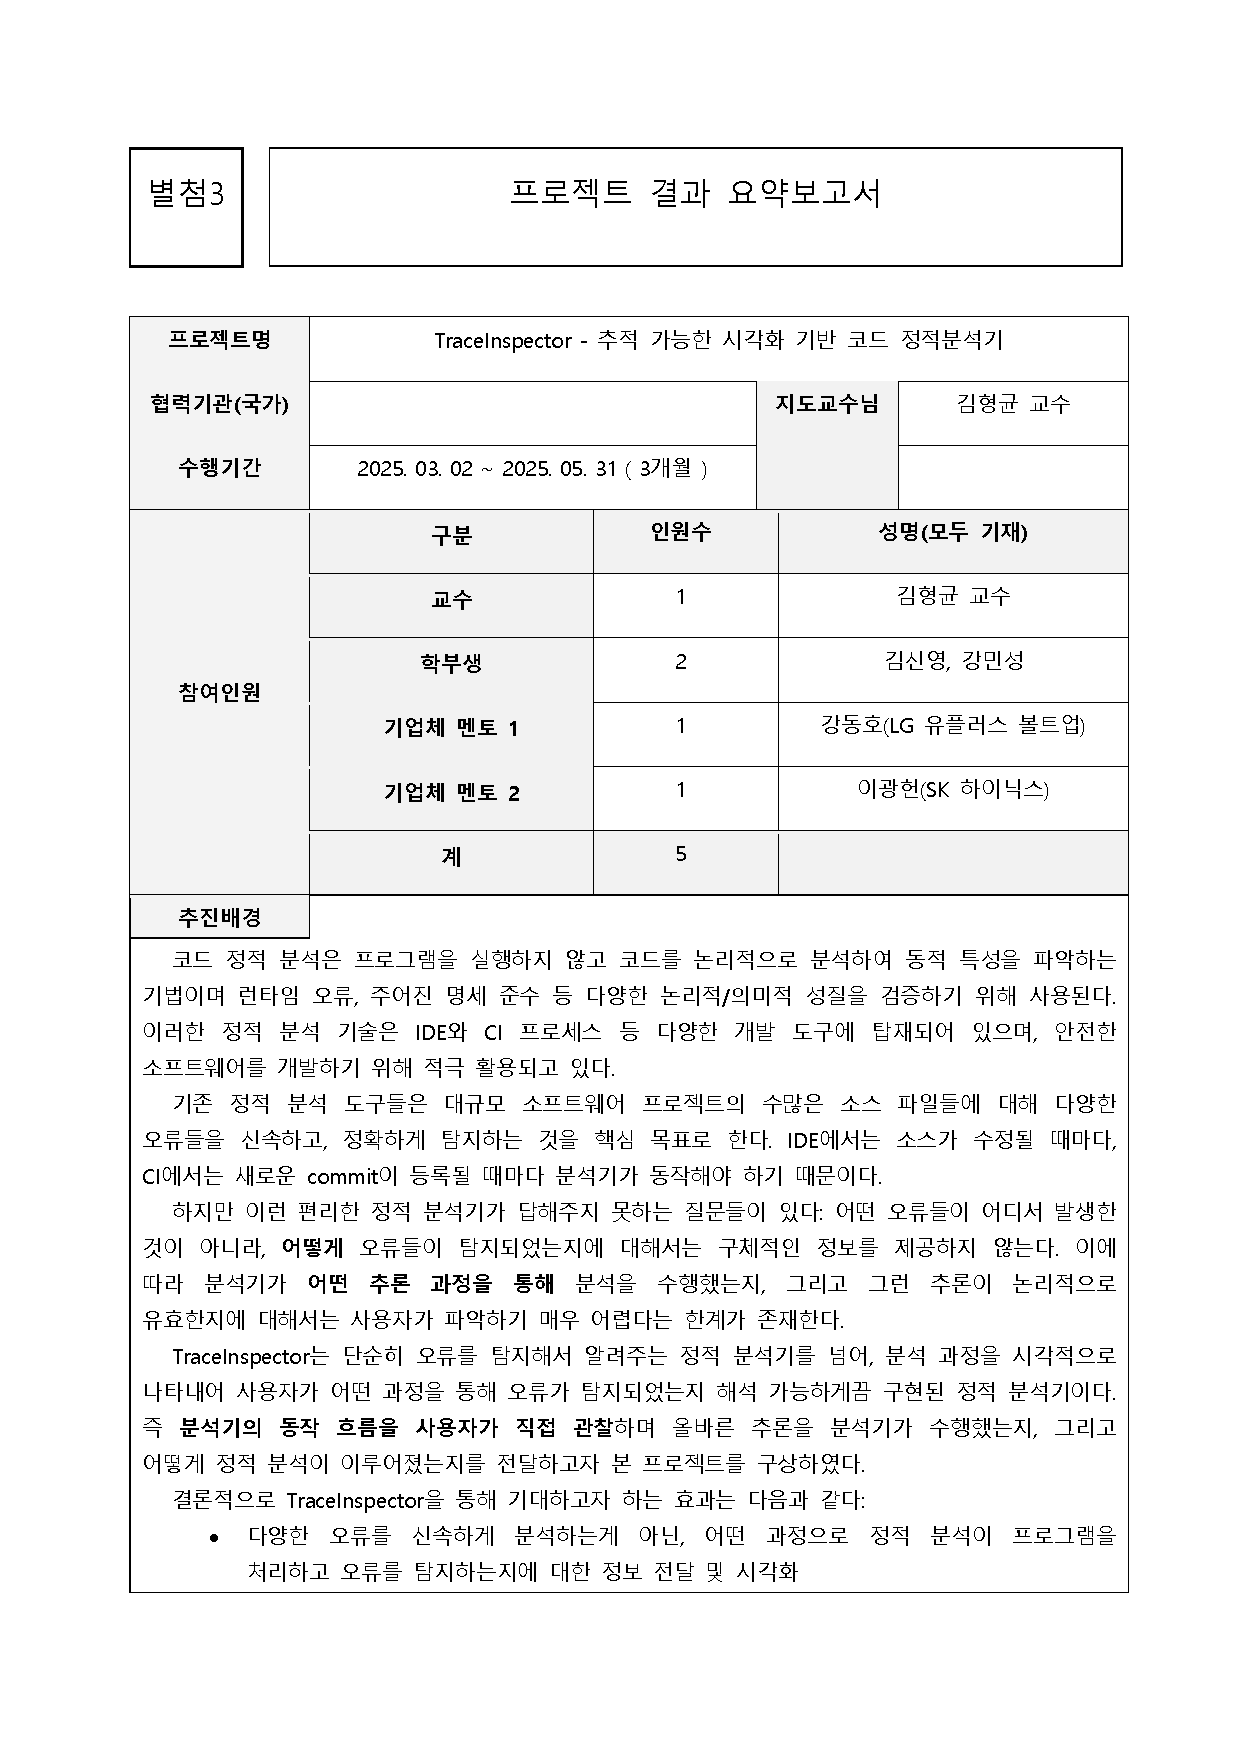
\includepdf[pages=-]{style/summary.pdf}


\begin{titlepage}
\thispagestyle{empty}

\centering

\vspace{1cm}

\Huge 제 2 장

\vspace{2.5cm}

{\fontsize{42pt}{42pt}
    중간 보고서 발표자료
    \par
}

% \vspace{1cm}
% \rule{9cm}{3.5pt}
% \vspace{1cm}

% \begin{minipage}{0.5\textwidth}
%     \raggedright
%     \Large 3.1 결과보고서 \\
%     3.2 결과보고서 발표자료 \\
% \end{minipage} \par
% \vspace{1cm}
% \rule{9cm}{3.5pt}
\end{titlepage}
\setlength{\fboxrule}{0.15pt}
\newcommand{\slidepair}[2]{
\clearpage
\thispagestyle{empty}

\begin{center}
    \fbox{
        \includegraphics[
            width=\textwidth,
            height=0.45\textheight,
            keepaspectratio
        ]{#1}
    }

    \vfill

    \fbox{
        \includegraphics[
            width=\textwidth,
            height=0.45\textheight,
            keepaspectratio
        ]{#2}
    }
\end{center}
}

\slidepair{images/mid_presentation/Slide1.png}{images/mid_presentation/Slide2.png}
\slidepair{images/mid_presentation/Slide3.png}{images/mid_presentation/Slide4.png}
\slidepair{images/mid_presentation/Slide5.png}{images/mid_presentation/Slide6.png}
\slidepair{images/mid_presentation/Slide7.png}{images/mid_presentation/Slide8.png}
\slidepair{images/mid_presentation/Slide9.png}{images/mid_presentation/Slide10.png}
\slidepair{images/mid_presentation/Slide11.png}{images/mid_presentation/Slide12.png}
\slidepair{images/mid_presentation/Slide13.png}{images/mid_presentation/Slide14.png}
\slidepair{images/mid_presentation/Slide15.png}{images/mid_presentation/Slide16.png}
\clearpage
\thispagestyle{empty}

\begin{center}
    \fbox{
        
\includegraphics[
            width=\textwidth,
            height=0.45\textheight,
            keepaspectratio
        ]{images/mid_presentation/Slide17.png}
    }

    \vfill
\end{center}
\clearpage

\input{style/final_section_title.tex}
\input{style/final_title.tex}

\setcounter{page}{1}

\renewcommand{\contentsname}{목 차}
\renewcommand{\cfttoctitlefont}{\hfill\Large\bfseries}
\renewcommand{\cftaftertoctitle}{\hfill}
\renewcommand{\cftdotsep}{1}
\setcounter{secnumdepth}{4}
\setcounter{tocdepth}{5}

\tableofcontents
\clearpage

\renewcommand{\figurename}{그림}
\renewcommand{\lstlistingname}{코드}

\newtheorem*{utheorem}{정리}
\newtheorem*{udefinition}{정의}

\onehalfspacing

\section{개요}

\subsection{프로젝트 개요}

\textsf{TraceInspector}는 요약해석(abstract interpretation)에 기반한 정적 분석기이다.
% What TraceInspector is
% Visual static analyzer
% Replayable abstract interpretation
% Educational/interpretability focus
\subsection{추진 배경 및 필요성}

올바르고 안전한 코드를 작성하는 것은 모든 프로그래머의 목표이다. 그러나 현대의 프로그래밍 환경은 고도의 추상화와 복잡한 소프트웨어 구성 요소들로 이루어져 있어, 
처음부터 완전히 안전한 코드를 작성하는 것은 사실상 불가능에 가깝다. 대신 개발자는 코드를 작성하고, 오류를 탐지하며, 디버깅을 통해 문제를 수정하는 과정을 
반복함으로써 점진적으로 프로그램의 안전성과 신뢰성을 향상시킨다.

이 과정에서 오류를 효과적으로 탐지하는 것은 매우 중요하다. 오류가 탐지되어야만 디버깅 과정이 시작될 수 있으며, 프로그램에 존재하는 문제의 원인과 위치를
 파악할 수 있기 때문이다. 따라서 소프트웨어 개발 과정에서는 단위 테스트(unit testing), 통합 테스트(integration testing), 코드 리뷰(code review), 
 정적 분석(static analysis) 등 다양한 오류 탐지 기법들이 적극적으로 활용된다.

정적 프로그램 분석(static program analysis)이란 프로그램을 직접 실행하지 않고 소스 코드를 분석하여 실제 동작 특성을 추론하는 기법들을 의미힌다.
\begin{figure}[h]
    \centering
    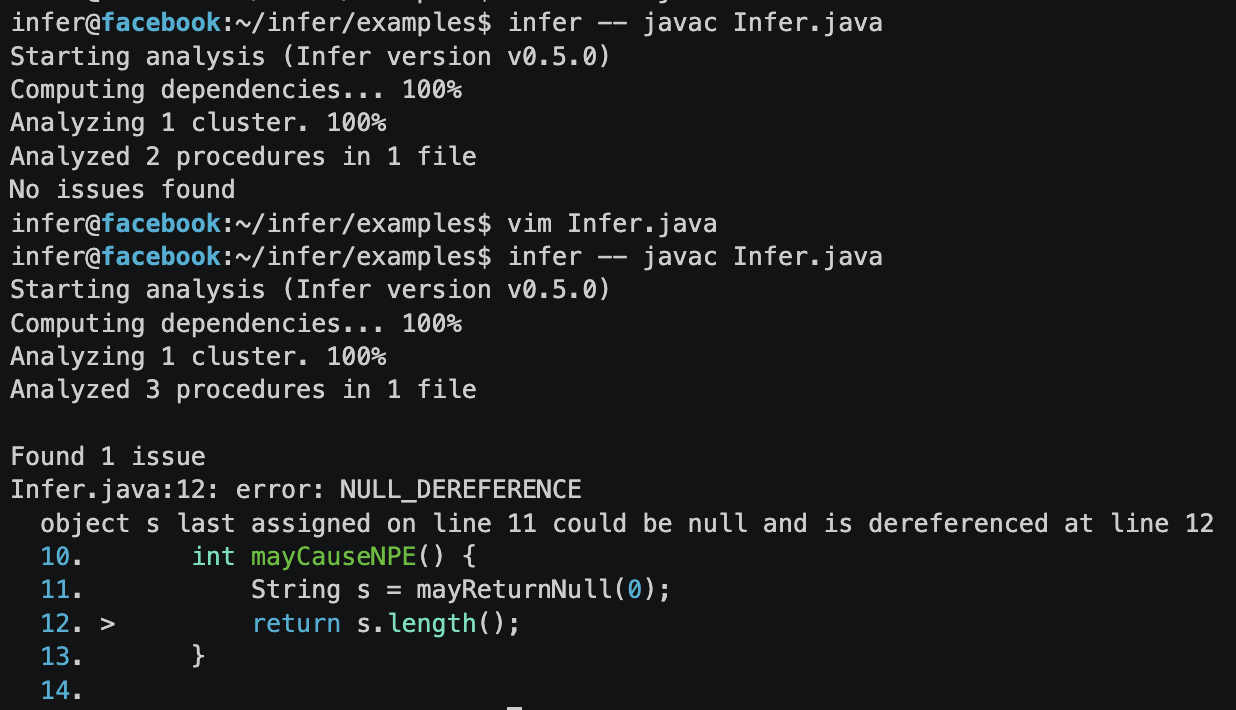
\includegraphics[width=0.7\textwidth]{images/fbinfer.png}
    \caption{Infer 분석기를 이용해 Java 코드의 \textsf{NullPointerException을} 탐지하는 모습}
\end{figure}

IDE에서 코드를 저장할 때마다 표시되는 unused variable 등의 경보, 컴파일러에서 보다 효율적인 코드 생성을 위해 수행하는 dataflow analysis, CI/CD
절차에서 커밋 후 수행되는 code linter 등 개발의 전 과정에서 프로그래머가 알게 모르게 활용되고 있다.

Facebook Infer\cite{calcagno2011}, clang static analyzer\cite{kremenek2008}
등 실제 프로그래머가 활용하여 오류를 탐지하고자 하는 목적으로 작성된 정적 분석기와, LLVM\cite{lattner2004} 등의 컴파일러 내부에서 중간 절차로 활용되는
경우와 같이 사용 환경과 분석 목표는 서로 다르지만, 공통적으로 다음과 같은 목표를 가진다:

\begin{itemize}
    \item 정확성: 의미 있는 오류 정보를 정확하게 제공해야 한다.
    \item 신속성: 분석 과정이 신속해야 하며, 지나치게 많은 시공간 자원을 소모해서는 안된다.
    \item 편리성 및 자동화: 최소한의 사용자 개입 및 추가적인 정보 없이 독자적으로 동작해야 한다.
\end{itemize}
즉 대량의 코드에 대해 빠르고 정확하게 분석하는 것을 목표로 한다. 

하지만 우리가 정적 분석기를 활용하면서, 한번쯤은 다음과 같은 질문들을 해볼 수 있다:
\begin{itemize}
    \item 정적 분석기는 어떤 과정을 통해 코드 속의 오류를 탐지할 수 있을까?
    \item 이러한 정적 분석기의 결과를 우리가 신뢰할 수 있을까?
    \item 왜 "정적"일까?
\end{itemize}

이러한 질문들은 개발자에게 익숙한 일상적 경험으로 인해 간과되기 쉽다. 
하지만 단순히 코드를 입력으로 넣었을 때 오류 정보를 알려주는 "마법의 상자"로 생각하지 않고, 그 내부의 추론 과정과 분석 원리를 이해할 수 있다면,
분석 결과를 보다 효과적으로 해석하고 활용할 수 있을 것이다.

\textsf{TraceInspector}는 위와 같은 궁금증을 해소하고자 하는 취지에서 개발되었다. 정적 프로그램 분석 기법 중 요약해석(abstract interpretation)
이론에 대해 소개하고, 단순히 어떤 오류가 존재하는지에 대한 정보를 제공하는 것을 넘어 "어떻게" 해당 이론을 통해 탐지되었는지 시각화하여 보여주고자 한다. 이를 통해 
프로그래머들에게 정적 분석 이론에 대한 이해와 친숙도를 높이고, 단순히 코드를 작성하는 행위를 넘어 논증의 대상으로 바라보는 관점을 소개하고자 한다.

알고리즘 혹은 자료구조 강의를 생각해보자. 이를테면 그래프 탐색 알고리즘을 처음 접했을 때, 알고리즘의 수학적 내용과 의사 코드만 보아서는 온전히 해당 개념을 직관적으로 이해하기 어렵다.
대신 실제 그래프 위에서 동작하는 예시를 통해 비로소 직관적인 이해가 가능해지는 경우가 많다. 특히나 알고리즘과 같이 추상화의 정도가 높은 주제의 경우 더더욱 
그럴 것이다. 마찬가지로 \textsf{TraceInspector} 역시 정적 분석 알고리즘을 시각화하여 동작 원리에 대해 와닿을 수 있는 설명을 제시하는 것이 목표이다.

\section{개발 내용 및 결과물}
\subsection{목표}

정적 분석기는 정확성과 신뢰성이 중요하다. 실제로 오류를 탐지한 경우 그 정보를 바탕으로 프로그래머는 코드를 검토하고 개발의 방향에 영향을 주는 만큼 중요한 소프트웨어이다.
따라서 점점 프로그래밍 언어와 코드베이스가 복잡해지면서 정적 코드 분석기의 구현에 대한 신뢰성과 안전성을 검증하는것 역시 못지않게 중요하다고 볼 수 있다.

Frama-C\cite{kirchner2015}, ASTR{\'E}E\cite{cousot2005}와 같은 정적 분석기들은 광범위하게 활용 가능한 실용적인 정적 분석기임과 동시에 탄탄한 이론적 바탕을 
기반으로 하여 신뢰성을 보장하고자 한다. 심지어 Verasco\cite{Jourdan15} 프로젝트는 Rocq(구 Coq)\cite{coq2024}정리 증명 언어로 정형 검증된 정적 분석기이며, 
이에 따라 분석기의 논리적 건정성이 증명된 안전한 분석기이다.

이처럼 프로그램을 "잘" 분석하는 분석기를 구현하기 위해선 신뢰할 수 있는 탄탄한 이론적 바탕이 필요함을 알 수 있게 되었다. 

\begin{figure}[h]
    \centering
    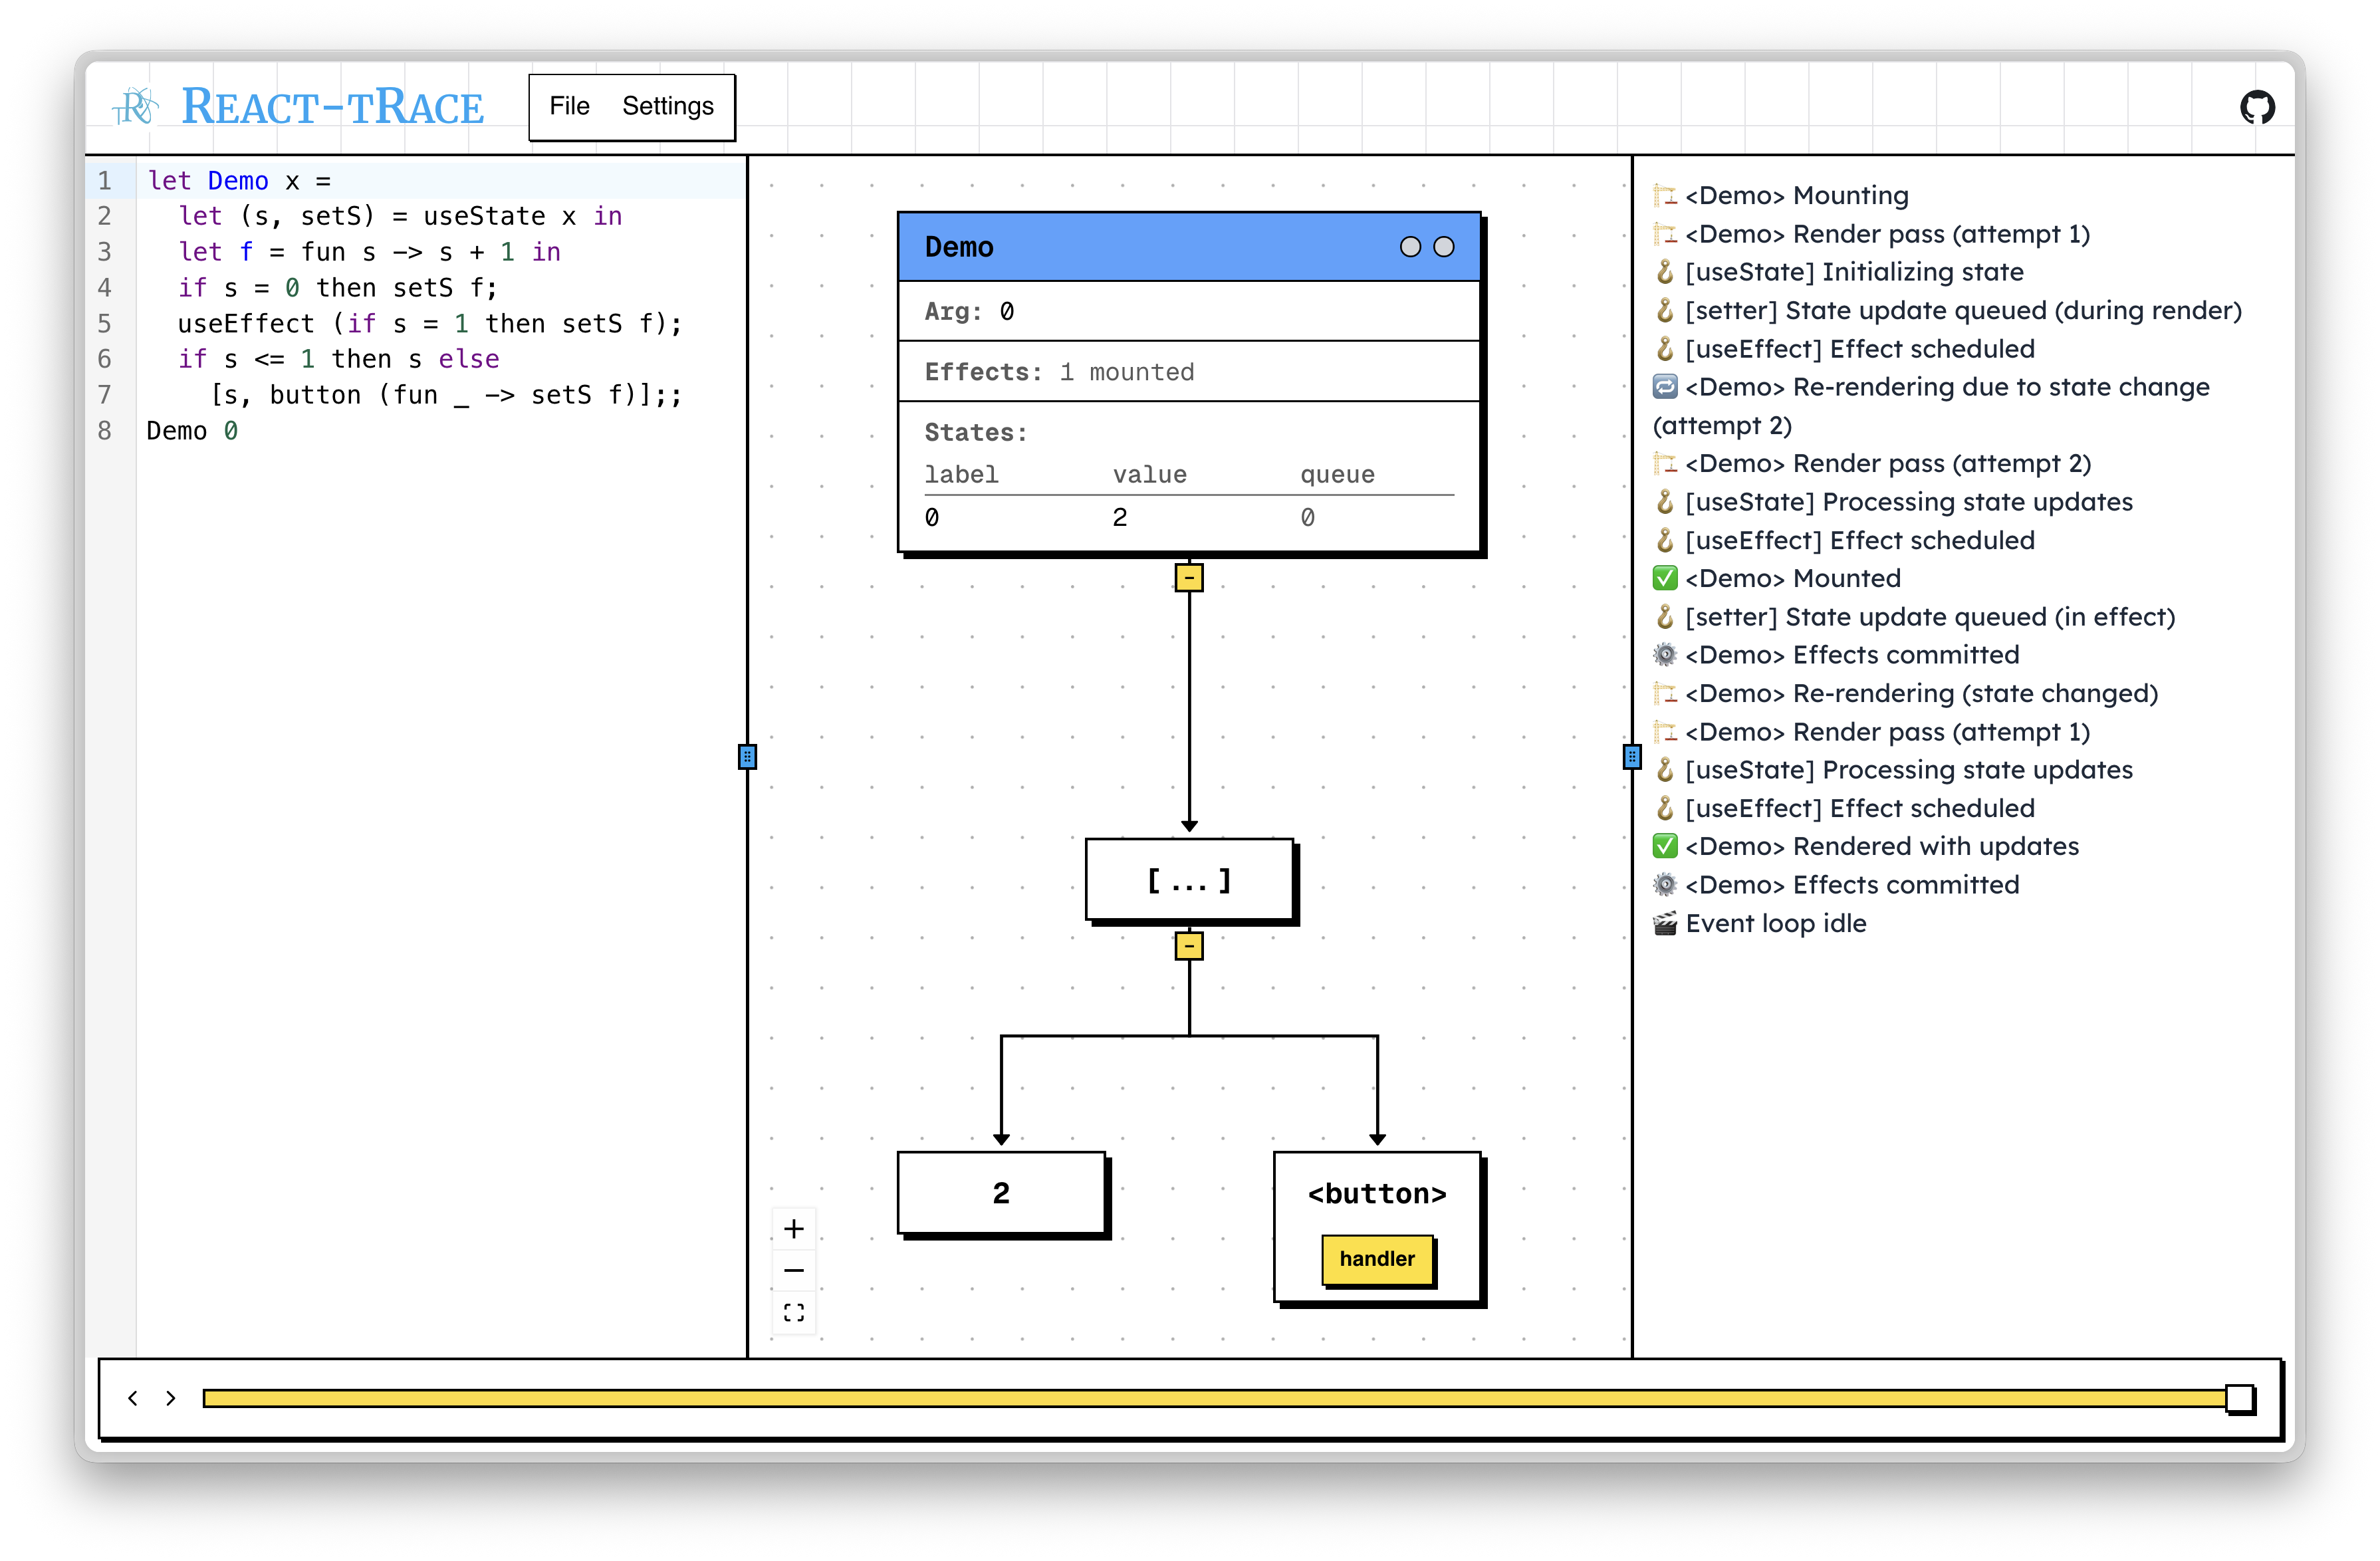
\includegraphics[width=0.8\textwidth]{images/react_trace.png}
    \caption{react-tRace의 시각화 인터페이스}
    \label{fig:react-trace}
\end{figure}

\textit{React-tRace}\cite{lee2025}는 React 웹 프레임워크의 Hook가 어떤 과정을 따라 컴포넌트를 변화시키는지 단계적인 형식 의미론을 정의한 연구이다. 
\textit{React-tRace}의 흥미로운 부분은 기존 형식 의미론 연구와는 다르게 웹 인터페이스(그림 \ref{fig:react-trace})를 통해 사용자가 직접 해당 의미론에 따라 웹페이지 컴포넌트의 상태 변화를 직접 관찰할 수 있게 해준 점이다.
따라서 단순하게 수식으로 정의한 의미론을 읽는 것을 넘어 각 변화 단계가 어떤 수식에 의해 변했는지 구체적으로 추론하고 이해할 수 있다는 점이 직관적으로 와닿고, 복잡한 알고리즘을 이해하기에 탁월한 방법임을 파악하게 되었다.

\traceinspector는 해당 연구로부터 영감을 받아 단순히 오류를 탐지해서 알려주는 정적 분석기를 넘어, 분석 과정을 시각적으로 나타내어 사용자가 어떤 과정을 통해 오류가 탐지되었는지 해석 가능하게끔 구현된 정적 분석기이다.
즉 분석기의 동작 흐름을 사용자가 직접 관찰하며 올바른 추론을 분석기가 수행했는지, 그리고 어떻게 정적 분석이 이루어졌는지를 전달하고자 본 프로젝트를 구상하였다.
다양한 오류를 신속하게 분석하는게 아닌 어떤 과정으로 정적 분석이 프로그램을 처리하고 오류를 탐지하는지에 대한 정보 전달 및 시각화를 목표로 하며, 이에 따른 프로그래밍 언어론과 정적 분석 이론에 대한 교육적 자료로 활용되기를 바란다.

앞서 설명한 목표와 같이, \textit{React-tRace}의 형식 의미론처럼 신뢰 가능하고 이론적으로 건전한 분석기를 구현하는 것을 목표로 하였다. 이에 따라 기존 정적 분석기보다는 높은 수준의 신뢰성을 추구할 수 있도록 설계하였고 요약해석 이론을 도입하여 엄밀한 명세와 정의를 바탕으로 정적 분석기를 구현하였다.

% project goals
% what you intended to demonstrate
% interpretability
% replay visualization
% educational value
% soundness-oriented analysis

\subsection{연구/개발 내용 및 결과물}
\subsubsection{연구/개발 내용}
\textsf{TraceInspector}는 요약해석 이론을 구현하여 소스 코드를 분석하는 "분석기"와 분석과 관련된 정보를 시각화하여 나타내는 "인터페이스"로 구성되어 있다.

다음은 각 요소별 설명이다.

\paragraph{\textsf{TraceInspector} 분석기} ~\\

\textsf{TraceInspector} 분석기는 Go 언어 소스 코드를 입력으로 받아, 다음의 정보를 출력하는 단일 실행 파일(executable)이다:
\begin{itemize}
    \item 제어 흐름 그래프(control-flow graph): 입력 소스 코드에 대응되는 제어 흐름 그래프
    \item 오류 정보: 입력 소스에서 발생할 수 있는 오류의 유형과 코드상 위치
    \item 분석 단계별 상태: 분석을 수행하며 단계적으로 계산된 중간 계산 결과
\end{itemize}

명령줄 인자를 통해 .go 파일을 입력받으며, 위의 정보는 모두 표준화된 JSON 형식으로 출력된다. 이에 따라 향후 \textsf{TraceInspector} 인터페이스 뿐만 아니라 
IDE와의 통합 등도 가능하다.

정적 분석은 "프로그램의 실제 실행 동작을 코드 분석을 통해 추론하는 과정"이다. 그렇다면 실제 실행 동작이 무엇인지, 코드 분석은 어떻게 할 것인지, 그리고 무엇을
추론할지에 대해서도 정의해야 한다. 각 요소들이 어떻게 정의되는지 보다 엄밀한 소개를 하고자 한다.

\subparagraph{배경: 정적 프로그램 분석과 결정가능성(decidability)} ~\\

상술했듯이 정적 프로그램 분석은 실행하지 않고 동작 특성을 추론하는 기법이다. 동작 특성의 경우 다음과 같은 예시들이 존재한다:

\begin{itemize}
    \item 0으로의 나눗셈을 수행하게끔 하는 입력이 존재하는가?
    \item 배열 인덱싱은 항상 올바른 범위 내에서 수행되는가?
    \item null 포인터를 참조하지 않는가?
    \item 로그인하지 않은 상태에서 사용자 정보에 접근할 수 있는가?
    \item 모든 입력에 대해 프로그램이 유한한 시간 내에 종료하는가?
\end{itemize}

이처럼 실행했을 때의 행동과 관련되어 있고, 참 또는 거짓으로 판별되는 명제들을 의미론적 성질(semantic property)로 칭하게 된다. "의미론적" 성질인 이유는 
단순히 프로그램의 겉모양인 구문(syntax)만 분석해서 판별할 수 없기 때문이다. 

코드 \ref{collatz}은 콜라츠 수열(Collatz sequence)의 $n$번항을 계산하는 함수이며 다음과 같은 정의를 가진다:
$$
C(n) =
\begin{cases}
    \frac{n}{2} & n \text{ 은 짝수인 경우} \\
    3n + 1 & n \text{ 은 홀수인 경우}
\end{cases}
$$

\begin{figure}[h]
  \centering % Centers the content horizontally
  \begin{minipage}{0.6\textwidth} % Limits width so centering is visible
    \begin{lstlisting}[language=python, caption={Collatz 수열을 계산하는 코드}, label={collatz}, captionpos=b]
def collatz(n):
    if n == 1:
        return 1
    if n % 2 == 0:
        return collatz(n / 2)
    else:
        return collatz(3 * n + 1)
    \end{lstlisting}
  \end{minipage}
\end{figure}

모든 양수 $n$에 대해서 위 함수가 종료할까? 1937년도에 수학자 콜라츠는 "그렇다"고 추측했지만, 아직까지도 그가 맞았다는 증명이 존재하지 않는다.
이에 따라 특정 입력값에 대해서는 실행을 통해 확인할 수 있지만, 모든 양수 입력에 대해 종료함을 보장하는 일반적인 방법은 현재까지 알려져 있지 않다.

비슷하게 튜링의 유명한 정지 문제(halting problem)\cite{turing1936}가 있다: 튜링의 정지 문제는 "임의의 프로그램이 주어졌을 때, 해당 프로그램이 유한한 시간 내에 정지할지 정확히 판별하는
프로그램은 존재할 수 없다"는 정리이다.

콜라츠 추측과 정지 문제와 같이 우리는 답을 정확히 알 수 없는 의미론적 성질이 존재함을 알게 되었다. 그렇다면 비자명한 의미론적 성질 중 자동으로 완벽하게 판별 가능한 것이 단 하나라도 존재할까? 놀랍게도
Rice 정리에 의하면 \textbf{존재하지 않는다}:

\begin{utheorem}[Rice\cite{rice1953}, 1953]
	$L$ 이 튜링 완성 언어이고, $P$가 $L$의 프로그램들에 대한 비자명한\footnote{non-trivial: 일부 프로그램에 대해서는 참이고, 일부 프로그램에 대해서는 거짓인 성질} 의미론적 성질일 때, $L$의 모든 프로그램 $p$에 대해
$$
    A(p)=
\begin{cases}
\text{참} & p \text{ 가 } P \text{ 를 만족하는 경우} \\
\text{거짓} &p \text{ 가 }  P \text{ 를 만족하지 않는 경우}
\end{cases}
$$
를 만족하는 판별 알고리즘 $A$는 존재하지 않는다.
\end{utheorem}

이를 풀어 말하자면 어떤 튜링 완성 언어로 작성된 임의의 프로그램 $p$가 성질 $P$ 를 만족하는지 완벽하게 판별 가능한 알고리즘은 존재할 수 없다는 의미이다. 
여기서 $P$를 ”프로그램이 언젠가는 종료한다” 로 한정하면 정지 문제가 된다.

논리학과 계산과학에서는 이처럼 어떤 명제에 대해 참 또는 거짓을 판별할 수 있는 알고리즘의 존재 여부를 결정가능성(decidability)\cite{moller2012} 이라고 칭한다.
이러한 관점에서 정적 프로그램 분석은 의미론적 성질을 판병하는 문제이기에 결정 불가능(undecidable)하며, 이에 따라 "모든 프로그램"에 대해 "자동으로", "완벽한" 정확성을 가지는 정적 분석기는 구현이 불가능하다.

결국 ”모든 프로그램에 대해 동작”, ”사용자의 개입 없는 알고리즘”, ”완벽한 정확성(분석 결과가 실제 오류 존재 여부와 동치)” 중 최소한 하나의 조건은 포기해야 분석기 구현이 가능해진다.

\subparagraph{배경: 프로그램 의미론} ~\\

프로그램이 실행되었을 때 동작하는 과정을 어떻게 표현할까? 단순하게 생각하면 메모리의 특정한 위치에 특정한 값을 계산한 후 저장한다고 정의할 수 있다. 형식 프로그램 의미론(formal program semantics)은
이러한 프로그램의 동작 과정에 대한 엄밀한 수학적 모형을 제시한다. 본 문서에서는 형식 의미론 중 operational semantics에 대해 소개하고자 한다. 
\textsf{TraceInspector}의 요약해석 구현이 operational semantics 위에서 정의되었기 때문이다.

Operational semantics는 프로그램 실행 과정을 프로그램 상태간의 전이로 나타내는 기법이다. 그림 \ref{fig:trace}는 어떤 시작 메모리 상태 $S$로부터 프로그램이 실행을 시작해서
$a_1, a_2, \ldots, a_n$ 중 하나의 상태로 전이되고, 이후에 후속 상태들로 계속해서 전이하는 구조로 나타낸 예시이다. 마치 오토마타에서 시작 상태에서부터 
주어진 규칙과 입력에 의해 다음 상태로 전이되는 것과 같이, 프로그램 의미론 역시 주어진 상태와 입력에서 언어의 문법적 요소별로 정해진 규칙에 따라 다음 상태로 전이되는 체계로 
나타낸 형식이다. 

요약해석 맥락에서는 이처럼 실제 프로그램 실행을 묘사하는 의미론을 "구체적 의미론(concrete semantics)"이라 칭한다. 
\textsf{TraceInspector}에서 정의한 구체적 의미론 전체는 \ref{formal_semantics}에 수록하였다.

이러한 구체적 의미론 위에서 주어진 입력과 초기 상태에 대해 실행 시 거치는 상태들의 연속을 실행 흔적(trace)라 칭한다.
$S \hookrightarrow a_1 \hookrightarrow b_1 \hookrightarrow c_1$ 흔적을 예시로 살펴보면, 시작 상태 $S$로부터 $a_1, b_1$을 거쳐 최종 상태 $c_1$에서 종료된 하나의 실행 흔적이다.

\begin{figure}[h]
    \centering
    \begin{tikzpicture}[
    >=Stealth,
    node distance=1.8cm and 1.5cm,
    every node/.style={
        circle,
        draw=cyan!20!black,
        thick,
        minimum size=10mm,
        inner sep=0pt,
        fill=gray!10
    },
    edge/.style={
        ->,
        thick
    },
    active/.style={
        fill=red!85,
        draw=cyan!20!black
    },
    pathline/.style={
        red,
        ultra thick
    }
]

% Layer 0
\node (s) at (0,0) {$S$};

% Layer 1
\node (a1) at (2,3) {$a_1$};
\node (a2) at (2,1.5) {$a_2$};
\node (a3) at (2,0) {$a_3$};
\node (a4) at (2,-1.5) {$a_4$};
\node (a5) at (2,-3) {$a_5$};

% Layer 2
\node (b1) at (4,4) {$b_1$};
\node (b2) at (4,2) {};
\node (b3) at (4,0) {};
\node (b4) at (4,-2) {};
\node (b5) at (4,-4) {};

% Layer 3
\node (c1) at (6,4) {$c_1$};
\node (c2) at (6,2) {};
\node (c3) at (6,0) {};
\node (c4) at (6,-2) {};
\node (c5) at (6,-4) {};

% Layer 4
\node (d1) at (8,2) {};
\node (d2) at (8,0) {};
\node (d3) at (8,-2) {};
\node (d4) at (8,-4) {};

% Layer 5
\node (e1) at (10,1) {};
\node (e2) at (10,-1) {};
\node (e3) at (10,-3.5) {};

% Layer 6
\node (f1) at (12,2) {};
\node (f2) at (12,0) {};
\node (f3) at (12,-2) {};
\node (f4) at (12,-4) {};

% Edges
\draw[edge] (s) -- (a1);
\draw[edge] (s) -- (a2);
\draw[edge] (s) -- (a3);
\draw[edge] (s) -- (a4);
\draw[edge] (s) -- (a5);

\draw[edge] (a1) -- (b1);
\draw[edge] (a2) -- (b2);
\draw[edge] (a3) -- (b3);
\draw[edge] (a4) -- (b4);
\draw[edge] (a5) -- (b5);

\draw[edge] (b1) -- (c1);
\draw[edge] (b2) -- (c2);
\draw[edge] (b3) -- (c3);
\draw[edge] (b4) -- (c4);
\draw[edge] (b5) -- (c5);

% \draw[edge] (c1) -- (d1);
\draw[edge] (c2) -- (d1);
\draw[edge] (c2) -- (d2);
\draw[edge] (c3) -- (d3);
\draw[edge] (c4) -- (d4);

\draw[edge] (d2) -- (e1);
\draw[edge] (d2) -- (e2);
\draw[edge] (d3) -- (e2);
\draw[edge] (d3) -- (e3);

\draw[edge] (e1) -- (f1);
\draw[edge] (e2) -- (f2);
\draw[edge] (e3) -- (f3);
\draw[edge] (e3) -- (f4);

% Highlighted propagation paths
% \draw[pathline]
% (s.center) --
% (a2.center) --
% (b2.center) --
% (c2.center) --
% (d1.center);

% \draw[pathline]
% (s.center) --
% (a2.center) --
% (b2.center) --
% (c2.center) --
% (d2.center);

% \draw[pathline]
% (s.center) --
% (a3.center) --
% (b3.center) --
% (c3.center) --
% (d3.center);

\end{tikzpicture}
    \caption{프로그램 상태 간 전이를 통해 의미를 나타내는 operational semantics}
    \label{fig:trace}
\end{figure}

오류 상태란 어떤 명제 $P$를 만족하는(혹은 만족하지 않는) 상태들의 집합이라 볼 수 있다. 그림 \ref{fig:trace_error}에선 오류 상태들을 $e_1, \cdots ,e_7$ 로 정의하였다.
이에 따라 프로그램의 초기 상태로부터 시작하여 $e_n$에 도달 가능한 경로 $S \hookrightarrow a_n \hookrightarrow \ldots \hookrightarrow e_n$ 가 존재하는 경우 오류가 발생할 수 있는 프로그램으로 정의할 수 있다.

\begin{figure}[h]
    \centering
    \input{figures/trace_error.tex}
    \caption{오류 상태 및 흔적}
    \label{fig:trace_error}
\end{figure}

\subparagraph{배경: 요약해석(abstract interpretation)} ~\\

이제 프로그램이란 메모리 상태간의 전이이고, 전이 방법은 해당 프로그래밍 언어의 형식 의미론에 의해 정해지며, 오류란 특정한 조건을 만족하는 메모리 상태이며, 
시작 상태로부터 도달 가능한 오류 상태가 존재하는 경우 오류가 존재하는 프로그램이라는 것을 정의하였다.

요약해석 이론은 논리적으로 건전한(sound) 분석을 목표로 한다. 신뢰할 수 있는 분석기를 만든다는 것은 다양한 해석이 가능하겠지만 그중 "오류가 없다고 분석된다면 실제로 실행 가능한 모든 경로에 대 오류 흔적은 존재하지 않는다" 고 정의할 수 있으며,
이 문장이 논리적 건정성을 한 문장으로 표현한 것이다.

입력 프로그램 $p$에 대해, $analysis(p)$는 $p$에 대한 분석을 수행하며, 그 결과로 "오류가 존재한다"와 "오류가 존재하지 않는다"를 반환한다.
$error(p)$는 $p$를 실행했을 때 오류가 발생 가능한지 판별하는 오라클(oracle) 함수이다. 여기서 오라클이랑 실제로 구현 불가능하지만 완벽하게 사실을 판별할 수 있는 가상의 함수이다.
$analysis(p)$ 가 논리적으로 건전하기 위해선
\begin{equation}
    analysis(p) = \text{"오류가 존재하지 않는다"} \Rightarrow error(p) = \text{"오류가 존재하지 않는다"}
\end{equation}
를 만족해야 한다.\footnote{더 일반적이고 엄밀한 정의는 임의의 의미론적 명제 $P$에 대해 $analysis(p, P) = true \Rightarrow P \ p$ 이다.} 이 조건은 오류가 존재하지 않는 분석 결과에 대해서는 보증을 하지만, 반면 분석 결과가 "오류가 존재한다"인 경우 어떠한 보증도 하지 않게 된다.
실제로 실행했을 때 오류가 발생할수도 있지만 그렇지 않고 존재하지 않는 오류에 대한 허위 경보(false positie)를 낼 수도 있다는 의미이다. 앞서 설명한 Rice 정리의 직접적인 영향 때문이다.

\begin{figure}[h]
    \centering
    \begin{tikzpicture}[
    >=Stealth,
    node distance=1.8cm and 1.5cm,
    every node/.style={
        circle,
        draw=cyan!20!black,
        thick,
        minimum size=10mm,
        inner sep=0pt,
        fill=gray!10
    },
    edge/.style={
        ->,
        thick
    },
    active/.style={
        fill=red!85,
        draw=cyan!20!black
    },
    pathline/.style={
        red,
        ultra thick
    }
]

% Layer 0
\node (s) at (0,0) {$S$};

% Layer 1
\node (a1) at (2,3) {};
\node (a2) at (2,1.5) {};
\node (a3) at (2,0) {};
\node (a4) at (2,-1.5) {};
\node (a5) at (2,-3) {};

% Layer 2
\node (b1) at (4,4) {};
\node (b2) at (4,2) {};
\node (b3) at (4,0) {};
\node (b4) at (4,-2) {};
\node (b5) at (4,-4) {};

% Layer 3
\node (c1) at (6,4) {};
\node (c2) at (6,2) {};
\node (c3) at (6,0) {};
\node (c4) at (6,-2) {};
\node (c5) at (6,-4) {};

% Layer 4
\node[active] (d1) at (8,2) {$e_1$};
\node[active] (d2) at (8,0) {$e_2$};
\node[active] (d3) at (8,-2) {$e_3$};
\node (d4) at (8,-4) {};

% Layer 5
\node[active] (e1) at (10,1) {$e_4$};
\node[active] (e2) at (10,-1) {$e_5$};
\node (e3) at (10,-3.5) {};

% Layer 6
\node[active] (f1) at (12,2) {$e_6$};
\node[active] (f2) at (12,0) {$e_7$};
\node (f3) at (12,-2) {};
\node (f4) at (12,-4) {};

% Edges
\draw[edge] (s) -- (a1);
\draw[edge] (s) -- (a2);
\draw[edge] (s) -- (a3);
\draw[edge] (s) -- (a4);
\draw[edge] (s) -- (a5);

\draw[edge] (a1) -- (b1);
\draw[edge] (a2) -- (b2);
\draw[edge] (a3) -- (b3);
\draw[edge] (a4) -- (b4);
\draw[edge] (a5) -- (b5);

\draw[edge] (b1) -- (c1);
\draw[edge] (b2) -- (c2);
\draw[edge] (b3) -- (c3);
\draw[edge] (b4) -- (c4);
\draw[edge] (b5) -- (c5);

% \draw[edge] (c1) -- (d1);
\draw[edge] (c2) -- (d1);
\draw[edge] (c2) -- (d2);
\draw[edge] (c3) -- (d3);
\draw[edge] (c4) -- (d4);

\draw[edge] (d2) -- (e1);
\draw[edge] (d2) -- (e2);
\draw[edge] (d3) -- (e2);
\draw[edge] (d3) -- (e3);

\draw[edge] (e1) -- (f1);
\draw[edge] (e2) -- (f2);
\draw[edge] (e3) -- (f3);
\draw[edge] (e3) -- (f4);

% Highlighted propagation paths
\draw[pathline]
(s) --
(a2.center) --
(b2.center) --
(c2.center) --
(d1);

\draw[pathline]
(s) --
(a2.center) --
(b2.center) --
(c2.center) --
(d2);

\draw[pathline]
(s) --
(a3.center) --
(b3.center) --
(c3.center) --
(d3);

\node[
    rectangle,
    draw=green,
    dashed,
    fill=none,
    thick,
    inner sep=4mm,
    fit=(a1)(a2)(a3)(a4)(a5)
] {};

\node[
    rectangle,
    draw=green,
    dashed,
    fill=none,
    thick,
    inner sep=4mm,
    fit=(b1)(b2)(b3)
] {};

\node[
    rectangle,
    draw=green,
    dashed,
    fill=none,
    thick,
    inner sep=4mm,
    fit=(b4)(b5)
] {};

\node[
    rectangle,
    draw=green,
    dashed,
    fill=none,
    thick,
    inner sep=4mm,
    fit=(c1)(c2)(c3)(c4)
] {};

\node[
    rectangle,
    draw=green,
    dashed,
    fill=none,
    thick,
    inner sep=0pt,
    fit=(c5)(d4)(e3)(f4)
] {};

\node[
    rectangle,
    draw=red,
    dashed,
    fill=none,
    thick,
    inner sep=4mm,
    fit=(d1)(d2)(d3)(e1)(e2)(f1)(f2)
] {};

\end{tikzpicture}
    \caption{오류 상태의 요약}
    \label{fig:trace_error_abstraction}
\end{figure}

요약해석 이론은 실제 프로그램 상태에 대한 "보수적인" 근사치를 논리적으로 건전하게 계산하는 방법이다. 
앞서 활용한 프로그램 흔적 예시를 요약해석의 관점에서 생각해보자면, 그림 \ref{fig:trace_error_abstraction}와 같이 모든 상태들에 대한 구체적인 전이를 계산하지 않고, 초록색 상자처럼 여러개의 구체적인 상태들을 요약해서 나타낼 수 있는 "요약 상태"로 압축하여 나타내는 것이다.
오류 상태들에 대해서도 마찬가지로 구체적인 오류 상태들을 포함한 근사치(빨간색 상자)로 오류 상태를 정의하게 된다. 보수적인 근사이기 때문에 요약 오류 상태에서는 실제로는 오류 상태가 아니지만 포함된 일반 상태도 존재하게 된다. 하지만 실제 오류 상태들은 빠짐없이 요약 상태에서도 오류로 표현되어야 한다.

\begin{figure}[h]
    \centering

    \begin{subfigure}[t]{0.48\textwidth}
    \begin{lstlisting}[language=Python, mathescape]
    x = input()[x : n]
    if x < 0:
        y = -x [x : n, y : -n]
    elif x > 0:
        y = x  [x : n, y : n]
    else:
        y = 0  [x : n, y : n]
    \end{lstlisting}
    \caption{구체적 정수값}
    \end{subfigure}
    \hfill
    \begin{subfigure}[t]{0.48\textwidth}
    \begin{lstlisting}[language=Python, mathescape]
    x = input() [x : $\top$]
    if x < 0:
        y = -x  [x : -, y : +]
    elif x > 0:
        y = x   [x : +, y : +]
    else:
        y = 0   [x : 0, y : 0]
    \end{lstlisting}
    \caption{부호 도메인으로 요약}
    \end{subfigure}

    \caption{정수값과 부호 도메인}
    \label{fig:int_sign_abstraction}
\end{figure}

그림 \ref{fig:int_sign_abstraction}는 간단한 정수값을 계산하는 프로그램에 대해 구체적인 값들을 계산하는 경우와 각 변수의 부호만을 요약해서 계산하는 경우를 나타내었다.
구체적인 값의 경우 x가 임의의 입력 $n \in \mathbb{Z}$을 받은 이후, 코드에 따라 변수 값을 직접 계산하게 된다. 반면 부호로 요약한 경우 잠재적으로 가능한 입력은 모든 정수이기에,
$-, 0, +$ 중 어떤 값도 가능한 $\top$ 기호를 통해 나타나게 되고, 이후 조건에 따라 양수, 음수, 0으로 나눠서 표현하게 된다. 부호 정보만을 가지고 있기에 실제로 정수의 값을 알 순 없지만,
실제 값을 알지 못하더라도 각 분기에 들어갔을 때 가질 수 있는 값들에 대한 성질을 추론할 수 있게 된다.

조금 더 엄밀하게 생각해보면 각 코드의 지점마다 변수가 가질 수 있는 값들은 어떤 조건을 만족하는 집합으로 나타낼 수 있다. \verb|x = input()| 의 경우 정수집합 $\mathbb{Z}$ 가 가능하며, 양수의 경우
양수들의 집합 $\mathbb{Z}_{+} := \{n \ | \ n > 0\}$, 음수는 $\mathbb{Z}_{-} := \{n \ | \ n < 0\}$, 그리고 한원소 집합 $\{0\}$ 로 표현된다. 따라서 정수값들을 다루는 의미에서 프로그램 상태는
정수집합 $\mathbb{Z}$의 멱집합 $\mathcal{P}(\mathbb{Z})$가 된다.

부호들의 경우 보다 단순하다. "모든 부호"를 나타내는 $\top$와, $+, 0, -$ 로 구성되어 있다. 추가로 위 코드에서는 쓰이지 않았지만, "모든 부호"의 쌍대에 해당하는 "유효하지 않은 값들의 부호"를 나타내는 $\bot$도 추가된다.
즉 부호로 요약해서 계산하는 의미론에서는 프로그램 상태가 부호 요약도메인 $\mathrm{sign} := \{\top, +, 0, -, \bot\}$ 의 원소들로 표현된다.

\begin{figure}[h]
    \centering
    \begin{tikzpicture}[
    node distance=1cm,
    lattice/.style={},
    map/.style={->,blue,thick},
]

%----------------------------------
% Concrete lattice
%----------------------------------

\node[lattice] (cTop) {$\{-1,0,1\}$};

\node[lattice,below left=of cTop] (cNeg) {$\{-1\}$};
\node[lattice,below=of cTop] (cZero) {$\{0\}$};
\node[lattice,below right=of cTop] (cPos) {$\{1\}$};

\node[lattice,below=of cZero] (cBot) {$\emptyset$};

\draw (cTop) -- (cNeg);
\draw (cTop) -- (cZero);
\draw (cTop) -- (cPos);

\draw (cNeg) -- (cBot);
\draw (cZero) -- (cBot);
\draw (cPos) -- (cBot);

%----------------------------------
% Abstract lattice
%----------------------------------

\begin{scope}[xshift=8cm]

\node[lattice] (aTop) {$\top$};

\node[lattice,below left=of aTop] (aNeg) {$-$};
\node[lattice,below=of aTop] (aZero) {$0$};
\node[lattice,below right=of aTop] (aPos) {$+$};

\node[lattice,below=of aZero] (aBot) {$\bot$};

\draw (aTop) -- (aNeg);
\draw (aTop) -- (aZero);
\draw (aTop) -- (aPos);

\draw (aNeg) -- (aBot);
\draw (aZero) -- (aBot);
\draw (aPos) -- (aBot);

\end{scope}

%----------------------------------
% Abstraction arrows α
%----------------------------------

\draw[map]
    (cNeg.east)
    to[bend left=15]
    node[midway,above] {$\alpha$}
    (aNeg.west);

\draw[map]
    (cZero.east)
    -- (aZero.west);

\draw[map]
    (cPos.east)
    -- (aPos.west);

\draw[map]
    (cTop.east)
    to[bend left=10]
    (aTop.west);

\draw[map]
    (cBot.east)
    to[bend right=10]
    (aBot.west);

\end{tikzpicture}
    \caption{정수 집합과 부호로의 대응}
    \label{fig:int_sign_galois}
\end{figure}

따라서 부호를 계산하는 것이란 주어진 코드 지점에서 구체적인 정수값들의 집합 $s \subset \mathbb{Z}$ 에서 $\mathrm{sign}$으로 대응시키는 함수 $\alpha : \mathcal{P}(\mathbb{Z}) \rightarrow \mathrm{sign}$ 으로 볼 수 있다.
\verb|x = input()| 를 수행한 이후 $x$가 가능한 값들의 집합은 $\mathbb{Z}$이고 이에 따른 $\alpha(\mathbb{Z}) = \top$ 가 되고, 마찬가지로 $x$ 가 양수인 집합은 $\mathbb{Z}_{+}, \alpha (\mathbb{Z}_{+}) = +$ 가 된다.

\verb|x := 4|와 같은 코드가 실행된 이후 가능한 상태의 집합은 한원소 집합 $\{4\}$이다. $\alpha(\{4\}) = +$가 되는데, 이는 $\alpha(\mathbb{Z}_{+})$와 동일한 결과를 가지게 된다. 
양수들의 집합보다 구체적인 정보를 가지고 있었지만 부호로 요약되며 해당 정보를 잃게 되는 것이다. 그림 \ref{fig:int_sign_abstraction}는 정수 집합을 부호 요약도메인으로 대응시키는 예시를 보여준다.

구체적인 값들의 집합에서 요약도메인의 원소로 대응시키는 $\alpha$ 함수가 있듯이, 역으로 요약도메인의 원소에서 구체적인 값들의 집합으로 대응시키는 $\gamma: \mathrm{sign} \rightarrow \mathcal{P}(\mathbb{Z})$를 정의할 수 있다. $\gamma(\top) = \mathbb{Z}, \gamma(+) = \mathbb{Z}_{+}, \ldots$ 로 간단하게 정의된다.

두 함수 $\alpha, \gamma$에 대해서 다음과 같은 성질에 대해 생각해볼 수 있다:

\begin{itemize}
    \item 임의의 정수집합 $s \subseteq \mathbb{Z}$에 대해, $\gamma(\alpha(s))$의 결과
    \item 임의의 부호도메인의 원소 $e \in \mathrm{sign}$에 대해, $\alpha(\gamma(e))$의 결과
\end{itemize}

첫번째 경우는 $\alpha(s)$를 수행하며 구체적인 정보가 소실된다. 이예 따라서 $\{4\} \subset \mathbb{Z}_{+}$와 같이 보다 구체적인 집합을 넣더라도 같은 도메인 값 $\alpha(s)$으로 요약된다. 
$\gamma(e)$는 해당 부호를 만족하는 원소들을 전부 포함시키기에, 모든 $s \subseteq \mathbb{Z}$ 에 대해 $s \subseteq \gamma(\alpha(s))$임을 알 수 있다.\cite{cousot1977}

$\gamma(e)$의 결과는
\begin{itemize}
    \item $\gamma(\top) = \mathbb{Z}$
    \item $\gamma(\bot) = \emptyset$
    \item $\gamma(+) = \mathbb{Z}_{+}$
    \item $\gamma(0_{\mathrm{sign}}) = \{0\}$
    \item $\gamma(-) = \mathbb{Z}_{-}$
\end{itemize}
로 열거할 수 있다. 따라서 모든 $e \in \mathrm{sign}$에 대해 $e = \alpha(\gamma(e))$임을 알 수 있다.

$\alpha, \gamma$ 두 함수에 대한 이 성질들은 "보수적인" 요약이 무엇인지를 정확하게 나타내는 역할을 한다. 
구체적인 값들의 집합을 요약하여 표현한 결과는 항상 원래 값을 포함하여야 함을 정의한 것이고, 이 조건을 통해 요약 상태에서 추론을 하더라도 구체적인 상태를 빠짐없이 반영할 수 있음을 보장하게 된다.

지금까지 설명은 정수들의 집합 $\mathcal{P}(\mathbb{Z})$에 대한 순서관계 $\subseteq$가 정의된 상태에서 진행되었는데 마찬가지로 요약도메인 $\mathrm{sign}$에 대해서도 순서관계 $\sqsubseteq$를 정의할 수 있다:
$\bot$는 어떠한 값도 나타내지 않기에 $\forall e. \bot \sqsubseteq e$가 되며, 마찬가지로 $\top$는 모든 정수값을 나타내기에 $\forall e. e \sqsubseteq \top$가 성립된다. $+, 0, -$는 구체적인 상태로도 서로소 집합이기에 포함관계로도 순서 정의가 불가능하다.
이는 "부분 순서 관계(partially ordered)"로 정의가 되며, 모든 원소보다 순서 관계상 큰 $\top$ 원소와 작은 원소 $\bot$가 존재하기에 "완전 부분 순서 관계(complete partial order)"의 성질을 가지게 된다.

따라서 위에서 정의한 $\alpha, \gamma$의 두 성질은 순서 관계가 정의된 두 집합 $(\mathcal{P}(\mathbb{Z}), \subseteq)$와 $(\mathrm{sign}, \sqsubseteq)$ 사이의 "갈루아 연결(galois connection)"을 나타낸다:
\begin{udefinition}[갈루아 연결(Galois Connection)]
	프로그램의 구체적 상태들의 집합 $C$와 그 위에서의 순서 관계 $\subseteq$ 가 주어지고 요약상태 집합 $A$와 그 위에서의 순서 관계 $\sqsubseteq$가 주어졌을 때,
    두 함수 $\gamma : A \rightarrow C$와 $\alpha : C \rightarrow A$ 에 대해
    $$
    \forall c \in C. \ \forall a \in A. \ \alpha(c) \sqsubseteq a \iff c \subseteq \gamma(a)
    $$
    를 만족하면 두 집합과 순서관계 사이에 갈루아 연결을 형성한다고 정의하며, 
    $$
    (C, \subseteq) \underset{\gamma}{\overset{\alpha}{\leftrightarrows}} (A, \sqsubseteq)
    $$
    로 나타낸다.\cite{cousot2021}\cite{rival2020}
\end{udefinition}

이는 단순히 "정수와 부호"와 같이 특정한 값들과 요약 상태뿐만 아니라 일반적으로 적용할 수 있는 성질이며, 따라서 요약해석에 기반한 정적분석을 구현할 때 논리적으로 건전함을 보이기 위해선 프로그램의 구체적 상태와
요약 상태간의 갈루아 연결이 형성됨을 증명해야 한다.

\begin{figure}[h]
    \centering
    \resizebox{0.9\linewidth}{!}{
        \begin{tikzpicture}[
    >=Latex,
    domnode/.style={ellipse,draw,minimum width=2.5cm,minimum height=5cm},
    map/.style={->,thick},
]

% =====================================================
% Property 1 : c ⊆ γ(α(c))
% =====================================================

\node at (0,3.3) {\Large C};
\node at (6,3.3) {\Large A};

\node[domnode] (C1) at (0,0) {};
\node[domnode] (A1) at (6,0) {};

\node (c) at (0,-1.0) {$c$};
\node (gac) at (0,1.0) {$\gamma(\alpha(c))$};

\node (ac) at (A1.center) {$\alpha(c)$};

\draw[map,blue]
    (ac.west)
    to[bend right=15]
    node[above] {$\gamma$}
    (gac.east);

\draw[map,red]
    (c.east)
    to[bend right=15]
    node[below] {$\alpha$}
    (ac.west);

\draw[dashed]
    (c) 
    -- node[right] {$\subseteq$}
    (gac);

\node[align=center] at (3,-3.5)
{
\Large $c \subseteq \gamma(\alpha(c))$\\[0.2em]
보수적 과다추정
};

% =====================================================
% Property 2 : α(γ(a)) = a
% =====================================================

\node at (11,3.3) {\Large C};
\node at (17,3.3) {\Large A};

\node[domnode] (C2) at (11,0) {};
\node[domnode] (A2) at (17,0) {};

\node (ga) at (C2.center) {$\gamma(a)$};

\node (a) at (17,1.0) {$a$};
\node (aga) at (17,-1.0) {$\alpha(\gamma(a))$};

\draw[map,blue]
    (a.west)
    to[bend right=15]
    node[above] {$\gamma$}
    (ga.east);

\draw[map,red]
    (ga.east)
    to[bend right=15]
    node[below] {$\alpha$}
    (aga.west);

\draw[dashed]
    (a) 
    -- node[right] {$=$}
    (aga);

\node[align=center] at (14,-3.5)
{
\Large $\alpha(\gamma(a)) = a$\\[0.2em]
요약상태의 복원
};

\end{tikzpicture}
    }
    \caption{갈루아 연결과 $\alpha, \gamma$의 성질}
    \label{fig:galois_property}
\end{figure}

\traceinspector는 \verb|algebra/extended_integers.go|에 $\pm \infty$를 추가한 확장된 정수체계 $\mathbb{Z}_{\infty}$를 구현하였다.
대소관계 비교 및 산술연산이 구현되어 있으며, 이를 기반으로 \verb|domain/interval.go|에 확장된 정수체계 기반 구간도메인이 구현되어 있다.

\subparagraph{\textsf{Imp} 중간 표현 언어} ~\\

\traceinspector 의 첫 단계는 입력으로 Go 소스 파일을 받아 Go 표준 라이브러리의 \textsf{go/parser} 패키지를 이용해 추상 구문 트리(abstract syntax tree, AST)
로 파싱하는 것이다. 이후 \imp \cite{pierce2002} 라는 간단한 명령형 프로그래밍 언어 겸 중간 표현 형식으로 번역한 후 \imp AST위에서 분석 단계를 수행한다.

\imp는 다음과 같은 기능을 가진 명령형 언어이다:
\begin{itemize}
    \item \textsf{int, bool, string} 및 다차원 동적 배열 \textsf{[]T}
    \item 산술/논리 연산 및 입출력
    \item \textsf{if, while, continue, break} 제어 흐름
    \item 함수 선언 및 반환
\end{itemize}
이처럼 구조적으로 간단하지만 충분히 복잡한 수준의 프로그램을 표현할 수 있는 구조이다. 

Go AST 에 대해 직접적으로 분석을 수행하지 않는 이유는 크게 두가지가 있는데, 첫번째는 추상 구문 트리의 특성상 프로그램의 제어 흐름을 제외한 구문적 요소들이 트리에 많이 포함되어 있기 때문이다.
그림 \ref{fig:go_imp_ast}는 b라는 변수에 원소가 100인 정수형 동적 배열을 선언하는 명령 \verb|b := []int{100}|를 Go AST로 파싱한 결과와, 이를 \imp AST로 번역한 결과를 나타낸다.
Go AST의 경우 리터럴에 대해서도 종류와 값을 분리하여 표기하고, 배열 리터럴 역시 타입을 구별하여 표기하는 등 범용적이지만 복잡한 형태로 구성되어 있다.

반면 \imp 의 경우 리터럴의 타입별 정의와 배열 리터럴 등 문법적 요소를 최대한 배제한 형태로 구현하였고, 리터럴 값을 문자열로 표현한 것이 아니라 타입에 맞는 값을 직접 담게 된다. 이러한 설계는 
향후 제어 흐름 그래프 생성 등 프로그램의 형태가 아닌 동작 특성을 파악하고자 하는 경우에 훨씬 간결하고 수월하게 구현을 가능케 해준다.

\begin{figure}[t]
    \centering

    \begin{subfigure}[t]{0.48\textwidth}
        \centering
        \begin{tikzpicture}[
    level distance=1.3cm,
    sibling distance=2.5cm,
]
\node {AssignStmt}
    child { 
        node {Ident}
        child { node {"b"} } 
    }
    child {
        node {CompositeLit}
        child {
            node {ArrayType}
            child {
                node {Ident}
                child { node {"int"} }
            } 
        }
        child { 
            node {BasicLit}
            child {
                node {Kind}
                child { node {"INT"} }
            } 
            child {
                node {Value}
                child {node {"100"} }
            }
        }
    };
\end{tikzpicture}
        \caption{Go AST}
    \end{subfigure}
    \hfill
    \begin{subfigure}[t]{0.48\textwidth}
        \centering
        \begin{tikzpicture}[
    level distance=1.3cm,
    sibling distance=2.5cm,
]
\node {AssignStmt}
    child { 
        node {VarExpr}
        child { node {"b"} } 
    }
    child {
        node {ArrayLitExpr}
        child {
            node {IntLitExpr}
            child {node {100} } 
        }
    };
\end{tikzpicture}
        \caption{\imp AST}
    \end{subfigure}

    \caption{Go AST와 \imp AST 비교}
    \label{fig:go_imp_ast}
\end{figure}

두번째 이유는 특정 언어의 문법적 형태와는 독립적인 분석 기능을 구현하고자 했기 때문이다. Go 언어의 요소에 대한 요약의미론을 직접 정의할 경우 오직 Go 언어에 대해서만 분석 가능하지만,
\imp 라는 전형적인 언어를 대상으로 분석기를 구현하고자 할 경우, 향후 Go 외의 타 언어를 \imp 로 번역하는 번역기만 구현할 경우 이후 분석기 로직을 온전히 활용할 수 있다.

이처럼 입력 소스를 파싱하고 처리하는 프론트엔드와, 분석을 담당하는 미들엔드를 분리하여 각각 다른 표현상에서 동작하게끔 설계하는 방식은 현대 컴파일러에서 자주 활용되는 매우 전형적인 설계 방식이다.
\traceinspector 역시 이러한 설계 패턴을 도입하고, 구현의 편의성을 위해 \imp로의 번역 과정을 최우선적으로 수행한다.

\begin{figure}[t]
    \centering
    \[
\begin{array}{rcl}
e &::=& \mathbb{X}
      \mid \mathbb{N}
      \mid \mathbb{B}
      \mid \mathbb{S}
      \mid \{e_1,\ldots,e_n\}
\\
  &\mid& e + e
      \mid e - e
      \mid e * e
      \mid e / e
      \mid e \bmod e
\\
  &\mid& e = e
      \mid e \neq e
      \mid e < e
      \mid e \le e
      \mid e > e
      \mid e \ge e
\\
  &\mid& e \land e
      \mid e \lor e
\\
  &\mid& -e
      \mid \neg e
\\
  &\mid& (e)
      \mid e[e]
\\
  &\mid& f(e_1,\ldots,e_n)
\\
  &\mid& \mathrm{len}(e)
\\
  &\mid& \mathrm{make\_array}(e,e)
\\[1em]

s &::=& \mathbf{skip}
\\
  &\mid& x := e
\\
  &\mid& e[e] := e
\\
  &\mid& \mathbf{if}\ e\ \mathbf{then}\ \{s^*\}
      \ \mathbf{else}\ \{s^*\}
\\
  &\mid& \mathbf{while}\ e\ \mathbf{do}\ \{s^*\}
\\
  &\mid& \mathbf{break}
      \mid \mathbf{continue}
\\
  &\mid& e{++}
      \mid e{--}
\\
  &\mid& f(e_1,\ldots,e_n)
\\
  &\mid& \mathbf{print}(e_1,\ldots,e_n)
\\
  &\mid& \mathbf{scanf}(s,e_1,\ldots,e_n)
\\
  &\mid& \mathbf{return}\ e
\\[1em]

\tau &::=& \mathbf{int}
        \mid \mathbf{bool}
        \mid \mathbf{string}
\\
     &\mid& \mathbf{array}\langle\tau\rangle
\end{array}
\]

    \caption{\imp의 명령문(statement), 식(expression)들의 문법}
    \label{fig:imp_syntax}
    
\end{figure}

\imp의 문법적 정의는 그림 \ref{fig:imp_syntax}과 같으며, \imp 의 bigstep operational semantics 일부는 부록 \ref{imp_semantics}에 수록하였다.

\subparagraph{요약 도메인} ~\\

\traceinspector는 정수값을 구간 요약도메인으로, bool값을 bool 요약도메인으로, 그리고 배열을 배열 축약 요약도메인으로 요약하여 실행한다.

구간 요약도메인 $\mathbb{I}$란 가능한 정수들의 집합을 $\interval{l}{h}$ 의 닫힌 구간으로 나타낸 요약 도메인이다. 

구간 요약도메인에 대한 $\alpha, \gamma$ 정의는 다음과 같다:

\begin{itemize}
    \item $\alpha(\mathbb{Z}) = [-\infty, \infty] = \top$
    \item $\alpha(\emptyset) = \bot$
    \item $\alpha(\{x_0, x_1, \cdots, x_n\}) = [\mathrm{min}(x_0, x_1, \cdots, x_n), \mathrm{max}(x_0, x_1, \cdots, x_n)]$
\end{itemize}

\begin{itemize}
    \item $\gamma(\top) = \mathbb{Z}$
    \item $\gamma(\bot) = \emptyset$
    \item $\gamma(\interval{l}{h}) = \{ i \in \mathbb{Z} \ | \ l \leq i \leq h \}$
\end{itemize}

구간끼리의 산술은 다음과 같다:
\begin{align*}
	\interval{l_1}{u_1} + \interval{l_2}{u_2} &= \interval{l_1 + l_2}{u_1 + u_2} \\
	\interval{l_1}{u_1} \times \interval{l_2}{u_2} &= \interval{\mathrm{min}(l_1 u_1, l_1 u_2, l_2 u_1, l_2 u_2)}{\mathrm{max}(l_1 u_1, l_1 u_2, l_2 u_1, l_2 u_2)} \\
	-\interval{l}{u} &= \interval{-u}{-l} \\
	i_1 \sqcup i_2 &= 
	\begin{cases}
		i_2, & \text{if } i_1 = \bot \\
		i_1, & \text{if } i_2 = \bot \\
		\interval{\mathbf{min}(l_1, l_2)}{\mathrm{max}(u_1, u_2)} & \text{where } i_1 = \interval{l_1}{u_1}, i_2 = \interval{l_2}{u_2}
	\end{cases} \\
\end{align*}

갈루아 연결을 형성하기 위해 구간도메인 $i_1, i_2 \in \mathbb{I}$ 간의 순서관계 $i_1 \sqsubseteq i_2$를 다음과 같이 정의한다:
\begin{align*}
    i_1 \sqsubseteq i_2 &= 
	\begin{cases}
		\mathbf{true}, & \text{if } i_1 = \bot \\
		i_1 = \bot, & \text{if } i_2 = \bot \\
		l_2 \leq l_1 \wedge u_1 \leq u_2, & \text{where } i_1 = \interval{l_1}{u_1}, i_2 = \interval{l_2}{u_2}
	\end{cases} \\
\end{align*}
죽 $i_1$이 $i_2$의 범위 내에 완전히 포함되어 있는 경우 $i_1 \sqsubseteq i_2$가 성립힌다.

그림 \ref{fig:int_lattice}은 정수 요약도메인을 격자로 표현한 그림이다\footnote{Patrick Cousot: Principle of Abstract Interpretation의 33.1장에서 발췌함}.
이렇게 정의된 정수 구간도메인은 그 격자의 높이가 무한이 높다. 따라서 widening 기법을 적용하여 무한히 증가하는 join을 강제로 종료시켜 주기 위한 widening 연산 $\triangledown$ 이 필요하다:

\begin{align*}
    [n, p] \triangledown [n, q] = 
    \begin{cases}
        [n, p], & \text{if } p \geq q \\
        [n, +\infty], & \text{if } p < q
    \end{cases}
\end{align*}

Widening 연산은 일정 횟수 이상 상한(혹은 하한)이 단조 증가(감소)하는 경우 정확도를 희생하여 모든 정수들의 상계(하계)인 $\pm \infty$를 치환하여 분석이 종료할 수 있도록 유도하는 역할을 한다.

\begin{figure}[t]
    \centering
    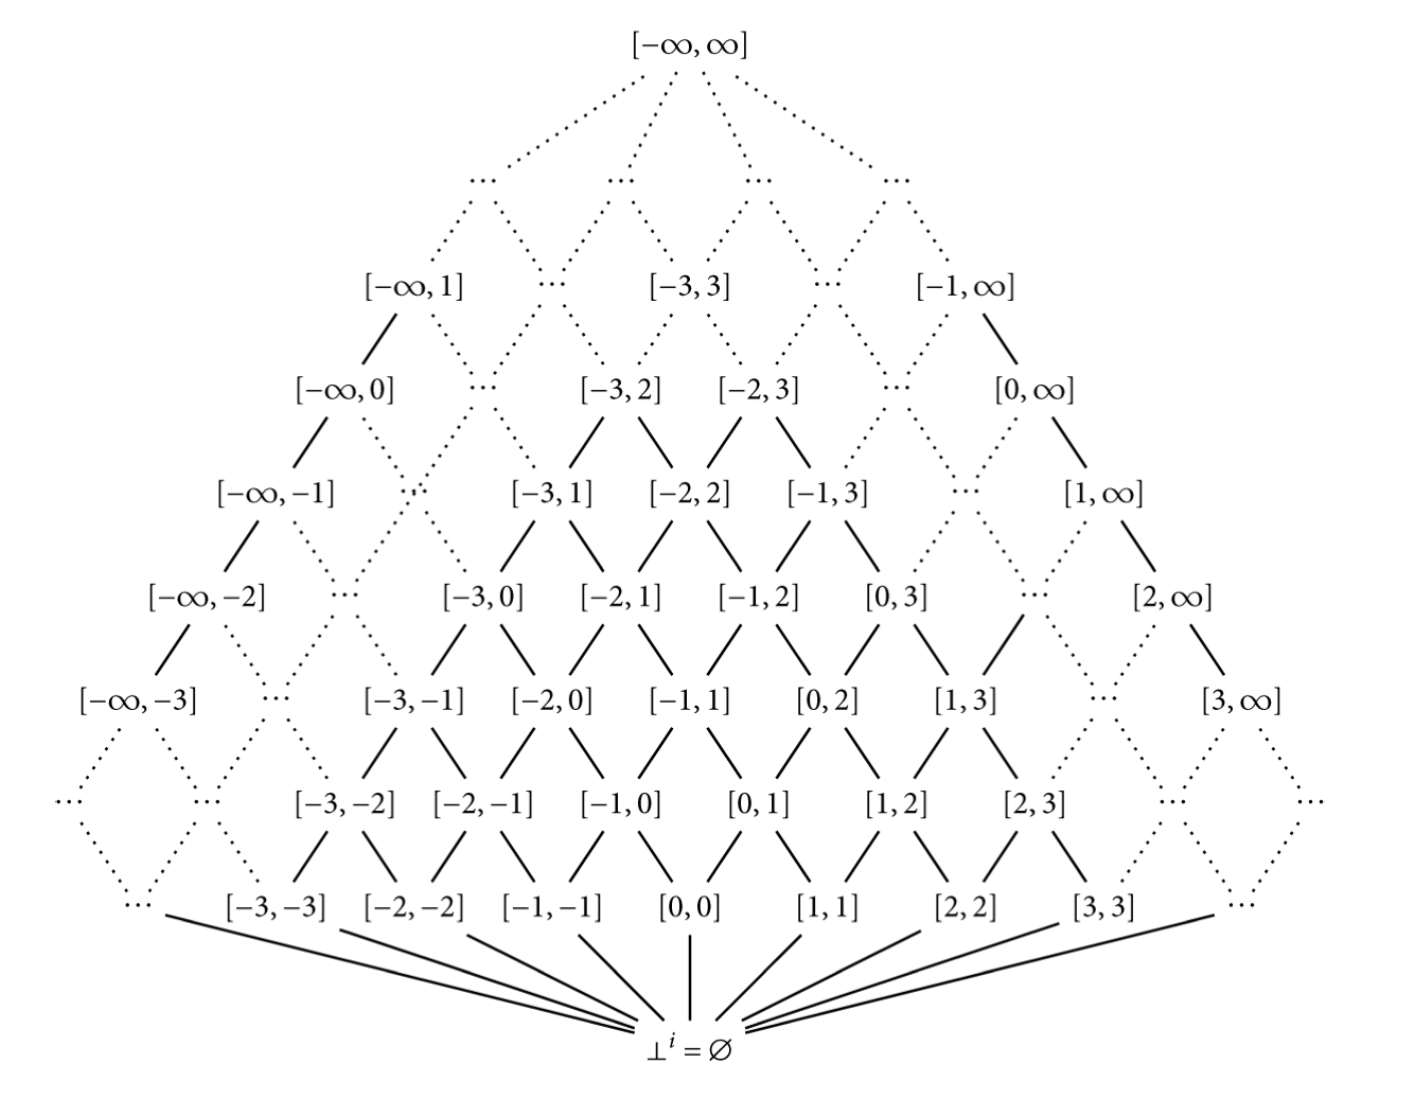
\includegraphics[width=0.7\textwidth]{images/interval_lattice.png}
    \caption[Caption for LOF]%
        {확장된 정수 구간도메인 $\mathbb{I}_{\mathbb{Z}_{\infty}}$}
    \label{fig:int_lattice}
\end{figure}

Boolean 값은 $\mathbf{true}, \mathbf{false}$ 만 존재하기에 요약도메인을 그림 \ref{fig:bool_domain}과 같이 정의할 수 있다.
$\top$ 의 경우 $\mathbf{true}, \mathbf{false}$ 가 모두 가능한 경우이마, $\bot$는 유효한 boolean 값 산출이 불가능한 경우이다.
\begin{figure}[t]
    \centering
    \begin{tikzpicture}[
    node distance=1cm,
    lattice/.style={},
    map/.style={->,blue,thick},
]

%----------------------------------
% Concrete lattice
%----------------------------------

\node[lattice] (cTop) {$\top$};

\node[lattice,below left=of cTop] (cTrue) {$\mathbf{true}$};
\node[lattice,below right=of cTop] (cFalse) {$\mathbf{false}$};

\node[lattice,below right=of cTrue] (cBot) {$\bot$};

\draw (cTop) -- (cTrue);
\draw (cTop) -- (cFalse);

\draw (cTrue) -- (cBot);
\draw (cFalse) -- (cBot);

\end{tikzpicture}
    \caption{Boolean 요약도메인}
    \label{fig:bool_domain}
\end{figure}

\subparagraph{제어 흐름 그래프(control-flow graph)} ~\\

간략화된 AST가 생성된 이후 \traceinspector는 \verb|if, while|등의 명령문에 의해 프로그램의 실행 흐름을 구조화하기 위한 제어 흐름 그래프(control-flow graph, CFG)구조\cite{alfred2007}로 번역한다.
함수별 AST에서 CFG를 생성하는 알고리즘은 다음과 같이 동작한다:
\begin{enumerate}
    \item 함수의 진입 명령문으로부터 깊이 우선 탐색을 통해 함수의 종말 명령문부터 노드로 번역하여 ID를 부여한다.
    \item 후속 노드의 DFS가 종료되면서 현재 노드와 이어줄 간선을 생성한다. 만약 현재 노드가 조건문, 반복문과 같이 분기를 포함하는 경우 각 참, 거짓 명령문별 노드와 간선을 생성해준다.
    \item \verb|break, continue|는 현재 동작하고 있는 가장 깊은 반복문에 대해 동작한다. 이를 처리하기 위해서 현재 처리중인 반복문을 스택 구조로 저장하여 중첩된 반복문에 대한 정보를 저장한다.
    \item 이에 따라 \verb|break, continue| 및 루프 탈출은 반복문 스택의 top에 대해 동작하며, 반복문을 처리 완료했다면 스택에서 반복문 정보를 제거한다.
\end{enumerate}

\begin{figure}[t]
    \centering
    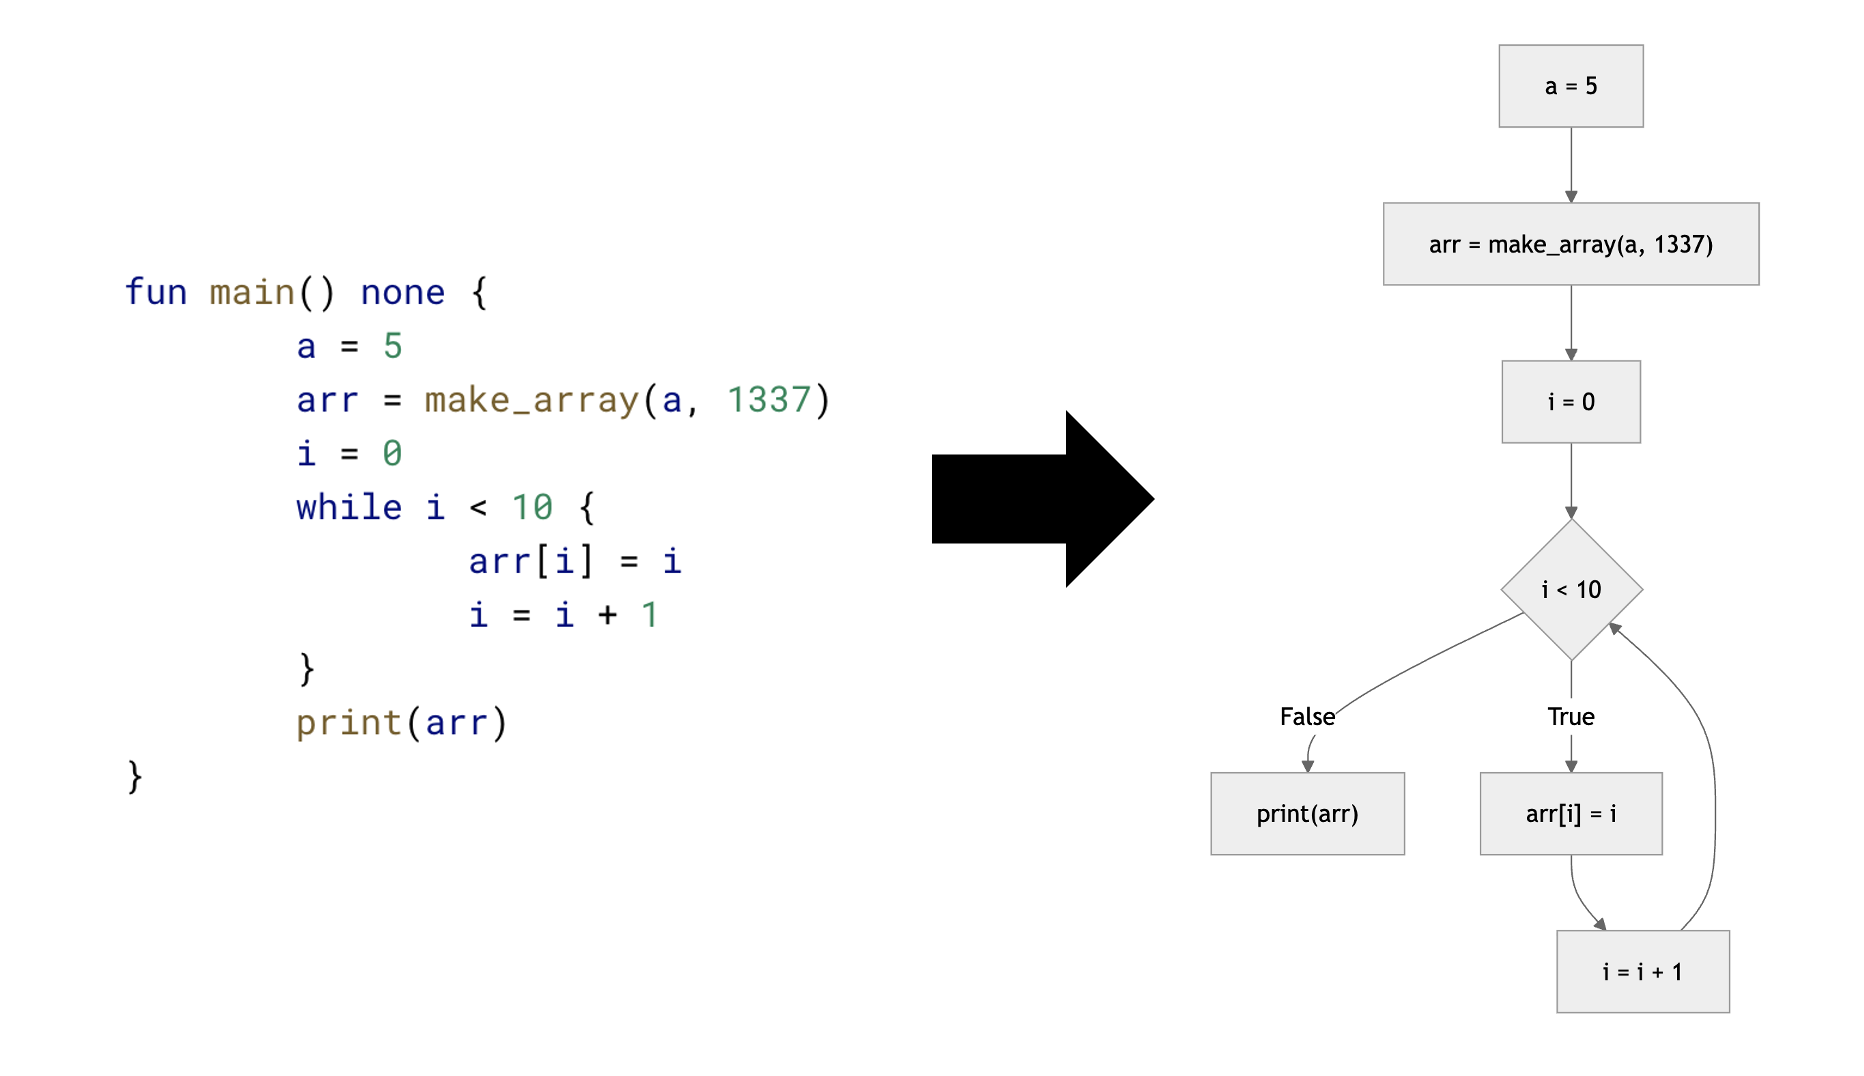
\includegraphics[width=0.9\textwidth]{images/imp2cfg.png}
    \caption{입력 \imp코드와 CFG로의 표현}
    \label{fig:imp2cfg}
\end{figure}

그림 \ref{fig:imp2cfg}는 예시 \imp 코드에 대한 CFG 표현 결과를 나타낸다. 각각의 명령문들이 단일 노드로 표현되며, \verb|while i < 10 {...}| 반복문을
\verb|i < 10| 조건을 하나의 단일 노드로 표현하고 판정 결과에 따라 후속 명령문들을 실행하는 형태로 나타낸 것을 확인할 수 있다.

이러한 CFG구조는 프로그램의 실행 흐름을 직접적으로 노출시키며, \verb|if, while, break, continue| 등의 문법적인 경우를 전부 열거할 필요 없이 조건 노드와 
참, 거짓 후속 노드에 대해서만 논할 수 있도록 분석을 간략하게 해준다. 
따라서 이후에 \traceinspector 분석기는 제어 흐름 그래프 위에서 직접적으로 동작하는 형태로 설계할 수 있으며, \imp 언어의 문법적 디테일로부터 보다 자유롭게 추상화된 형태로 동작이 가능하다.

\subparagraph{요약실행 의미론} ~\\

이제 입력 프로그램을 CFG 형태로 표현하여 분석이 수월한 형태의 자료구조로 번역하였다. 또한 \imp의 구체적인 값 타입들을 전부 각각의 요약도메인으로 대응시키는 $\alpha$ 함수도 정의하였다.

\imp의 구체적인 실행의미론에선 프로그램 상태 $\sigma : \mathbb{V} \rightarrow v$는 각 변수를 값으로 대응시켰다(부록 참조). 
또한 명령문 $S$를 프로그램 상태 $\sigma$에서 실행했을 때는 결과 상태 $\sigma'$와 제어 흐름 결과 $r$를 반환하며
$\langle S, \sigma \rangle \Downarrow \langle \sigma', r \rangle$로 표기했다.

\imp의 실제 실행이 구체적인 값 $\mathbb{V}$에 대해 계산을 하는 의미론에 바탕을 두었다면, 분석을 위해선 값들의 요약도메인 $A$ 위에서 실행되는 요약실행 의미론을 정의해야 한다.

요약실행 의미론에서 요약된 값은 $\mathsf{AbstractValue} : \tau \rightarrow v^{\#}_\tau$로 표현된다.
즉 타입 $\tau$를 해당 타입의 요약도메인 상애서의 값 $v^{\#}_\tau$로 대응하는 구조가 일차적으로 정의된다.

$\mathsf{AbstractValue}$는 각 변수마다 존재하기에, 주어진 프로그램 상태에서 각 변수 $v \in \mathbb{V}$를 각각의 $\mathsf{AbstractValue}$ 로 대응하는 $\mathsf{AbstractVarMemMap} : \mathbb{V} \rightarrow \mathsf{AbstractValue}$로 명령문을 실행하는 시점에서의 변수들의 요약 상태를 나타낸다.

이후 CFG 노드별 ID $l \in \mathbb{L}$를 $\mathsf{AbstractVarMemMap}$로 대응시키는 함수 단위의 대응 $\mathsf{AbstractNodeMemMap} : \mathbb{L} \rightarrow \mathsf{AbstractVarMemMap}$ 가 정의된다.
여기서 $\mathsf{AbstractValue}$는 노드 $l$에서 "해당 명령을 실행하기 전의 프로그램 상태", 즉 precondition 상태를 나타낸다.

최종적으로 프로그램 전체의 요약 메모리 상태는 입력 프로그램의 함수들 $f \in F$에서 함수별 요약 메모리 상태 $\mathsf{AbstractNodeMemMap}_f$로 대응하는 $\mathsf{AbstractFunctionMem} : F \rightarrow m^{\#}$로 나타낸다.

요약실행 의미론은 CFG 노드 $l$을 요약 메모리 상태 $M^{\#} : \mathsf{AbstractVarMemMap}$ 에서 실행했을 때 후속으로 실행할 CFG 노드 $l'$과 갱신된 요약 메모리 상태 $M^{\#'} : \mathsf{AbstractVarMemMap}$를 반환하는
단일 실행 단계로 표현할 수 있으며, $(l, M^\#) \hookrightarrow^{\#} (l', M^{\#'})$로 표기한다.

이후 $l'$에 대한 갱신된 요약 프로그램 상태 $M^{\#'}$과 기존에 계산된 요약 프로그램 상태 $\mathsf{AbstractNodeMemMap}(l')$과의 join연산 $M^{\#'} \sqcup \mathsf{AbstractNodeMemMap}(l')$을 수행하여 $l'$의 상태를 갱신한다.

따라서 요약 실행 알고리즘은 다음과 같이 설명할 수 있다:
\begin{enumerate}
    \item 주어진 함수 $f$에 대한 초기 상태 $S : \mathsf{AbstractVarMemMap}$ 와 진입 노드 $l_{\mathsf{init}}$가 주어졌을 때 $(l_{\mathsf{init}}, S) \hookrightarrow^{\#} (l', M^{\#'})$을 계산
    \item 기존의 $\mathsf{AbstractNodeMemMap}(l')$를 $\mathsf{AbstractNodeMemMap}(l') \sqcup M^{\#'}$로 갱신
    \item 이후 $l'$ 에서 바로 도달 가능한 후속 노드들 $next(l')$에 대해 위 과정을 반복해서 수행
 \end{enumerate}

위 알고리즘은 초기 프로그램 상태에서부터 각 노드에 대해 요약실행 의미론을 적용하여 노드별 상태를 계속해서 갱신하고, 더 이상 변화가 생기지 않는 \textbf{고정점}에 도달할 때 까지 반복 수행한다. 
이렇게 계산된 고정점 프로그램 상태는 각 노드에서 관측 가능한 모든 값에 대한 정보가 반영된 프로그램 상태이며, 실제로 실행했을 때의 모든 값을 포함한 보수적인 근사 상태가 된다. 
컴파일러가 data-flow analysis를 수행할 때 활용하는 Kildall 알고리즘\cite{kildall1973}처럼 CFG위에서 노드별 상태를 계산하는 과정이 유사하다.

그림 \ref{fig:abs_conc_commute}은 요약 실행의미론과 구체적 실행의미론의 관계를 묘사한다. 
앞서 설명한 보수적인 근사가 성립하기 위해선, 요약 메모리 상태 $M^{\#}$가 모든 명령문에 대해 $M^{\#'}$로 요약실행이 된다면, $M^{\#}$의 구체적 상태 $\sigma = \gamma(M^{\#})$에 대해 실제로 실행했을 때 얻는 상태 $\sigma'$는 
 $M^{\#'}$의 구체적 상태 $\gamma(M^{\#'})$ 포함되어 있어야 한다.\footnote{보다 엄밀한 정의는 메모리 상태 $\mathbb{V}$의 각 변수에 $v$에 대한 pointwise-lifted 명세로 정의한다: $\forall v \in \mathbb{V}. \sigma[v] \in \gamma(M^{\#}[v])$}

\begin{figure}[t]
    \centering
    % https://q.uiver.app/#q=WzAsNCxbMCwwLCJNXntcXCN9IDogXFxtYXRoc2Z7QWJzdHJhY3RWYXJNYXB9Il0sWzIsMCwiTV57XFwjJ30gOiBcXG1hdGhzZntBYnN0cmFjdFZhck1hcH0iXSxbMCwyLCJcXHNpZ21hIDogXFxtYXRoYmJ7Vn0gXFxyaWdodGFycm93IHYiXSxbMiwyLCJcXHNpZ21hJyA6IFxcbWF0aGJie1Z9IFxccmlnaHRhcnJvdyB2Il0sWzAsMSwiXFxob29rcmlnaHRhcnJvd157XFwjfSJdLFsyLDMsIlxcRG93bmFycm93Il0sWzAsMiwiXFxnYW1tYSIsMV0sWzEsMywiXFxnYW1tYSIsMV1d
\[\begin{tikzcd}
	{M^{\#} : \mathsf{AbstractVarMap}} && {M^{\#'} : \mathsf{AbstractVarMap}} \\
	\\
	{\sigma : \mathbb{V} \rightarrow v} && {\sigma' : \mathbb{V} \rightarrow v}
	\arrow["{\hookrightarrow^{\#}}", from=1-1, to=1-3]
	\arrow["\gamma"{description}, from=1-1, to=3-1]
	\arrow["\gamma"{description}, from=1-3, to=3-3]
	\arrow["\hookrightarrow", from=3-1, to=3-3]
\end{tikzcd}\]
    \caption{요약 실행단계 $\hookrightarrow^{\#}$와 구체적 실행단계 $\hookrightarrow$과의 대응}
    \label{fig:abs_conc_commute}
\end{figure}

위 과정을 그대로 실행할 경우 잠재적으로 끝나지 않는 프로그램(무한루프가 포함된 프로그램 등)의 경우 고정점에 도달할 수 없기에 분석도 종료되지 않는다. 
이는 $M^{\#}$에서 사용되는 요약도메인의 높이가 무한한 경우 새로 갱신되는 $\mathsf{AbstractNodeMemMap}(l') \sqcup M^{\#'}$가 계속해서 증가하기 때문이다. 따라서 무한히 증가하는 요약상태에 대한 고정점을 제공하는
widening 연산 $\mathsf{AbstractNodeMemMap}(l') \triangledown M^{\#'}$을 적용하여 고정점에 도달할 수 있도록 유도해야 한다. 
\traceinspector에서 사용한 요약 도메인 중 정수 구간 도메인과 배열 배열 축약 도메인은 그 높이가 무한하기에, 위에서 정의한 widening을 적용하여 분석이 유한한 시간 내에 종료하도록 보장하였다.

최종적으로 \traceinspector에 대한 논리적 건전성을 다음과 같이 정의할 수 있다:

\begin{utheorem}[\traceinspector 분석기의 논리적 건전성]
	\imp의 모든 프로그램 $s$와 초기 프로그램 상태 $\sigma$에 대해, $M^{\#'} = analyze(s, \sigma)$를 \traceinspector 분석기가 계산한 최종 요약 고정점이라 하자.
    이때 $s$를 $\sigma$에서 실행했을 때 도달 가능한 모든 구체적 프로그램 상태 $\sigma'$에 대해
    $$
    \sigma' \in \gamma(M^{\#'})
    $$
    가 성립힌다.
\end{utheorem}
증명은 각 요약도메인과 타입에 대한 갈루아 연결을 보인 후 \imp의 명령문에 대한 구조적 귀납으로 실시한다. 

이 증명은 \traceinspector의 분석 결과가 주어진 요약 의미론과 요약 도메인이 정의된 구체적 실행의미론에 대한 정확한 근사를 항상 취한다는 것을 보장한다.

\subparagraph{오류 상태 판별} ~\\

계산된 요약 상태 위에서 \traceinspector 분석기는 두가지 오류 조건을 검사한다. 
첫번째는 배열 인덱싱 \verb|a[i]| 가 주어졌을 때 가능한 모든 $i$의 값들이 $a$의 잠재적인 길이보다 작은지, 그리고 0보다 큰지 검사한다.
해당 검사는 요약 도메인상에서 실시하며 보수적인 추정이기 때문에 올바른 인덱싱임을 판정하면 모든 $a$와 $i$의 값에 대해 안전하지만, 반대로 오류가 나지 않을 \verb|a[i]|에 
대해서도 오류가 발생할 수 있음을 알리게 된다.

두번째 오류 상태는 CFG의 조건 노드에 대해 수행하며, 조건식의 요약도메인 계산값이 $\top$ 이 아닌 $\mathrm{true, false}, \bot$인 경우 경고를 한다.
조건식의 요약 결과가 $\top$인 경우 특정 입력들에 대해서는 참 혹은 거짓임을 나타내기에 즉각적으로 조건식의 결과에 대해 알 수 없게 된다. 하지만 요약 고정점 상태에서 
결과가 참 또는 거짓인 경우 해당 조건식에 도달했을 때 가능한 모든 값에 대해 참 또는 거짓으로 계산됨을 나타내므로 조건식 자체가 항진명제 혹은 모순명제가 되어 특정 분기가 도달 불가능함을 함의한다.


\paragraph{\textsf{TraceInspector} 프론트엔드} ~\\

\traceinspector 분석기가 위와 같은 이론을 바탕으로 결과값을 내뱉어 준다.
하지만, 이 상태 만으로, 프로젝트가 추구하는 "알고리즘 시각화"라는 개념을 실현하기는 힘들다.
따라서, 분석기와 연계하여 분석기의 출력을 정의하고 그를 바탕으로 UI와 실효 기능을 만들게 되었다.

프론트엔드 개발의 다음과 같은 원칙(Code of Conduct)을 적용하였으며, 이를 최상위로 추구한다. 

1. 복잡한 구조보다는 프로젝트가 추구하는 바를 실현하기 위해, KISS(Keep It Simple and Stupid) 철학을 준수한다.
2. 프론트엔드가 분석기인 만큼, 절대적인 안정성과 코드의 배포성을 지키기 위해 불필요한 라이브러리 사용은 지양한다.
3. 기능은 물론이고, 사소한 디자인 또한 모든 브라우저에서 동일하게 적용함을 원칙으로 한다.

\subparagraph{UI 요약설명} ~\\

\begin{figure}[H]
    \centering
    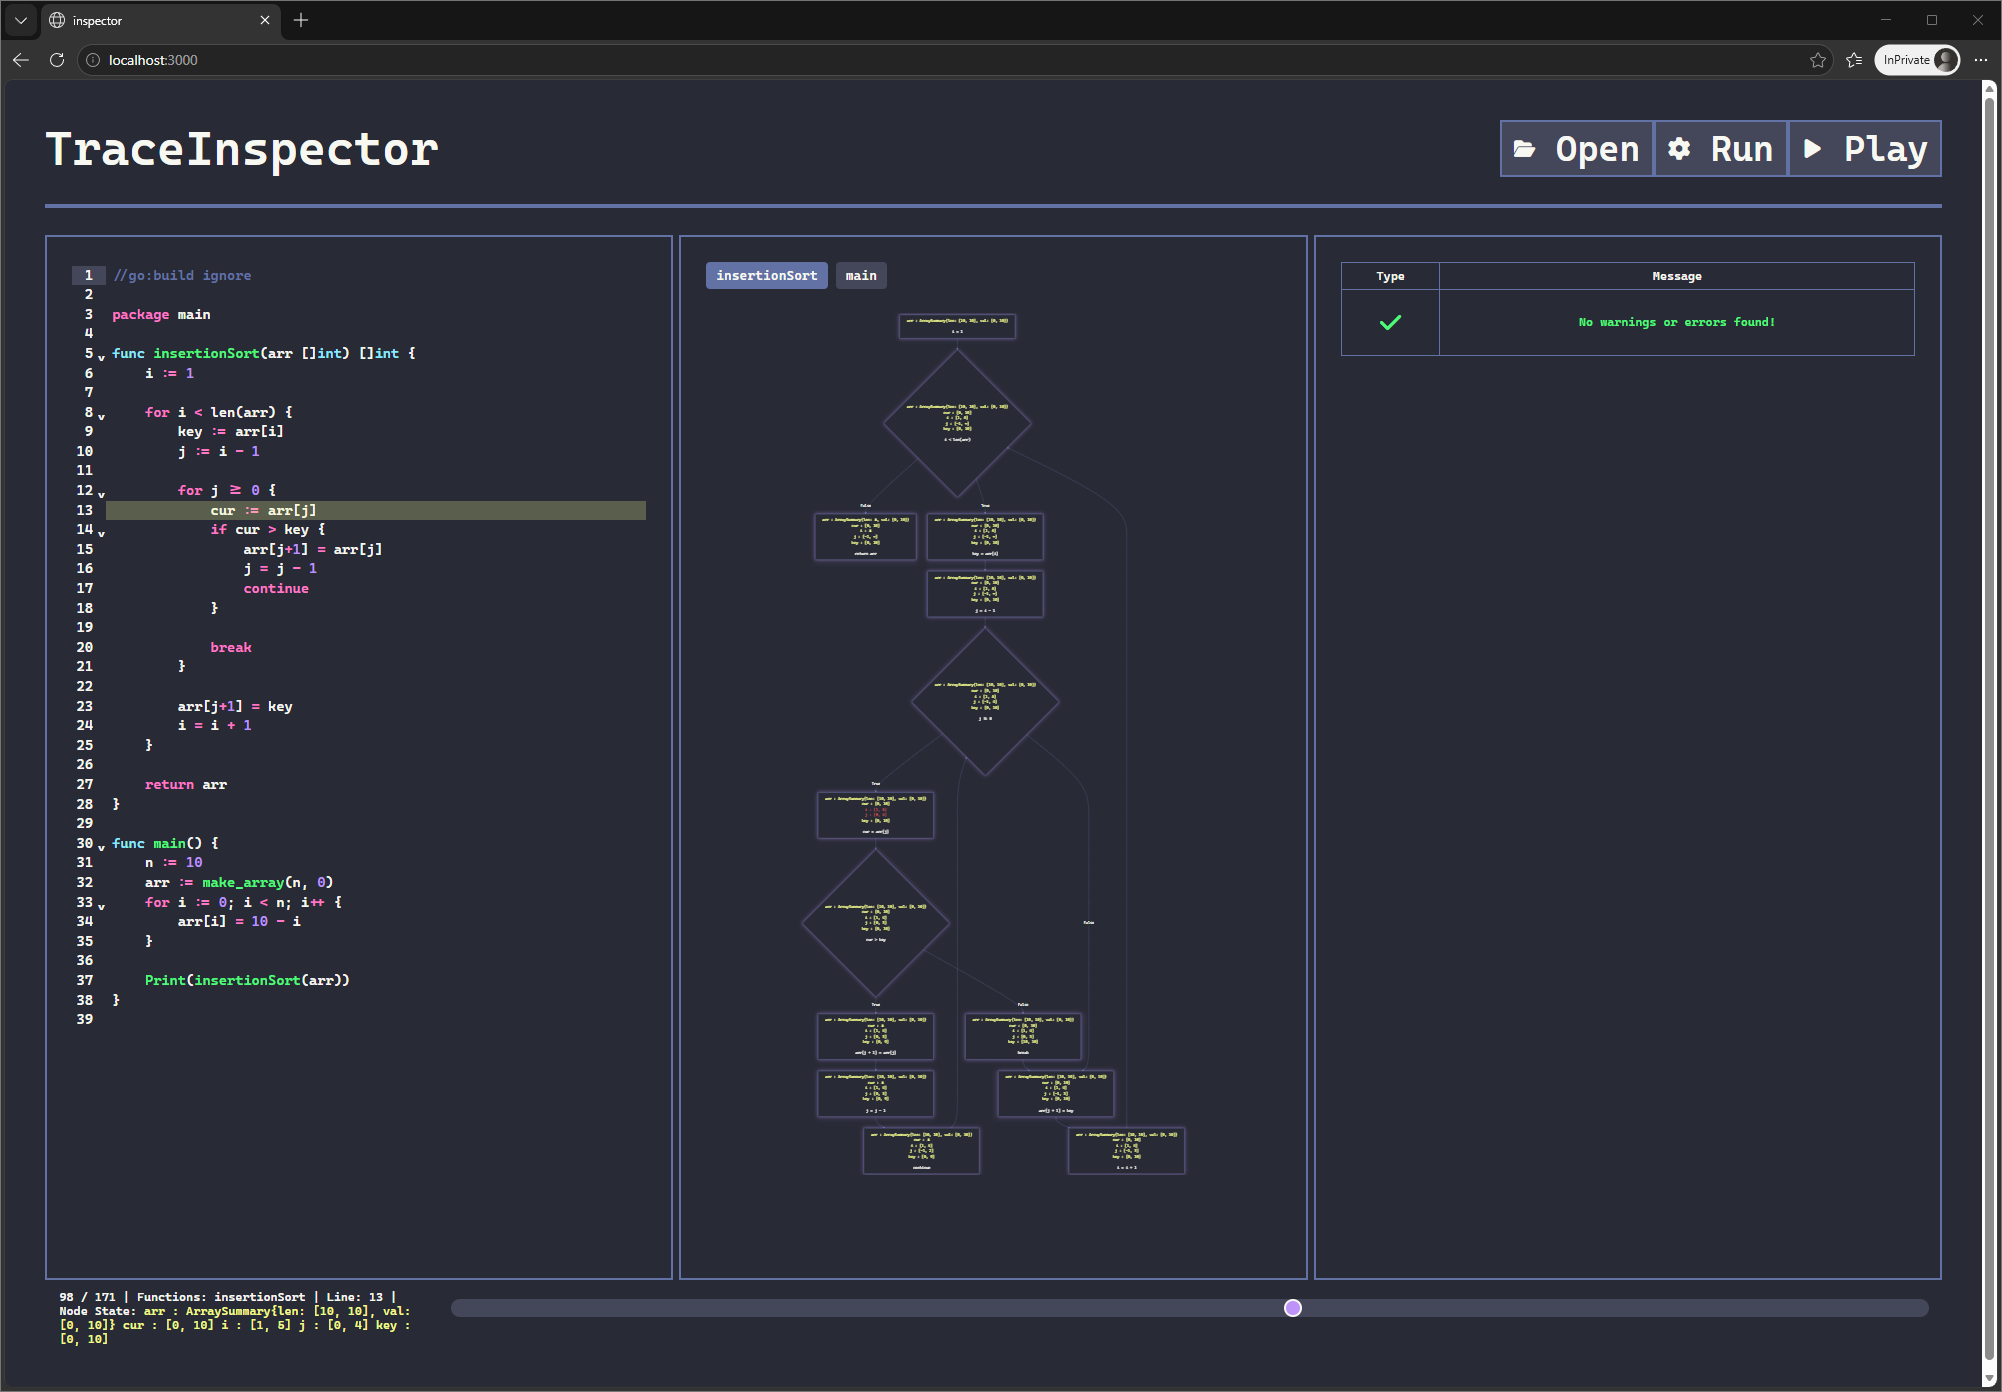
\includegraphics[width=0.8\textwidth]{images/front/00.jpg}
    \caption{전체 UI 구조}
\end{figure}

프론트엔드 UI는 "React-tRace"와 유사하게 제작 되었으며, 추가 설명은 다음 소제목에서 다루겠다.

상단에는 분석기 조작버튼이 존재하며, 각각 파일 입력, 분석 개시, 자동 재생 기능으로 구성되어 있다.
중간에는 각각 소스코드의 내용을 띄워주는 창, 분석한 그래프를 띄워주는 창, 분석기가 잡은 오류나 경고를 띄우는 창으로 구성되어 있다.
하단에는 분석기가 분석한 과정을 미디어 플레이어 처럼 조작하여 확인할 수 있는 슬라이더 바가 존재하며, 방향키나 드래그, 자동 재생 기능으로 제어할 수 있다.

\subparagraph{작동방식 상세설명} ~\\

\begin{figure}[H]
    \centering
    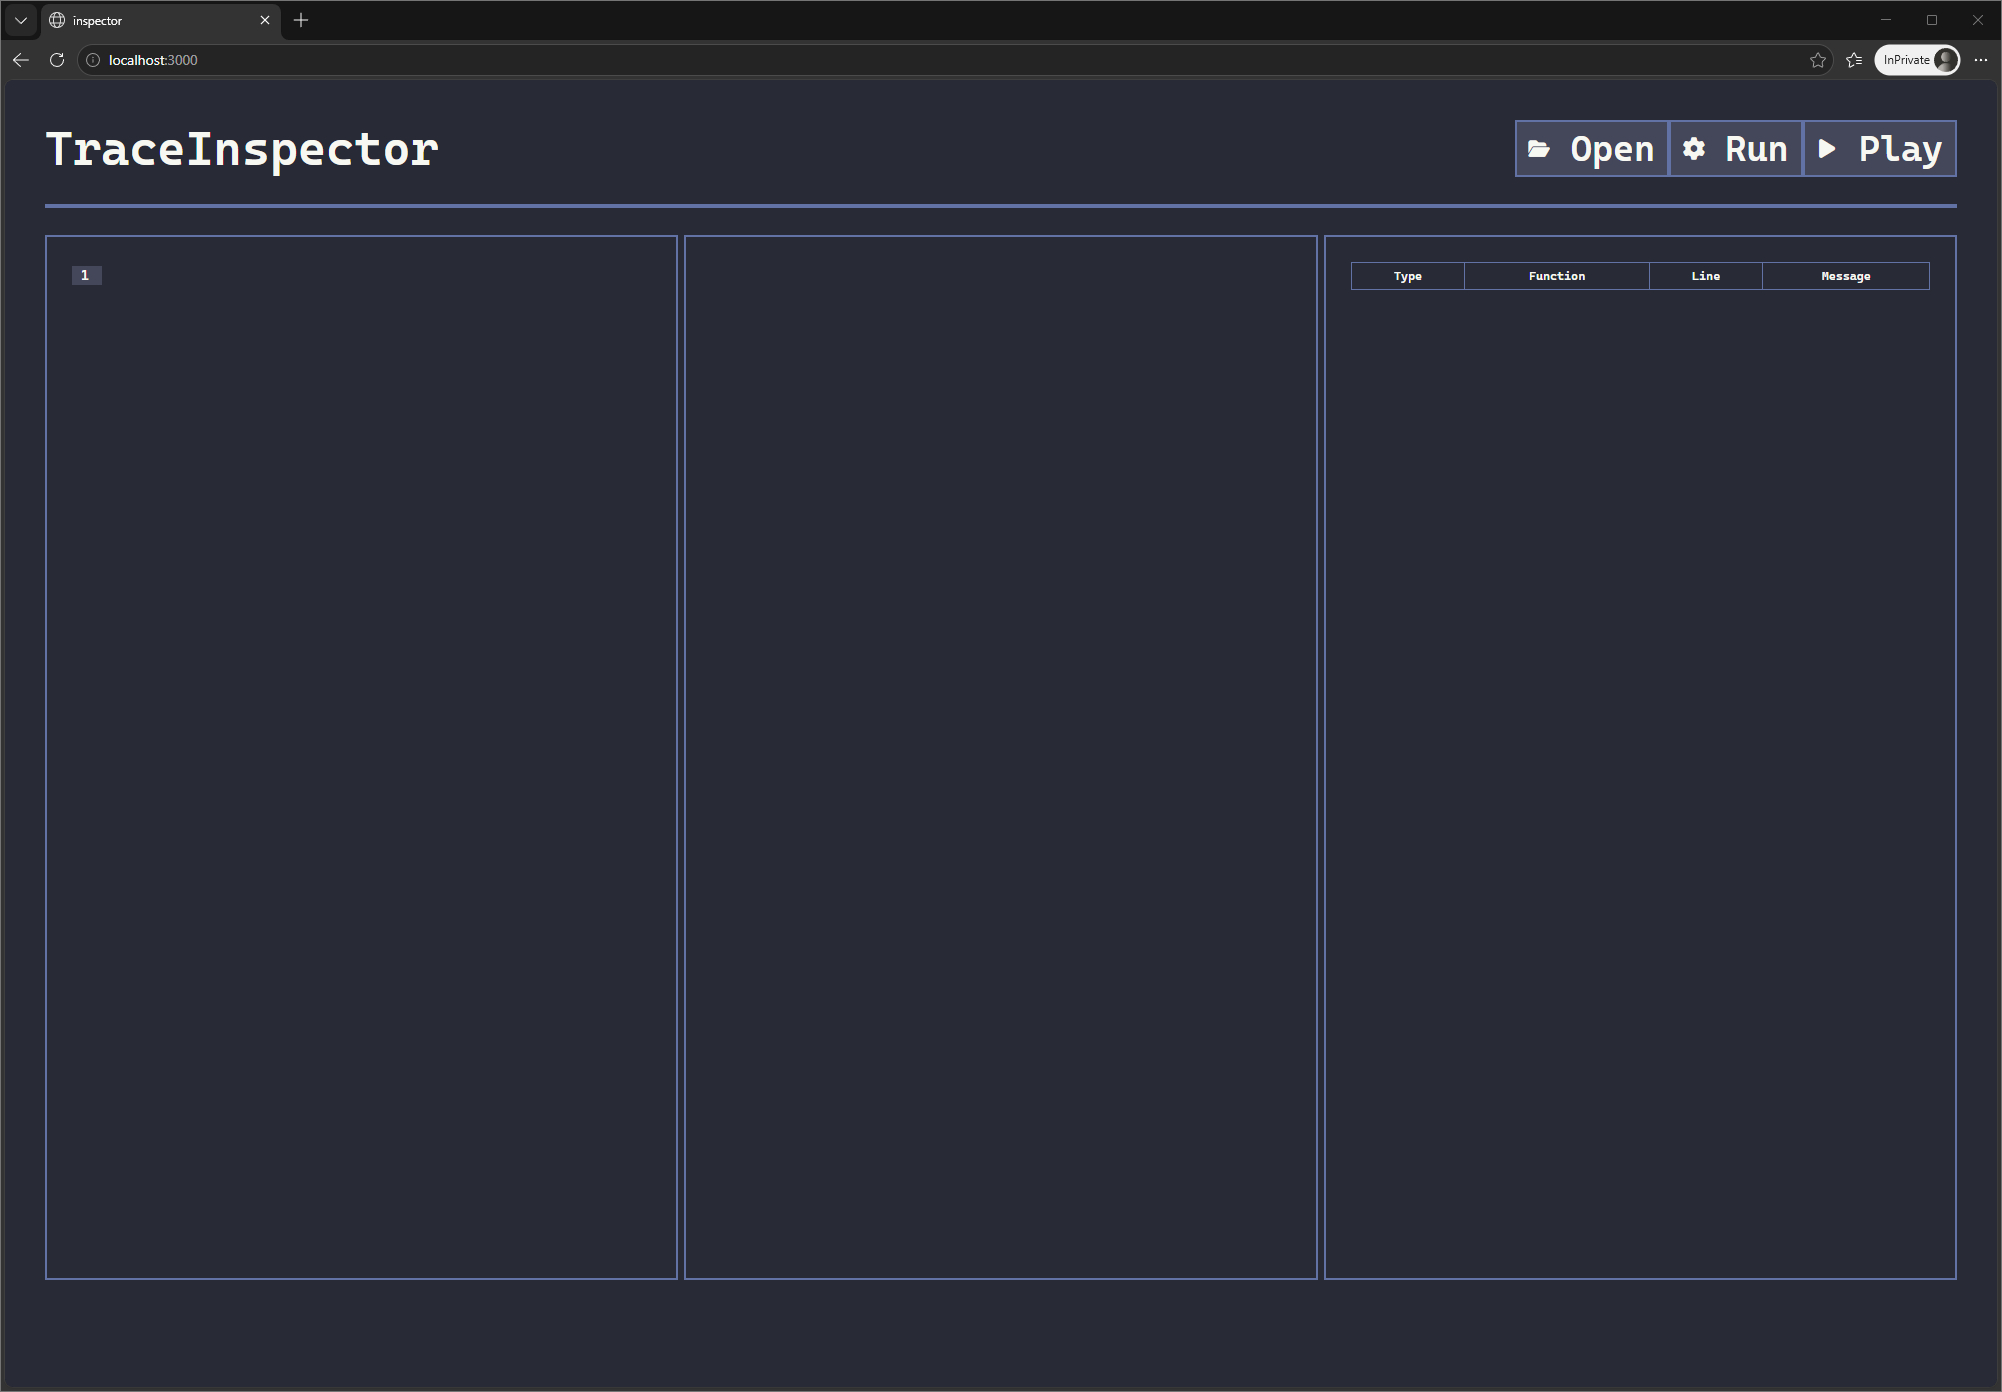
\includegraphics[width=0.8\textwidth]{images/front/01.jpg}
    \caption{초기 UI}
\end{figure}

프론트엔드를 실행하면 위와 같은 창이 생성이 된다. 
여기서 "Open" 버튼을 눌러 Go 소스코드를 불러온다.

위 기능을 위해, HTML의 기본으로 내장되어 있는 파일 입력을 사용하였고,
파일 입력이 성공하면, 왼쪽 코드 창에 출력한다.

\begin{figure}[H]
    \centering
    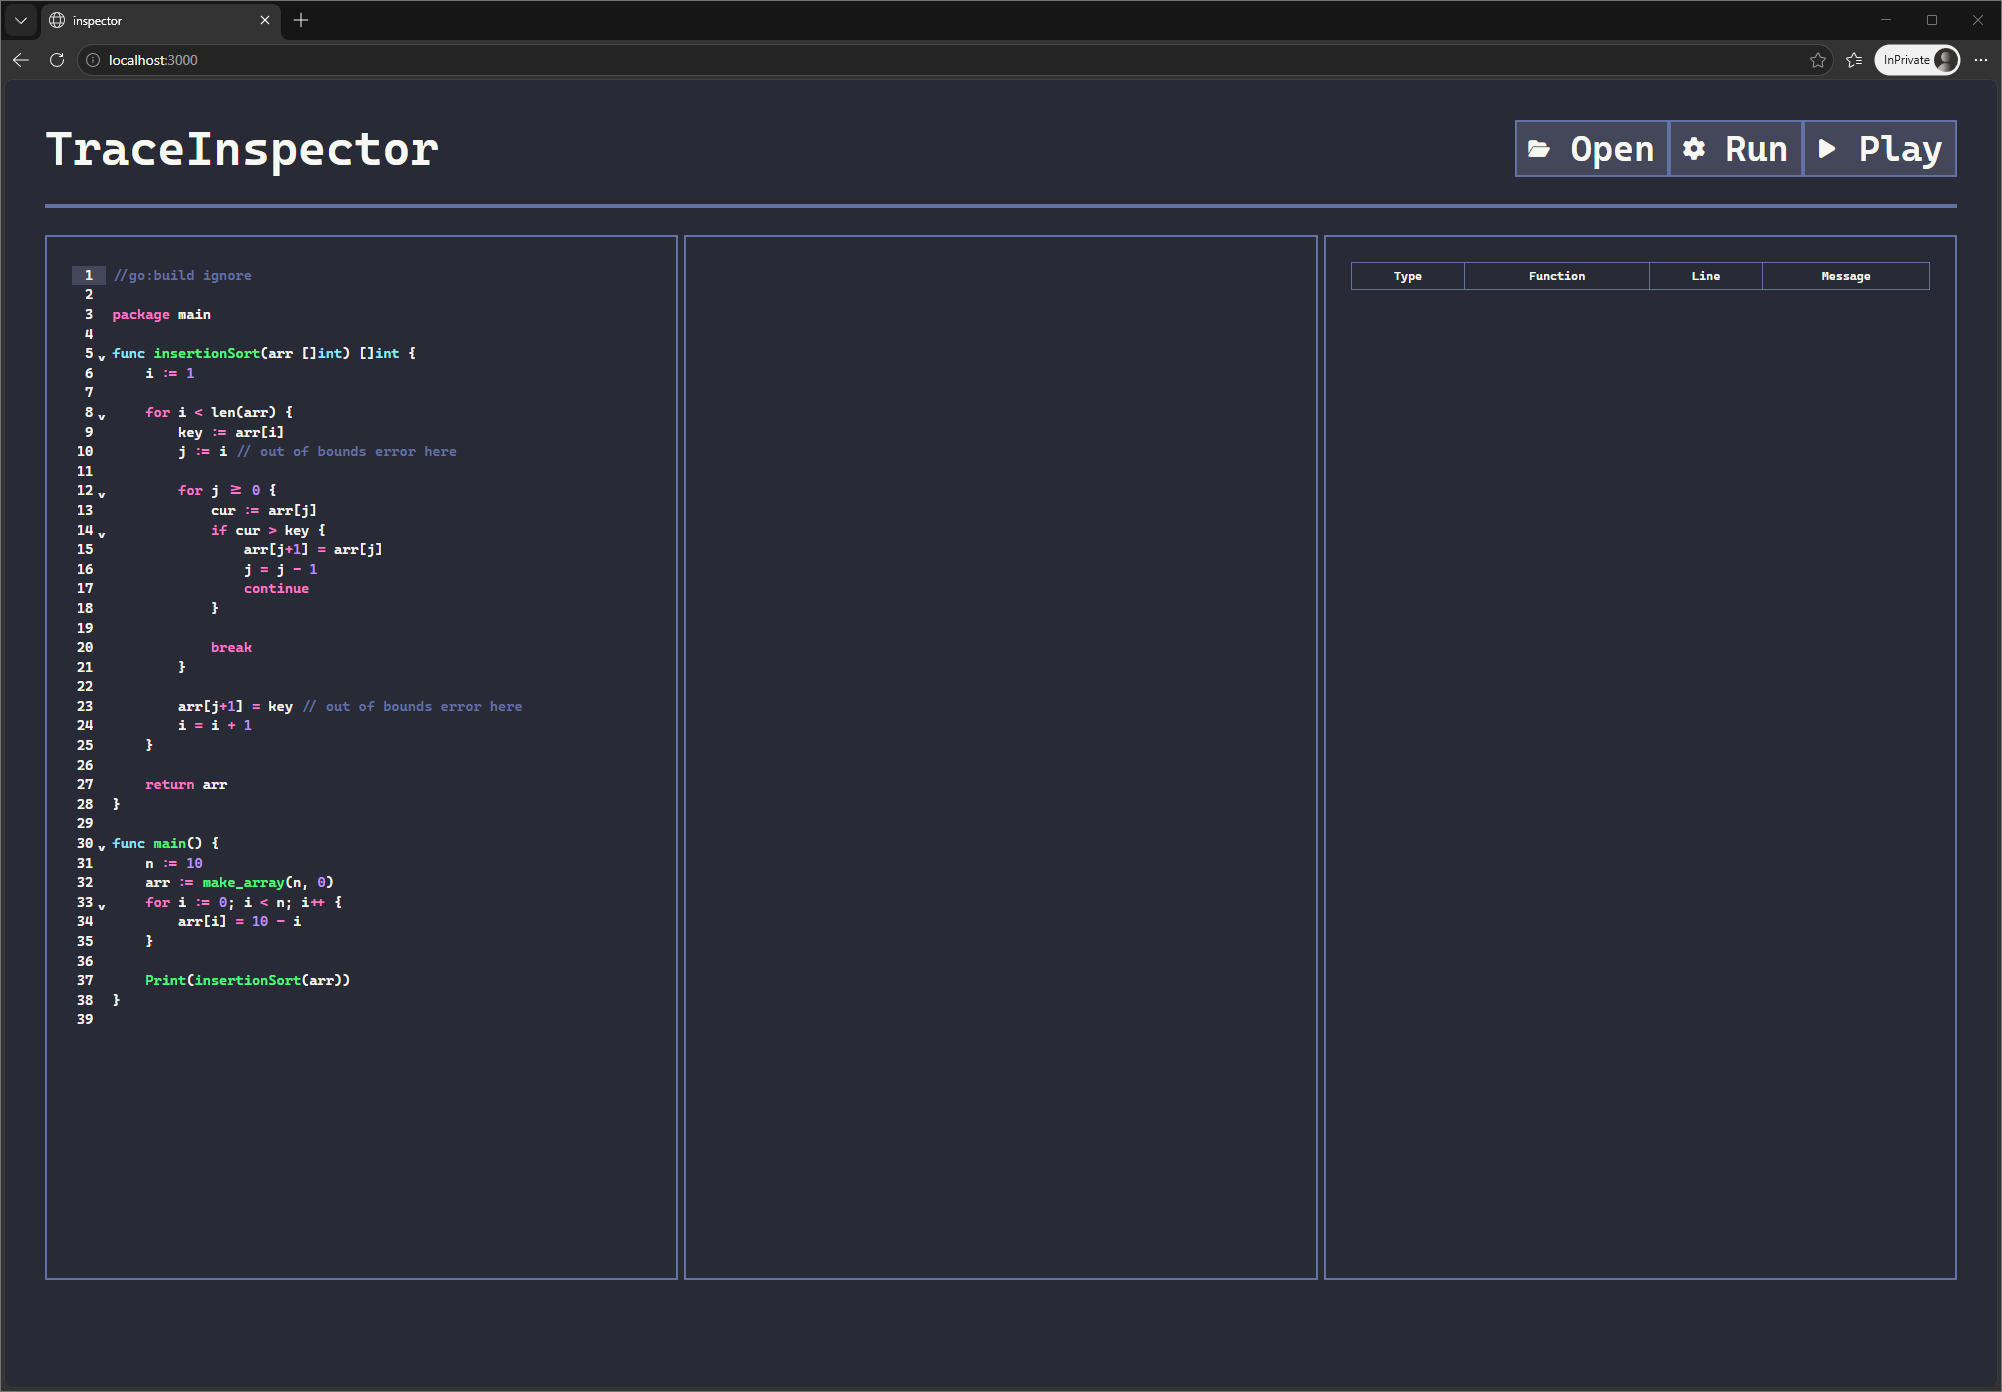
\includegraphics[width=0.8\textwidth]{images/front/02.jpg}
    \caption{Open 이후 UI}
\end{figure}

다음으로, 분석을 위해 "Run" 버튼을 누르게 되면, 입력 되어 있는 소스코드가 \\ \verb|front_src/go/source.go| 경로에 저장된다.
이때, "Multer" 라이브러리를 이용하여 파일 시스템에 직접적으로 출력하고, 이 과정을 ExpressJS로 제작한 서버에 /upload 신호로 넘겨 처리한다.

\begin{figure}[H]
    \centering
    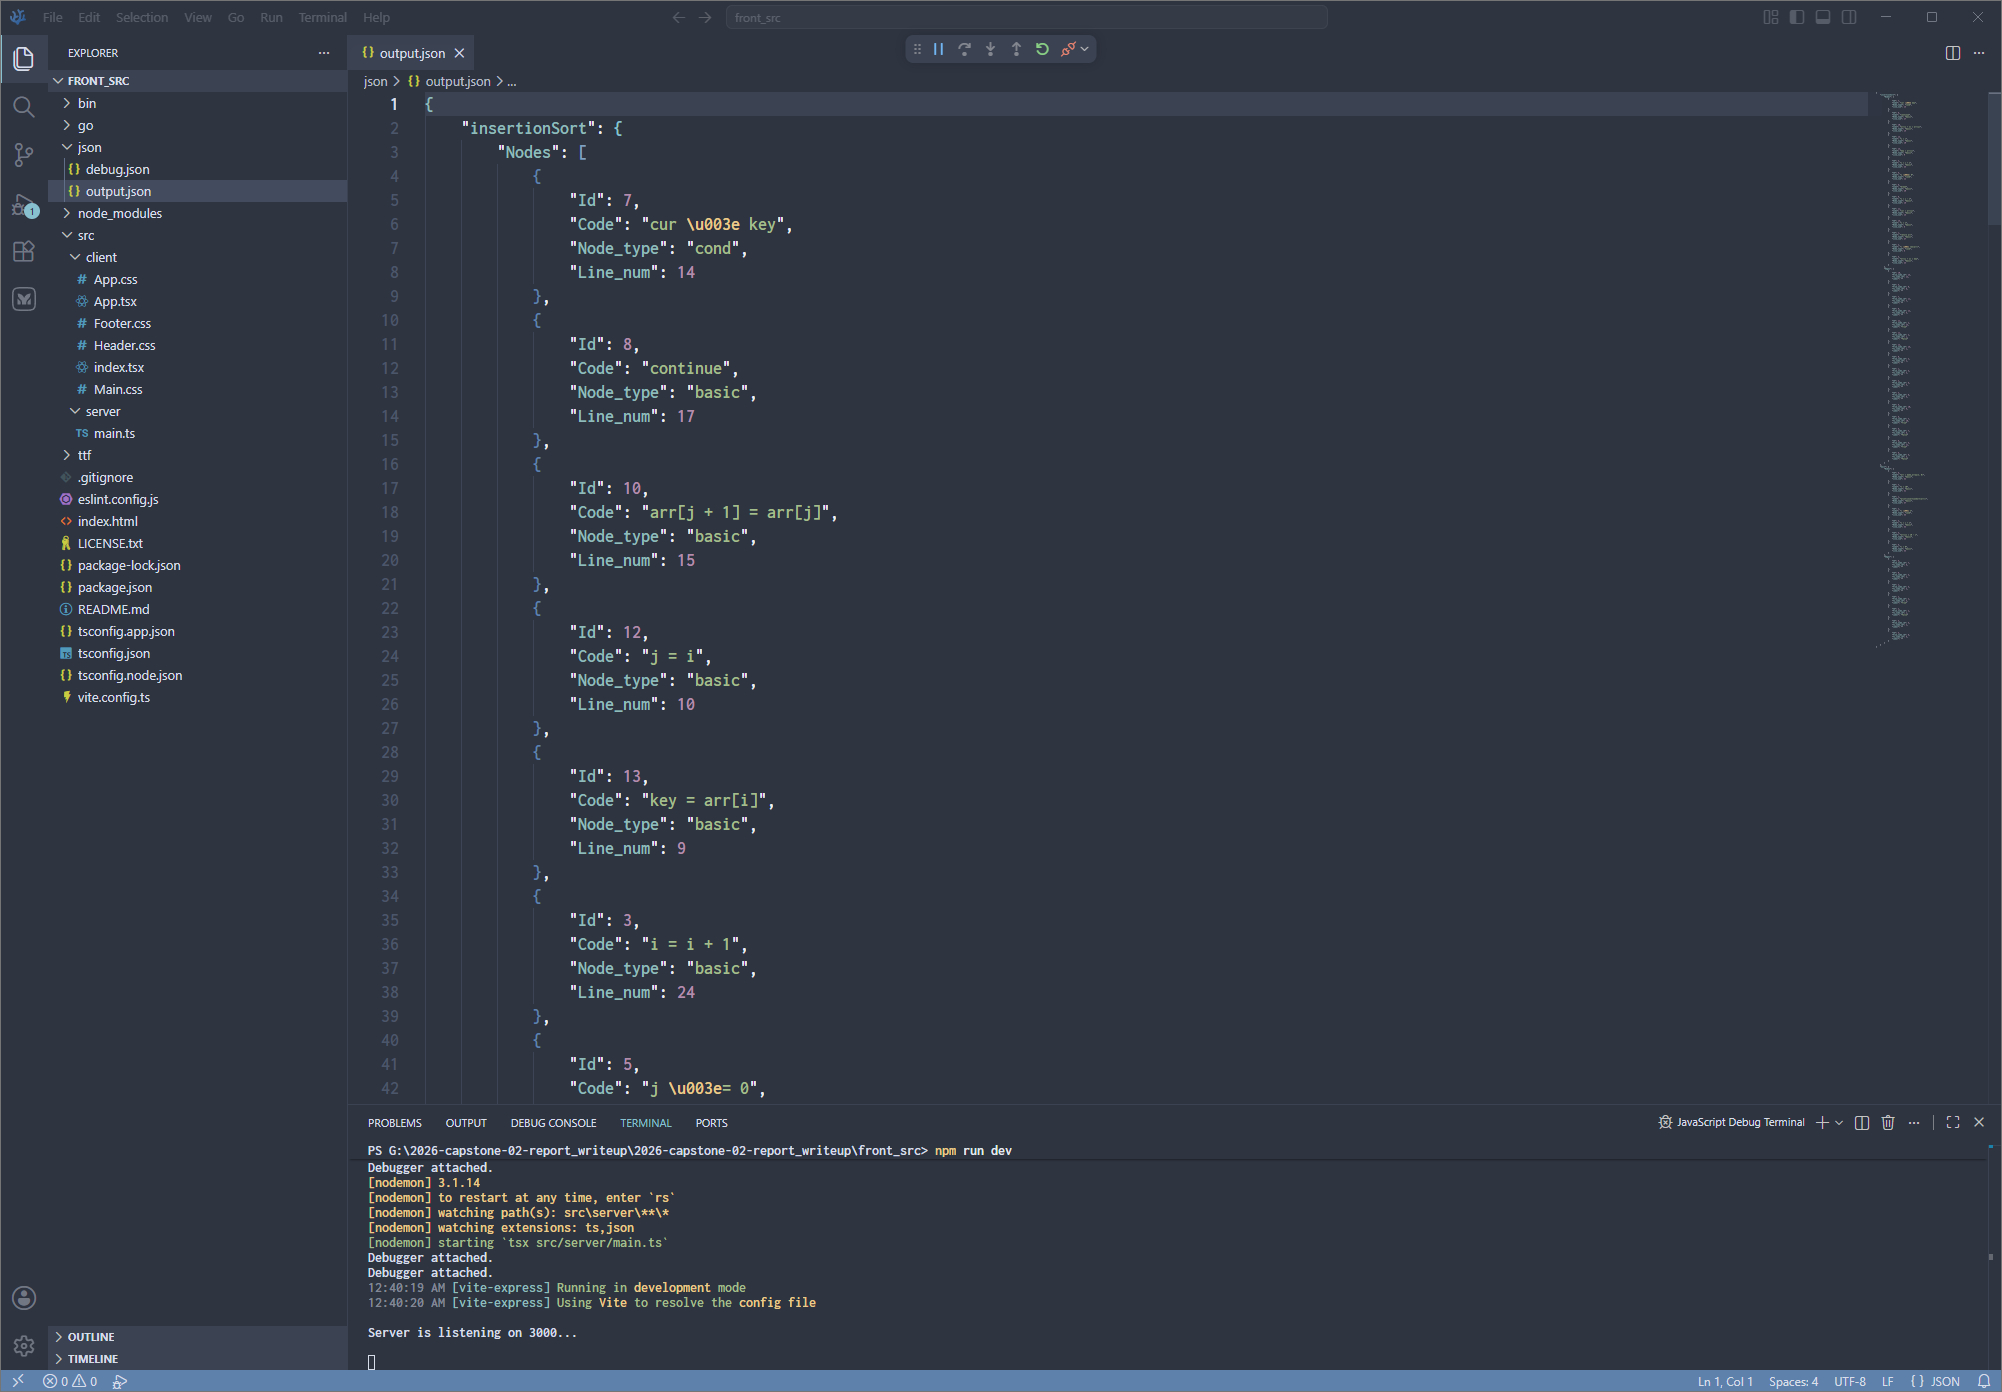
\includegraphics[width=0.8\textwidth]{images/front/03.jpg}
    \caption{1차 그래프 JSON 파일}
\end{figure}

처리가 완료가 되면, \verb|front_src/go/source.go|를 이용하여 분석기를 돌리고, 이 과정은 NodeJS 라이브러리 \verb|child_process| 내에 있는 \verb|exec| 함수를 이용한다.
분석기를 돌리면 분석기의 분석 과정이 생략된 1차 그래프 생성을 위한 JSON 파일이 \\ \verb|front_src/json/output.json| 생성된다. 추후에 변형을 가할 때 용이하도록 분리해 놓은 것이다.
이 과정을 ExpressJS로 제작한 서버에 /run 신호로 넘겨 처리하고 ReactJS 클라이언트로 복귀한다.

이후, 분석 과정이 생략된 경우를 감안하여 1차로 MermaidJS 그래프를 생성하여, 가운데 그래프 화면에 띄워준다.
이 과정에서, 향후 분석 과정을 각 그래프의 적용해야 하기 때문에 \verb|Mermaid_t|와 그 하위 클래스를 만들어 인스턴스로 저장하여준다.

\begin{figure}[H]
    \centering
    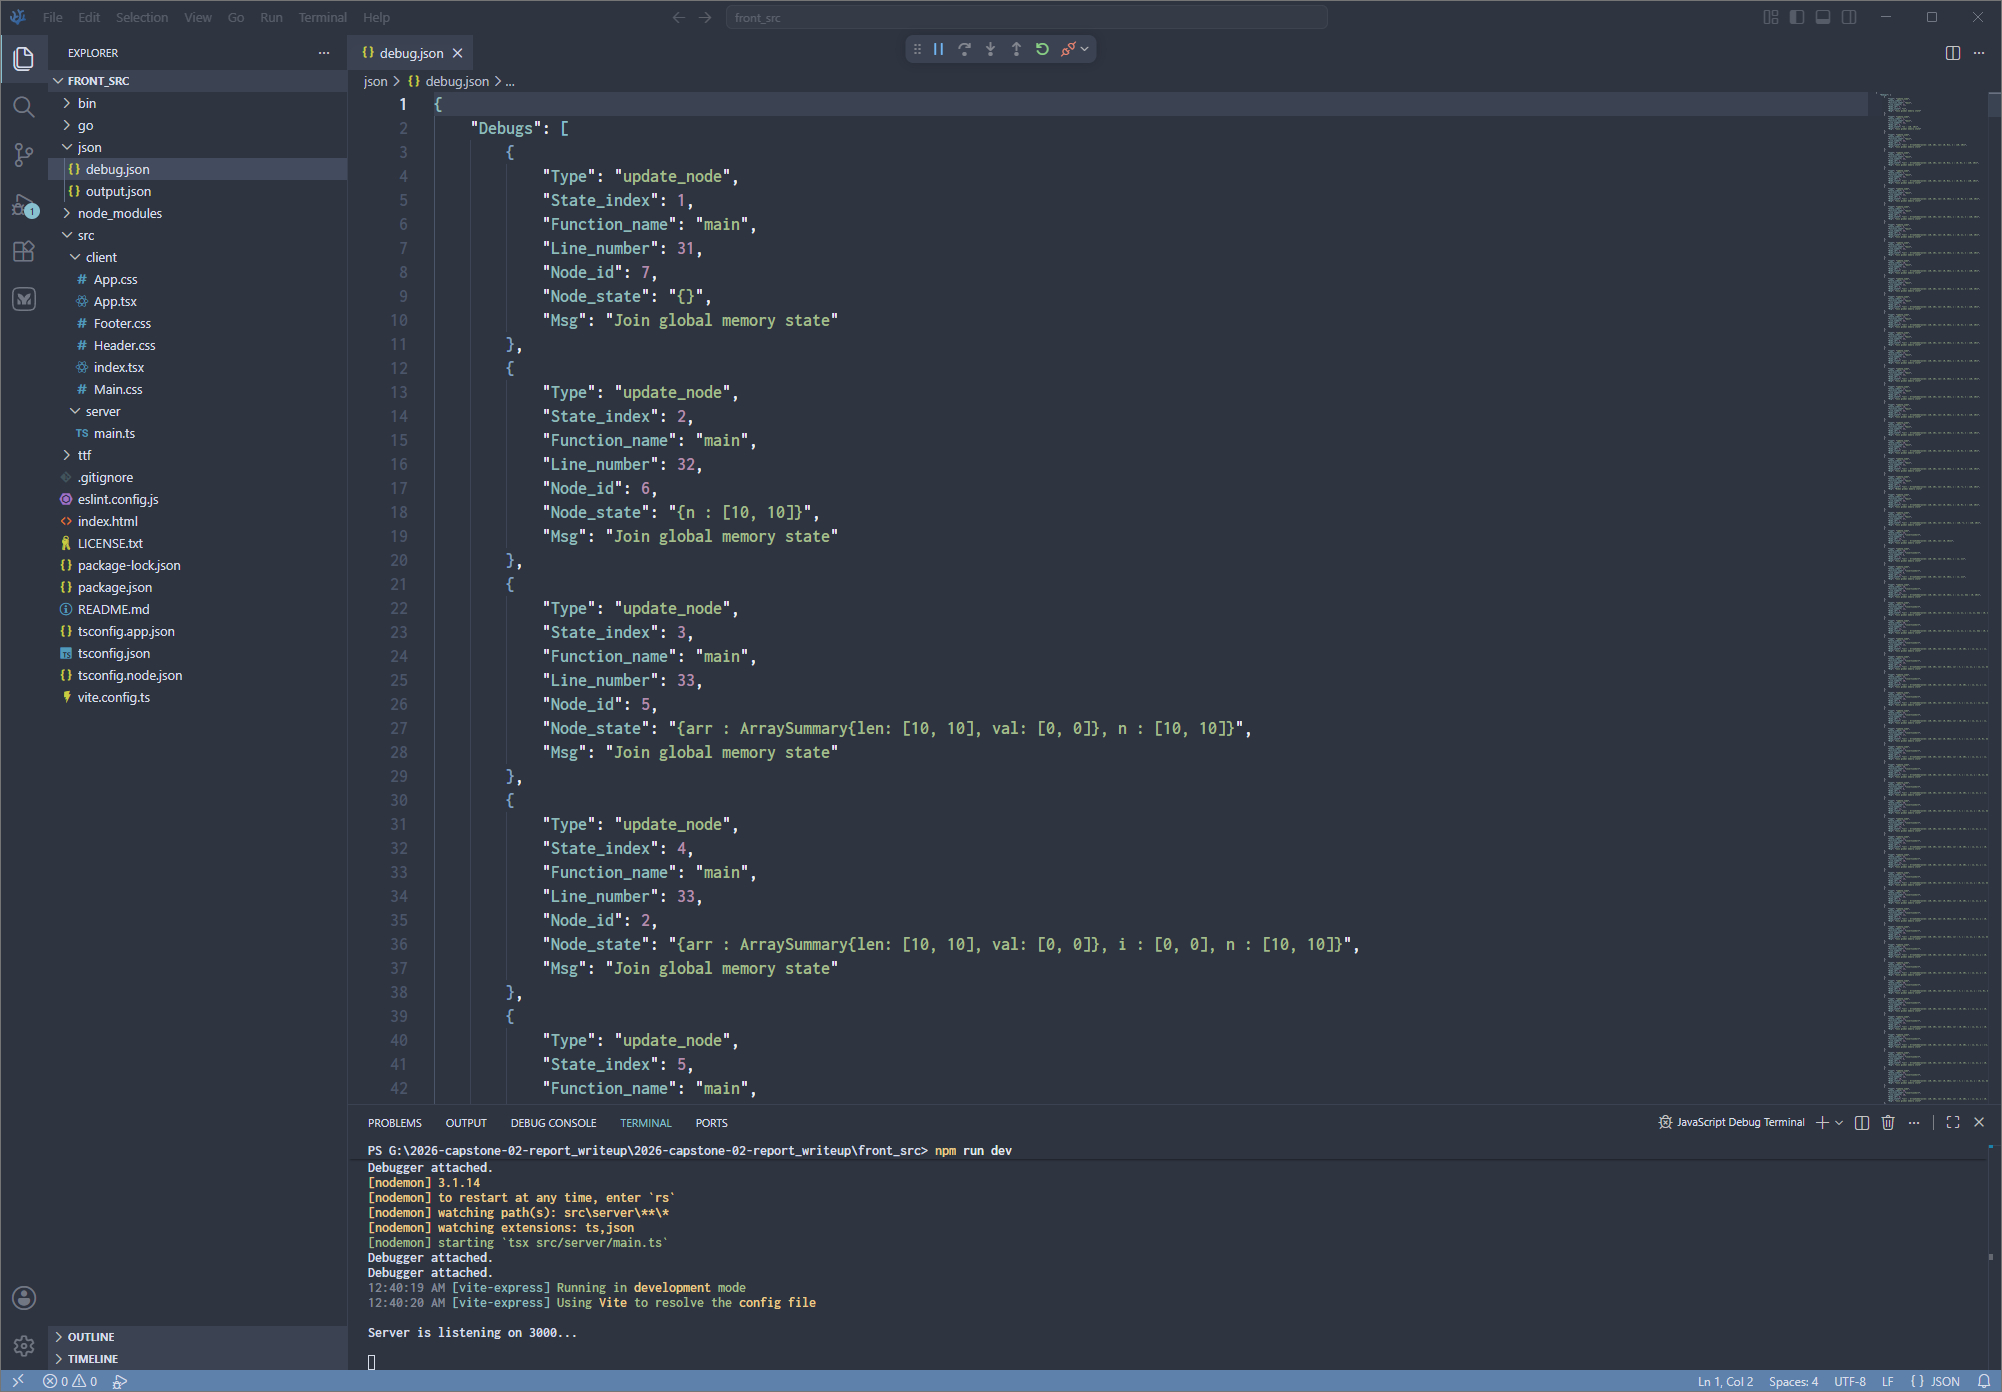
\includegraphics[width=0.8\textwidth]{images/front/04.jpg}
    \caption{2차 그래프 JSON 파일}
\end{figure}

바로 분석 과정을 생성하기 위해, 곧장 ExpressJS로 제작한 서버에 /debug 신호로 넘겨 처리할 준비를 한다.
이 때, \verb|front_src/go/source.go|를 이용하여 다른 플래그로 분석기를 돌리고, 이 과정은 NodeJS 라이브러리 \verb|child_process| 내에 있는 \verb|exec| 함수를 이용한다.
분석기를 돌리면 분석기의 분석 과정이 기록된 JSON 파일이 \verb|front_src/json/debug.json| 생성되고, 이를 JSON 형식으로 클라이언트로 귀속한다.
귀속된 JSON 파일은 2차 MermaidJS 그래프를 제작을 위하여, \verb|Debug_t| 클래스를 만들고 이를 배열로서 저장한다.

\verb|Debug_t| 배열의 귀속된 인스턴스 중, 경고 혹은 오류와 같은 인스턴스는 오른쪽 창에 띄우도록 준비한다.
단, 분석 과정이 기록된 인스턴스들은 따로 다른 배열로 분리시킨 후, 각 변동 과정을 하이라이트한 MermaidJS 소스 코드 배열을 별도로 생성하여 준비한다.
이는, 분석 과정을 조작하여 살펴볼 때, MermaidJS가 유동적으로 변화할 수 없는, 컴파일 되어있는 SVG 형식으로 그래프를 출력하기 때문에,
컴파일을 하기 위한 목적과 함께, 슬라이더 구현도 for-range로 처리할 수 있다는 장점도 겸하고 있어 다음과 같은 방식을 채택하였다.

\begin{figure}[H]
    \centering
    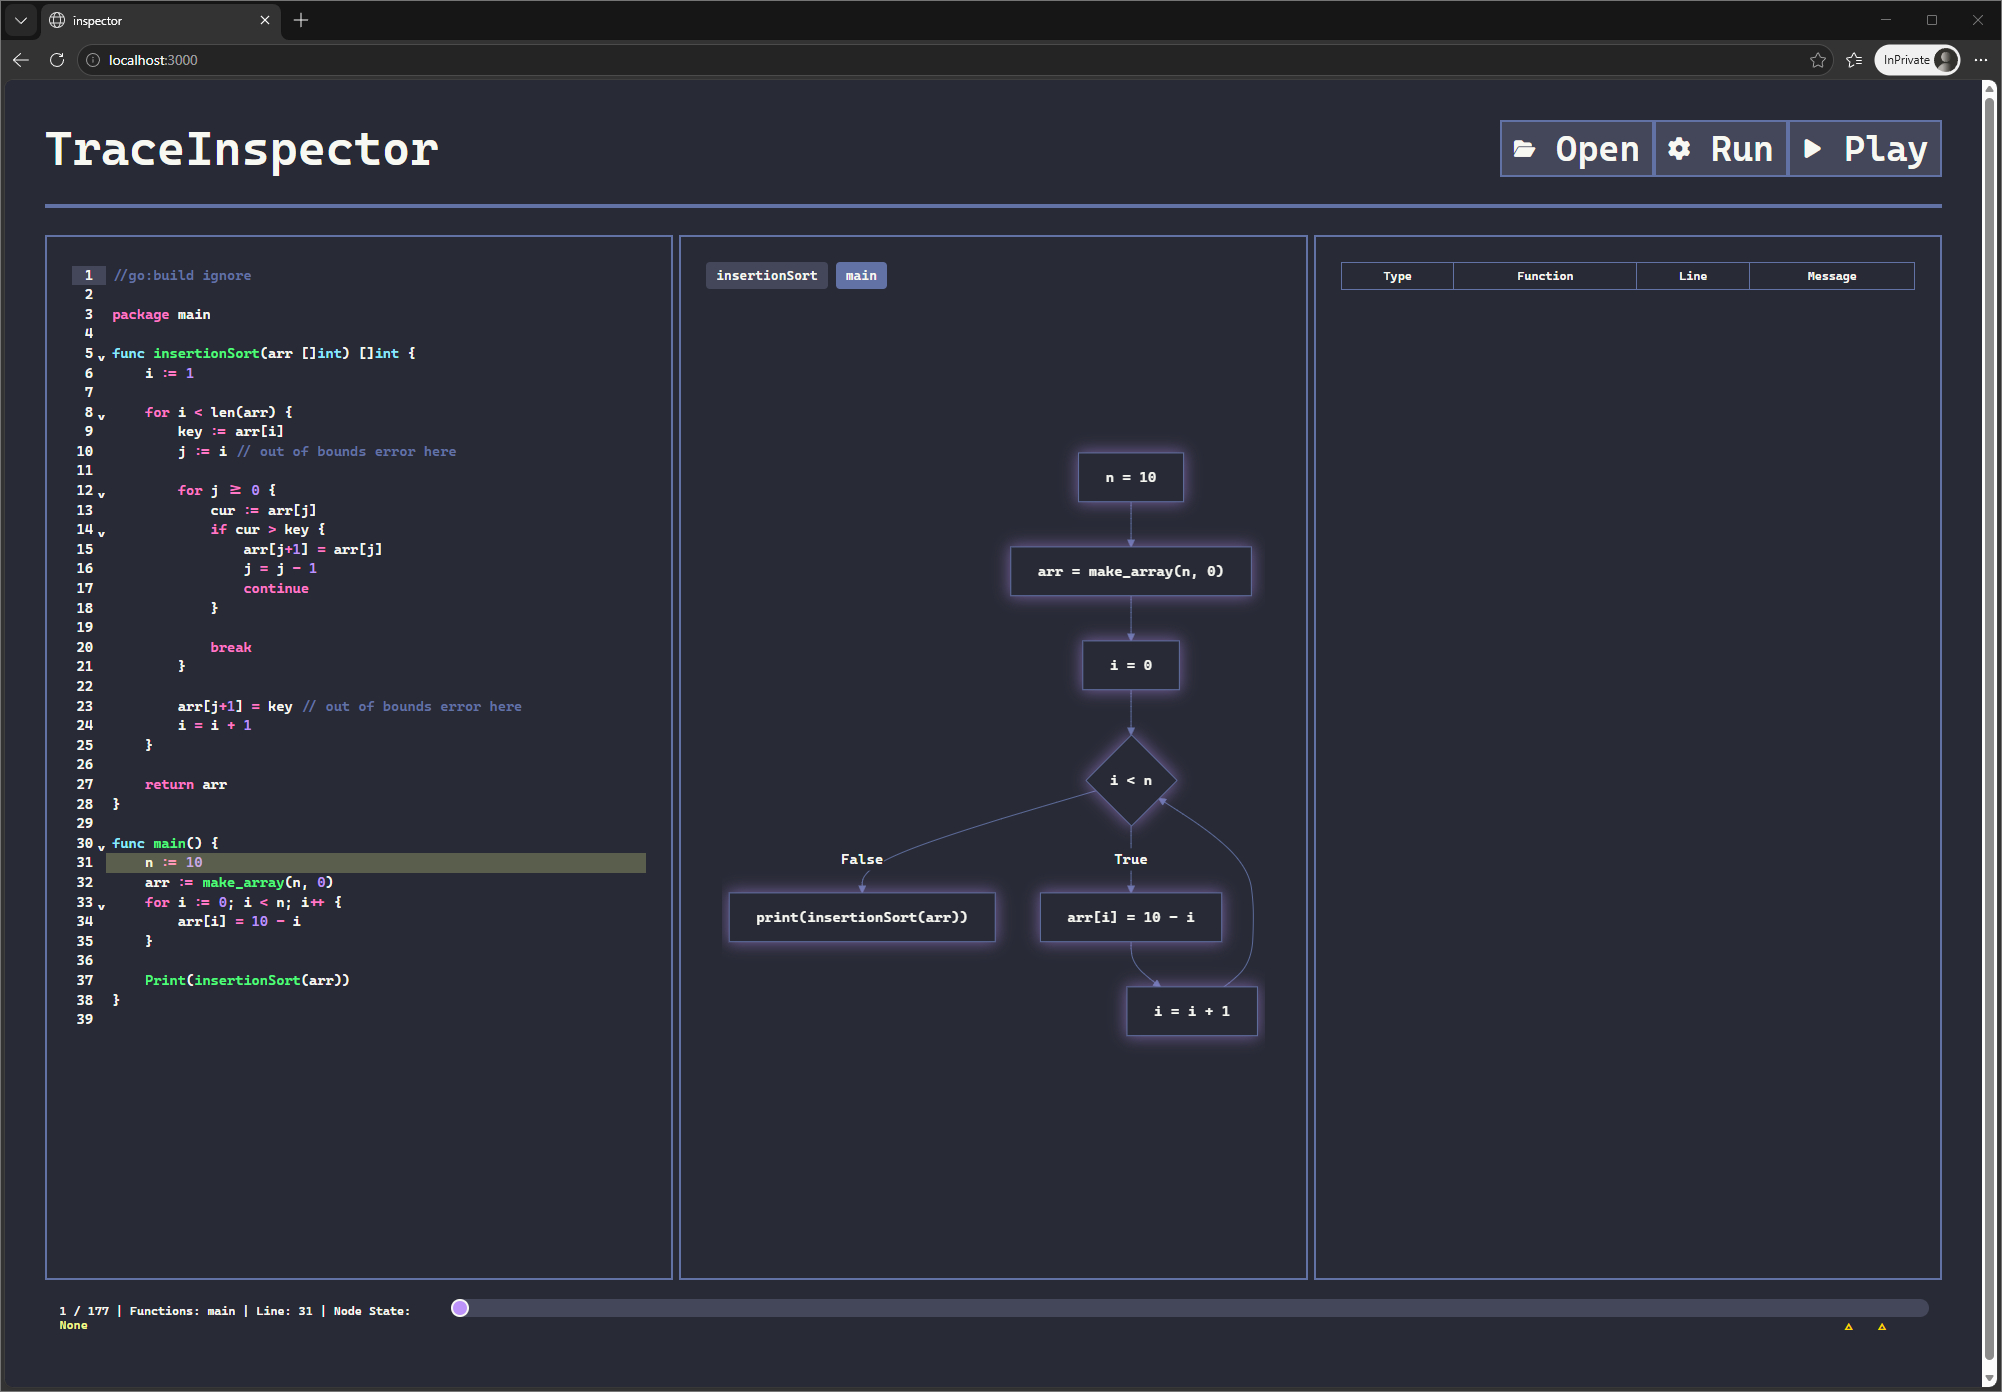
\includegraphics[width=0.8\textwidth]{images/front/05.jpg}
    \caption{Run 이후 UI}
\end{figure}

슬라이더 생성이 완료되면, 각 그래프와 디버그 창을 슬라이더와 연동시키고 Zoom 기능이나 Drag 기능을 위해 부가적인 요소를 초기화한다.
최종적으로, 모든 것들이 연동되어 있는 슬라이더와 2차 그래프를 생성하여 "Run" 연산을 모두 마친다.

이 모든과정은 "Run" 버튼 한번에 클릭으로 이루어지기에, 소스코드가 커지면 그의 비례하여 초기 소요시간이나 메모리 사용량이 증가할 수 있으나,
추가적인 갱신은 이미 완료한 상태이기에, 딜레이의 요소는 슬라이더 조정 간에 생길 수 있는 컴파일 시간이 전부이며, 메모리 사용량은 증가하지 않는다.

\begin{figure}[H]
    \centering
    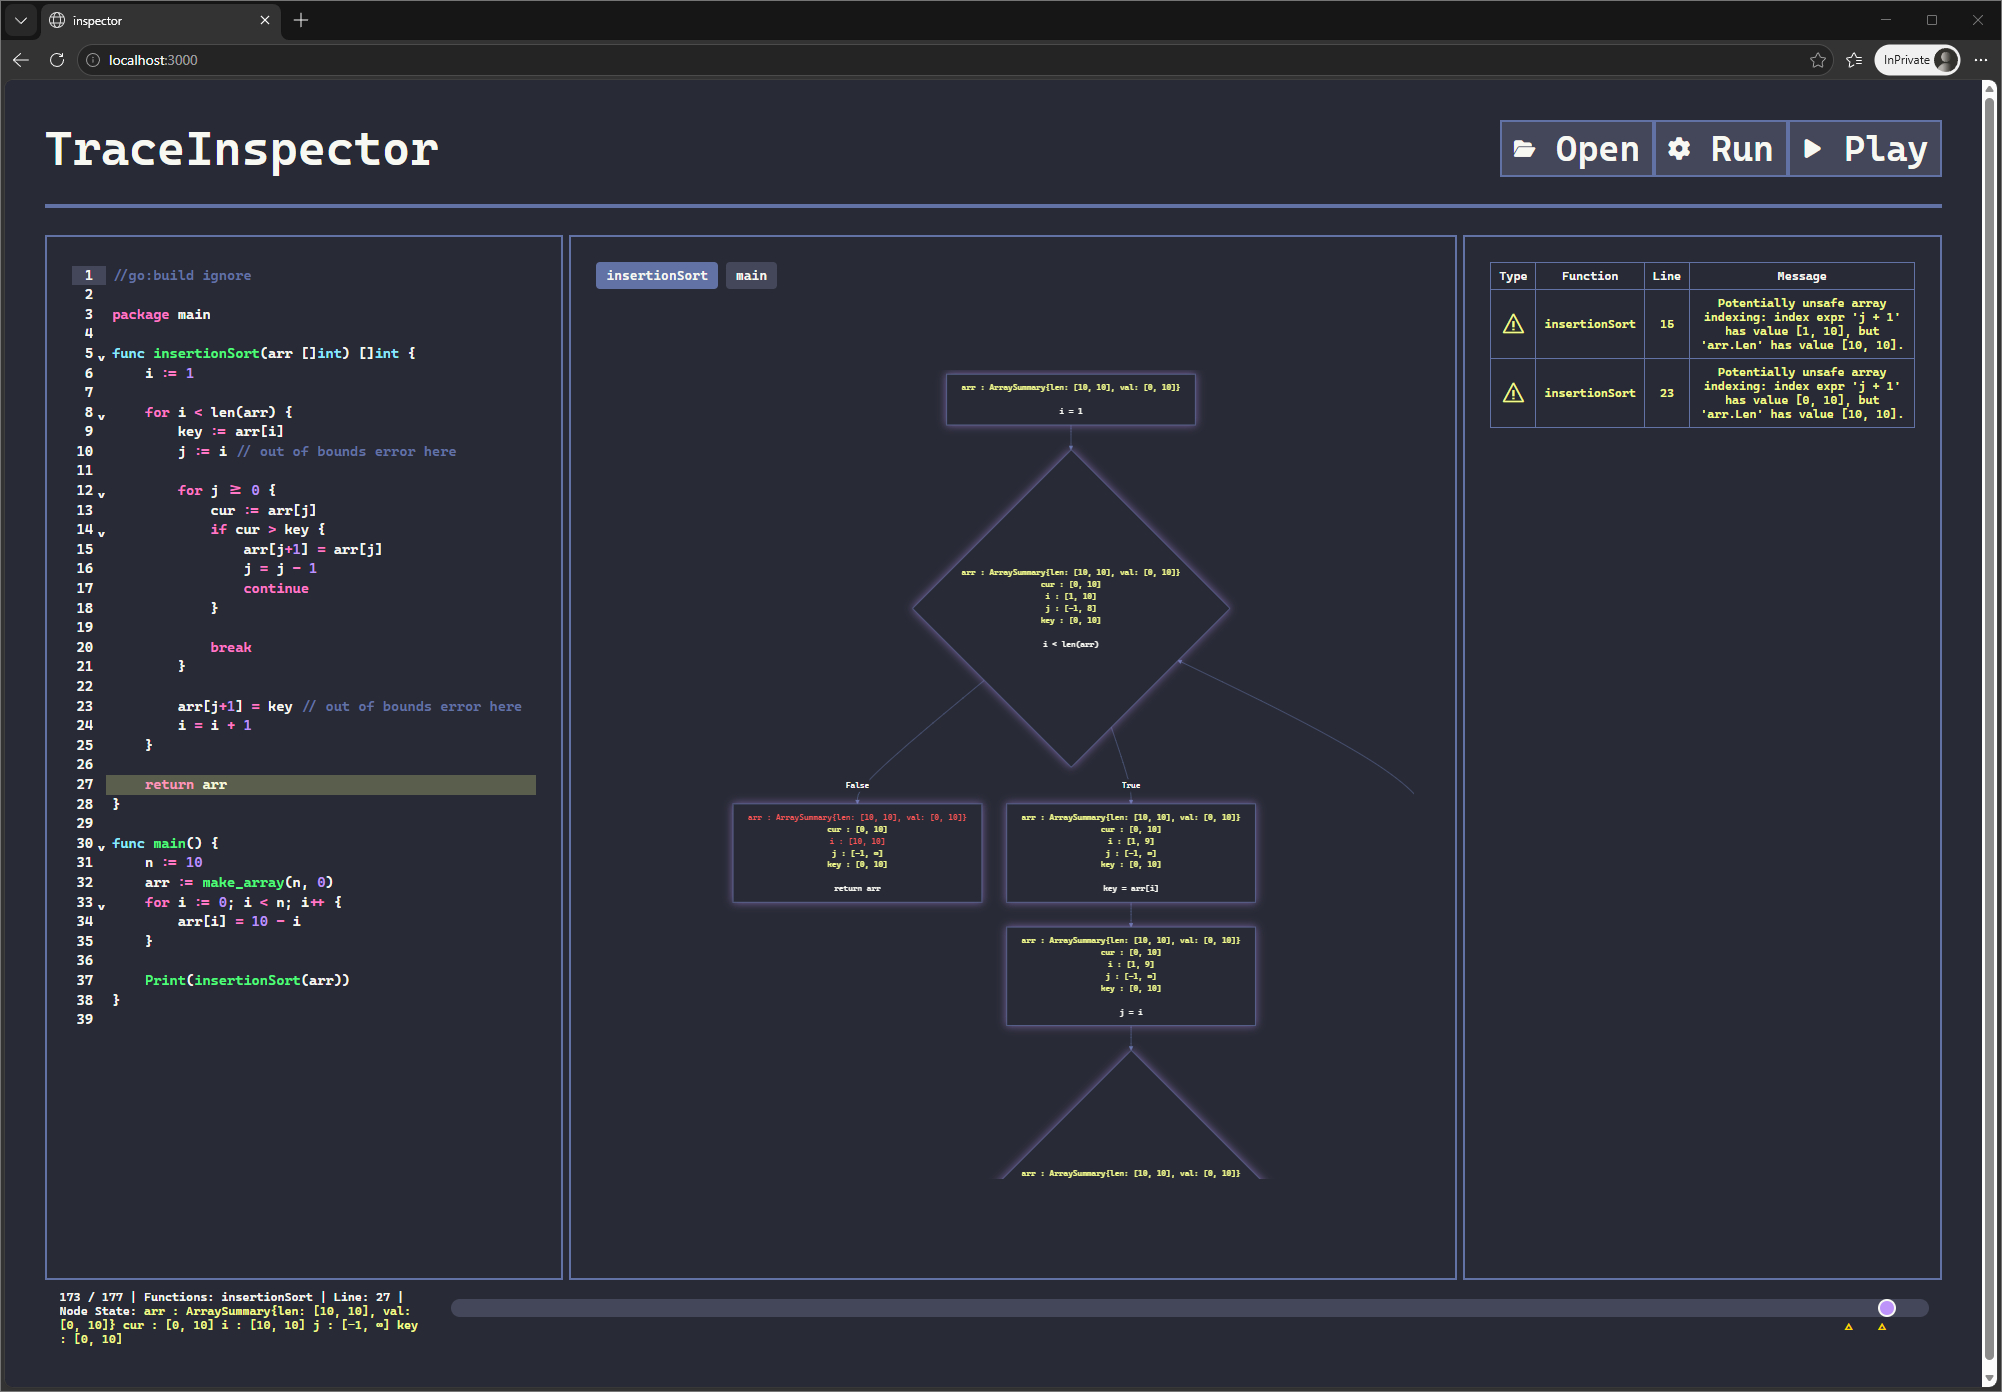
\includegraphics[width=0.8\textwidth]{images/front/06.jpg}
    \caption{실행 중인 UI}
\end{figure}

각 변동사항은 그래프에 빨간색 글씨로 표기되며, 아래 하단에 삼각 점은 경고 및 오류가 발생한 위치를 찍어주는 점이다.
그래프를 조정하여 변동사항을 실시간으로 확인 할 수 있으며, "Play" 버튼을 눌러 자동화 할 수 있다.

\subparagraph{사용요소 상세설명} ~\\

위에서 잠깐 언급했지만, 이 UI를 구성하기 위해 들어간 요소들이 대거 있으며, 이를 간단히 소개하도록 하겠다.

\begin{enumerate}
    \item React + TypeScript + Vite + ExpressJS: 각 요소는 프로그램 작동을 위한 핵심 프레임 요소들이며, 사용자 또한 반드시 각 요소를 설치하여야 동작한다.
    \item Cascadia Mono with Nerd Font: 현 프론트에 사용되었던 글꼴이며, 아이콘 또한 현 글꼴에서 제공되는 아이콘을 사용하였다.
    \item CodeMirror: 가운데 왼쪽에 있는 코드 에디터를 구성하기 위해 사용된 라이브러리다.
    \item Multer: 직접적인 서버 내부 파일 시스템에 입출력을 수행하기 위해 사용된 라이브러리다.
    \item Mermaid: 분석 과정 시각화를 위해 사용된 흐름차트 생성 라이브러리다.
    \item panzoom: 그래프를 확대하거나 드래그 하여 탐색할 수 있도록 사용된 라이브러리다.
    \item Go: 프론트 개발에는 사용되지 않았지만, 동작을 위한 CLI 분석기 제작을 위해 필요한 프로그래밍 언어다.
\end{enumerate}

\subsubsection{시스템 기능 요구사항}

최종적으로 \traceinspector는 다음과 같은 통합 단계를 수행한다:

\begin{enumerate}
    \item 웹 인터페이스를 통해 소스 파일 업로드
    \item \traceinspector 분석기를 소스 파일에 대해 호출
    \item 소스 파일을 \imp로 변환
    \item \imp AST를 CFG로 변환
    \item CFG 위에서 요약 프로그램 상태 고정점 계산
    \item 고정점 상태 위에서 오류 명제 판정
    \item 계산된 요약 상태 시계열 및 오류 정보를 출력
    \item 해당 정보를 웹 인터페이스에 렌더링
    \item 사용자 조작에 따른 인터페이스 갱신
\end{enumerate}


\subsubsection{시스템 비기능(품질) 요구사항} 

\traceinspector 분석기의 절대적인 요구사항은 논리적 건전성 준수이다. 따라서 분석기를 한번에 구현하는 것이 아니라 단계적으로 구현하며 지속적인 코드 리뷰 및 
건정성 검토를 통해 건전성을 추구하고자 하였다.

0단계는 $\mathbb{Z}_{+}$ 정수체계 및 구간도메인 구현 및 검증이었다. 해당 요소들은 분석기의 기반이 되는 요소들이고 산술 연산이 많이 포함된 만큼 구현 후 
코드 리뷰 및 테스팅을 통해 건전성을 확인하엿다.

1단계는 \imp 언어 중 대입 및 식 계산을 구현 목표로 하였다. 반복문과 조건문 등 제어 흐름을 배제하고 오로지 순차적인 명령에 대해서 구현을 하여 구체적 및 요약 의미론의 
commutativity를 검증하고 논리적으로 건전한지 확인하였다.

2단계는 조건문과 배열 타입 지원이다. 조건문의 경우 루프 조건 필터링 함수를 구현해야 하기에 다시금 대수적 연산의 많은 구현을 필요로 해 면밀한 코드 리뷰 및 건정성 검토가 필요했고, 
배열 타입은 요약도메인 선정 및 설계 시의 트레이드오프들을 고려해야 하기에 별도로 상당한 시간을 투자하였다.

3단계는 반복문과 재귀적 함수 호출이다. 두 경우 모드 "무한히 실행되는" 코드가 들어오는 요소들이며, 이에 따라 widening 연산($\triangledown$)과 함수 호출 단위 처리를 구현해야 한다.
특히나 widening 연산의 경우 잘못 구현할 경우 지금까지 쌓아온 논리적 건전성이 무너질 수 있기에 이론적인 배경을 바탕으로 구현 후 테스팅을 많이 수행하였다.

도메인 및 분석기를 설계하는 과정에서 특정 도메인을 하드코딩 하지 않고 인터페이스로 설계하여 향후 새로운 도메인 구현 및 통합이 가능하도록 설계하였다. 이러한 설계는 단순히 확장성을 넘어 
도메인 구현 시 일관적인 구조를 요구하고, 모듈화한 테스팅을 가능케 하여 코드의 품질 및 안전성에 크게 기여를 하였다. 특히나 요약도메인의 타입간 연산을 구별할 수 있게 되어 요약의미론 상에서 
타입 오류가 발생하지 않도록 보장하는 이점을 누릴 수 있게 되었다.

\clearpage
\subsubsection{시스템 구조 및 설계도}

\begin{figure}[H]
    \centering
    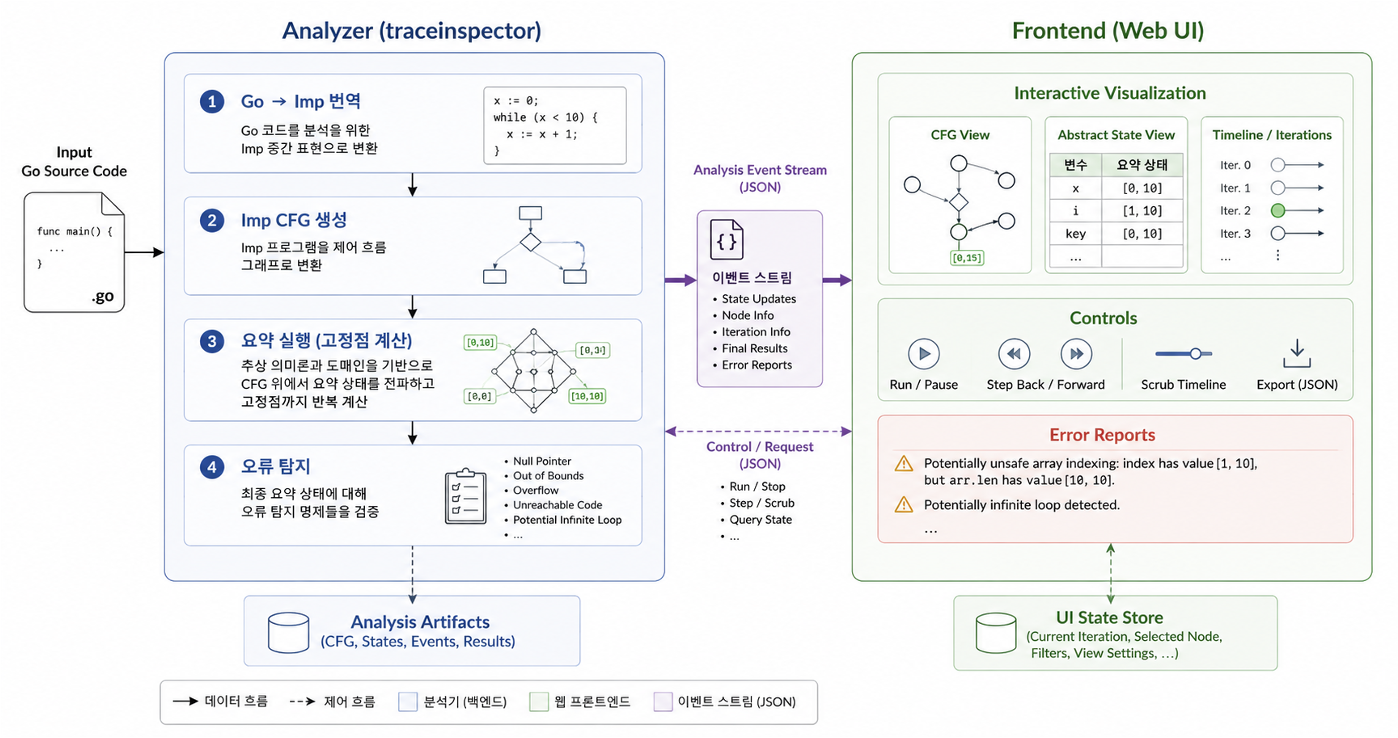
\includegraphics[width=0.99\textwidth]{images/architecture.png}
    \caption{\traceinspector 전체 시스템 구조}
    \label{fig:architecture}
\end{figure}

그림 \ref{fig:architecture}는 \traceinspector 의 전반적인 구조를 나타낸다. \traceinspector 분석기는 입력 Go 프로그램에 대한 요약 프로그램 상태를 계산하여 오류 정보와 함께 JSON 형태로 표준 출력에 출력한다.

\traceinspector 프론트엔드는 사용자로부터 코드를 입력받아 분석기를 호출하여 수행 결과를 시각화하는 웹 인터페이스와 백엔드로 구성되어 있다.

\subsubsection{활용/개발된 기술}

\textsf{TraceInspector} 분석기는 Go 소스 파일 파싱을 위한 \textsf{go/parser}\cite{goparser} 패키지를 활용한다.
이후의 모든 분석 단계는 외부 라이브러리를 활용하지 않고 직접 구현되었지만 상술했듯이 요약해석 이론 자체는 잘 알려진 정적 분석 기법이다.

\textsf{TraceInspector} 분석기 UI는 다음과 같은 요소들을 사용한다.

1. React + TypeScript + Vite + ExpressJS: 각 요소는 프로그램 작동을 위한 핵심 프레임 요소들이며, 사용자 또한 반드시 각 요소를 설치하여야 동작한다.
2. Cascadia Mono with Nerd Font: 현 프론트에 사용되었던 글꼴이며, 아이콘 또한 현 글꼴에서 제공되는 아이콘을 사용하였다.
3. CodeMirror: 가운데 왼쪽에 있는 코드 에디터를 구성하기 위해 사용된 라이브러리다.
4. Multer: 직접적인 서버 내부 파일 시스템에 입출력을 수행하기 위해 사용된 라이브러리다.
5. Mermaid: 분석 과정 시각화를 위해 사용된 흐름차트 생성 라이브러리다.
6. panzoom: 그래프를 확대하거나 드래그 하여 탐색할 수 있도록 사용된 라이브러리다.
7. Go: 프론트 개발에는 사용되지 않았지만, 동작을 위한 CLI 분석기 제작을 위해 필요한 프로그래밍 언어다.

\subsubsection{현실적 제한 요소 및 그 해결 방안}

\traceinspector 분석기는 본질적으로 입력 언어인 Go의 일부분에 대해서만 분석을 수행할 수 있다. 우선적으로 포인터 자료형에 대한 분석을 지원하지 않는다. 
요약 실행의미론과 요약 프로그램 상태에서는 포인터나 주소 등의 위치와 참조의 개념 없이 오직 단일 값으로만 간주하였고, 지금의 요약 프로그램 상태는 포인터 자료형에 대한 추론을 할 수 없다.
포인터 자료형에 대한 분석은 abstract heap라는, $\mathsf{AbstractVarMemMap} : \mathbb{V} \rightarrow \mathsf{AbstractValue}$가 아닌 
주소 $\mathbb{A}$를 값으로 대응하는 $\mathsf{AbstractHeap} : \mathbb{A} \rightarrow \mathsf{AbstractValue}$를 구현하여 논해야 한다.

또한 추론 가능한 식의 구체적 형태에 대한 제한이 존재한다. \traceinspector는 $\pm x \pm y \odot C$ 형태의 대수식에 대한 논리적 추론 및 제약 역산을 수행할 수 있다.
하지만 구체적인 동작 형태는 $x, y, C$에 대한 요약도메인 값을 산출하기에, 실제 $x, y, C$간의 논리적 관계에 대해 알 수 없다.
\begin{lstlisting}
while (x < len(arr)) {
    Print(arr[x - 1])
}
\end{lstlisting}
와 같은 코드가 주어졌을 때, 각 변수의 값을 계산하지 않고 \verb|x|는 항상 \verb|len(arr)|의 길이보다 작다는 \textit{관계형} 정보를 추론할 수 있다.
이러한 관계형 정보를 표현하기 위해선 Octagon\cite{mine2006}, Convex Polyhedra등의 관계형 도메인과 여러 도메인 사이의 정보를 보안할 수 있는 reduced produc 도메인\cite{cousot2011}을 구현하고 논리적 조건식에 대한 정보를 구하는 형태의 분석기가 필요하다.
따라서 \traceinspector는 관계형 정보에 대한 추론 능력에 대한 제한사항이 존재한다.

이러한 특성은 구현된 요약도메인의 정확도에 구애받기에, 향후 보다 정확하고 다양한 정보를 표현할 수 있는 요약도메인을 구현하고, \traceinspector 분석기와 통합하는 작업이 필요할 것이다.

마지막으로 현재 구현된 분석기는 입력 언어가 단일 Go파일로 제한되어 있다. 설계 자체는 타 언어 $\rightarrow$ \imp로의 번역기로 확장 가능하지만, 단일 파일에 대한
분석이라는 한계는 여전히 존재한다. 이에 따라 입력 언어형태에 맞는 전처리기를 구현하여 모듈 단위의 분석을 지원할 수 있도록 개선이 필요하다.

재귀적인 함수 역시 분석의 정확도를 저하시킨다. 현재 분석기는 함수 단위로 분석을 수행하기에 새로운 함수 호출에 진입한 경우 함수의 인지값으로부터 함수 내부 상태에 대한 계산을 새롭게 수행해야 한다.
즉 필요한 시공간적 자원은 호출 스택의 깊이에 비례해서 증가하게 된다. 더욱 더 문제가 되는 점은 이러한 재귀적 호출의 경우 호출자의 프로그램 상태와 인자에 대한 논리적인 성질을 추론하지 않는다는 점이다.
재귀 함수의 경우 total recursion 성질을 만족하면 재귀가 언젠가는 종료한다는 것이 알려져 있다. 즉 호출자의 프로그램 상태의 값들에 대해 인자들이 단조 감소하는 것이 보여진다면(decreasing argument),
재귀 함수의 호출 체인이 언젠가는 종료할 것이라는 고수준의 추론이 가능하다. 이처럼 함수 단위가 아닌 호출자와 피호출자 간의 정보에 대해 추론하는 intra-procedural 분석을 구현한다면 보다 정확한 추론이 가능할 것이다.

결론적으로 정확하고 신뢰할 수 있는 분석기를 만드는 문제는 
\begin{enumerate}
    \item 분석 대상 언어의 기능 중 어느 부분집합만을 구현할 것인지
    \item 요약 도메인 선정 및 구현 시 시공간적 비용과 정확도의 트레이드오프를 어떻게 조율할 것인지
    \item 얼만큼의 허위 경보를 용납할 것인지
\end{enumerate}
과 같은 디자인 결정에 크게 영향받는다. 특히 이러한 문제들은 최적의 정해가 주어진 것이 아니라 트레이드오프 관계에 해당되는 만큼 분석기가 사용되고자 하는 영역의 특성과 도메인 지식을 활용하여 
설계되어야 한다. 이러한 문제는 실제 분석기 개발자들도 많은 시간과 연구를 통해 지속적으로 개선하고 있는 영역이다. 
따라서 이번 프로젝트를 통해 정적 분석 이론은 구현 가능했지만, 실제로 쓸만한 분석기를 만드는 것은 이론을 넘어 경험과 노하우가 압도적으로 중요하다는 점을 깨닫게 되었다.

\subsubsection{결과물 목록} \label{artifact}

\traceinspector 의 소스는 루트 경로 내에 \verb|traceinspector| 와 \verb|front_src| 로 크게 나누어져 있다.

\verb|traceinspector| 경로는 분석기 구현체를 담고 있으며, 다음과 같은 하위 경로로 세분화되어 있다.

\verb|algebra| 경로에는 분석기에서 활용되는 확장된 정수체계 및 대수적 논리식 조작 체계를 수록하고 있다:
\begin{itemize}
    \item \verb|extended_integers.go|는 무한대로 확장한 정수체계 $\mathbb{Z}_{\infty}$를 나타내는 \verb|ExtInt| 구조체와 관련 연산들을 구현한다.
    \item \verb|simple_prop.go|는 $\pm x \pm y \odot C$ 형태의 대수식을 나타내는 \verb|SimpleProp| 구조체와 수식 조작, 그리고 $\mathsf{SimpleProp} \Leftrightarrow \mathsf{Imp}$식(expression)간의 변환을 구현한다.
    \item \verb|arith_normalizer.go|는 $a_1 x_1 + a_2 x_2 +  ... a_n x_n + C $ 형태의 다항식을 나타내는 \verb|Polynomial| 구조체와 수식 조작, 그리고 마찬가지로 \imp 식간의 변환을 구현한다.
\end{itemize}

\verb|cmd| 경로에는 분석기의 실행파일 생성을 위한 진입점 및 명령줄 인터페이스를 구현한 \verb|main.go|를 수록하고 있다.

\verb|domain| 경로에는 \traceinspector 분석기의 요약 도메인 추상 인터페이스 및 정수 구간과 Bool 요약도메인, 그리고 filter 함수 $\mathcal{F}_{B}$ 인터페이스 및 구현을 수록하고 있다:
\begin{itemize}
    \item \verb|domain.go|는 요약도메인의 추상 인터페이스 \verb|AbstractDomain|와 정수 요약도메인의 추상 인터페이스 \verb|IntegerDomain|를 구현한다.
    \item \verb|array_top_domain.go|는 모든 배열을 $\top$로 요약하는 약식 배열 요약도메인을 구현한다.
    \item \verb|bool_domain.go|는 Bool 요약도메인 및 관련 연산을 구현한다.
    \item \verb|interval.go|는 구간 요약도메인 및 관련 연산을 구현한다.
    \item \verb|filter_query.go|는 filter 함수 구현을 위한 \verb|FilterQuery| 구조체 및 논리식의 형태를 정의한다.
    \item \verb|filter.go|는 \verb|SimpleProp|로부터 \verb|FilterQuery|를 구할 수 있는 변환 함수 및 대수적 조작 함수들을 구현한다.
\end{itemize}

\verb|imp| 경로에는 \imp의 정의와 Go $\rightarrow$ \imp 번역기, 그리고 \imp 의 구체적 실행의미론을 구현한 인터프리터를 수록하고 있다.
\begin{itemize}
    \item \verb|imp.go|는 \imp의 문법과 타입 정의, AST 구조체들을 구현한다.
    \item \verb|interpreter.go|는 \imp의 구체적 실행의미론을 구현한, \imp 프로그램을 실행하는 인터프리터를 구현한다.
    \item \verb|go2imp.go|는 Go AST를 \imp AST로 번역하는 번역기를 구현한다.
\end{itemize}

탑레벨 \verb|traceinspector| 경로에는 다음과 같은 중요 소스 파일들이 존재한다:
\begin{itemize}
    \item \verb|abstract_mem.go|는 $\mathsf{AbstractValue}, \mathsf{AbstractVarMemMap}, \mathsf{AbstractNodeMemMap}$, 그리고 함수별 요약상태 저장용 \verb|AbstractFunctionMem| 을 구현한다.
    \item \verb|analyzer.go|는 고정점 계산 및 \imp 의 요약 실행의미론을 구현한 \verb|AbstractAnalyzer| 구조체를 구현한다.
    \item \verb|array_domain.go|는 배열 타입에 대한 요약도메인의 추상 인터페이스 \verb|ArrayDomain|를 구현한다.
    \item \verb|array_summary_domain.go|는 배열 원소 축약 요약도메인을 구현한다.
    \item \verb|cfgdefs.go|는 CFG 노드 및 간선들과 관련된 정의를 구현한다.
    \item \verb|create_cfg.go|는 \imp AST를 CFG로 번역하는 알고리즘을 구현한다.
\end{itemize}

\verb|front_src| 경로는 분석기 UI를 담고 있으며, 다음과 같은 하위 경로로 세분화되어 있다.

\verb|bin| 경로에는 UI에서 활용되는 CLI 분석기 바이너리가 생성되어 있어야 한다:
\begin{itemize}
    \item \verb|traceinspector.o|는 UNIX 계열에서 돌릴 수 있는 build.sh 스크립트를 실행 하였을 때, 생성되는 CLI 분석기 바이너리 이름이다.
    \item \verb|traceinspector.exe|는 Windows 계열에서 돌릴 수 있는 build.bat 스크립트를 실행 하였을 때, 생성되는 CLI 분석기 바이너리 이름이다.
\end{itemize}

\verb|json| 경로에는 CLI 분석기 바이너리가 서버에서 작동 시 만들어 주는 JSON 파일들이 생성되어 있어야 한다:
\begin{itemize}
    \item \verb|output.json|은 1차 MermaidJS 흐름 차트 생성을 위한 그래프 노드 및 엣지 정보가 출력된다.
    \item \verb|debug.json|은 2차 MermaidJS 흐름 차트 생성을 위한 분석 과정 정보가 출력된다.
\end{itemize}

\verb|ttf| 경로에는 분석기 UI가 사용하는 글꼴들이 존재한다:
\begin{itemize}
    \item \verb|CaskaydiaCoveNerdFontMono-*.ttf|는 유니코드 문자셋을 변형하여 많은 아이콘을 추가한 "Nerd Font"와 "Cascadia Mono"를 합친 글꼴이다.
\end{itemize}

\verb|src| 경로에는 분석기 UI 제작에 사용된 소스코드를 담고 있으며, 다음과 같은 하위 경로로 세분화되어 있다.

\verb|client| 경로에는 ReactJS 클라이언트 제작을 위해 사용한 소스 파일이 존재한다:
\begin{itemize}
    \item \verb|App.css|는 전체 UI에 적용되는 기본 스타일을 정의한다.
    \item \verb|App.tsx|는 실질적인 UI 제작에 사용된 모든 함수 및 기능을 구현한다.
    \item \verb|Footer.css|는 하단 UI 요소들에 적용되는 스타일을 정의한다.
    \item \verb|Header.css|는 상단 UI 요소들에 적용되는 스타일을 정의한다.
    \item \verb|index.tsx|는 App.tsx 파일과 index.html 파일을 연결해주는 파일이다.
    \item \verb|Main.css|는 중간 UI 요소들에 적용되는 스타일을 정의한다.
\end{itemize}

\verb|server| 경로에는 ExpressJS 서버 제작을 위해 사용한 소스 파일이 존재한다:
\begin{itemize}
    \item \verb|main.ts|는 클라이언트와 상호작용하는 모든 호출을 처리하는 함수 및 기능을 구현한다.
\end{itemize}

탑레벨 \verb|front_src| 경로에는 다음과 같은 중요 소스 파일들이 존재한다:
\begin{itemize}
    \item \verb|index.html|는 최상단 HTML 문서이다.
    \item \verb|package.json|는 분석기 UI 제작에 사용되는 npm 라이브러리를 기술한 파일들이다.
    \item \verb|eslint.config.js|는 JavaScript 정적분석기 설정을 정의하는 파일이다.
    \item \verb|vite.config.ts|는 Vite 핸들러가 사용하는 설정을 정의하는 파일이다.
    \item \verb|tsconfig*|는 TypeScript 컴파일러가 사용하는 설정을 정의하는 파일들이다.
\end{itemize}

\subsection{기대효과 및 활용방안}

본 분석기는 기존의 상용화된 분석기처럼 효율적이고 정확성 관점에서 경쟁하고자 구현한 것이 아니라. 오히려 반대로 효율성을 희생하고 그 동작 과정을 노출시켜 관찰 가능한 정적 분석기를 구현하고자 하였다.

정적 분석을 사용해본 경험은 있지만 구체적인 원리에 대해 잘 알지 못하는 소프트웨어 개발자들에게는 정적 분석 기술이 어떤 방식으로 동작하고, 단순히 한번에 결과가 계산되는 것이 아닌 반복적인 알고리즘임을 
전달하기를 기대한다. 컴퓨터공학을 전공했다면 알고리즘 강의 때 복잡해보이는 알고리즘도 단계적으로 절차에 따른 연산을 수행한다는 점으로 분해해서 볼 수 있듯이 정적 분석도 마찬가지임을 알리고자 한다. 
또한 프로그램 분석이라는 기술과 이론을 소개하면서 올바른 코드란 무엇인지, 그리고 프로그램에 대해 어떻게 논증할 수 있는지에 대해 생각해볼 기회를 제공하고자 한다.

정적 분석 혹은 요약해석을 공부했거나 공부하고자 하는 경우 보다 구체적인 도움을 제공할 수 있을 것으로 계산된다. 대부분의 이론 교과서는 \textit{프로그램의 요약 메모리 상태에 대해 요약 의미론이 정의한 전이 단계를 반복적으로 수행하며 고정점을 계산한다} 라는 형태로 
분석 알고리즘을 소개한다. 물론 자명한 결과지만 간단한 예제를 넘어 실제로 어떻게 동작하는지에 대한 직관은 파악하기 어렵고 와닿는 설명이라고 보기는 어렵다. 고정점 계산이라는 개념을 상호작용 가능한 시계열 정보로 나열하여 직접 변화를 관찰할 수 있게 제공하고, 구체적인 그래프 위에서 
의미론의 전이 과정과 상태 갱신 과정을 파악할 수 있음으로써 이론을 직관적으로 이해할 수 있도록 도움을 주는 보조 도구로써의 역할을 수행할 수 있을것이라 기대된다.

\section{자기평가}

\traceinspector 분석기를 구현하게 되면서, 요약해석 알고리즘이 실제로 어떻게 고정점을 계산하고, 실시간으로 어떻게 프로그램 상태를 추정하는지 그 과정을 관찰할 수 있어서 매우 흥미로웠다.
이 프로젝트를 진행하기 전부터 요약해석 이론에 대해서는 알고 있었지만 단순히 이론적으로 "반복을 통해 고정점을 계산한다"는 사실을 기호로써만 터득했지 실제로 어떤 형태로 그 과정이 동작하는지, 
그리고 왜 항상 고정점에 도달할 수 있을지에 대해서는 크게 관심을 가지지 않았다.

하지만 분석기를 구현하고 처음으로 프론트엔드와 연결하여 시각화한 결과를 보니 정말로 "이론이 살아 움직이는" 직접적인 결과를 볼 수 있어서 아름답게 느껴졌다. 특히나 단순하게 요약해석 분석기를 구현하고 끝나는 것이 아니라 
시각화 인터페이스와 연결하여 보여주는 만큼, 두 구성 요소간의 통합을 설계하고 시계열 형태로 분석 결과를 생성하는 분석기를 만들었기에 좋은 경험이었다.

마지막으로 프로그램이 단순히 텍스트에 불과한게 아닌 분석과 논증의 대상으로 인식하게 되었고, 프로그램 분석과 언어론이 논리학과 수학의 근원적인 문제들과 직접적인 연관성을 가지고 있음을 체감하게 되었다.
프로그래밍이 대중화되고 "소프트웨어"라는 결과물을 만드는 것에 집중을 하다보니 프로그래밍이 무엇인지, 그리고 프로그램 자체가 무엇인지에 대해서 깊게 생각해볼 기회는 많지 않았다.
따라서 이번 프로젝트를 통해 "프로그램, 실행, 오류" 등의 의미에 대해 심도있게 탐구해볼 수 있어 만들어낸 산출물 이상의 가치가 있는 시간이었다고 스스로 생각한다.

프론트엔드 담당의 경우 초반에 많이 접하지 못한 부분을 도전하면서 시간 조절을 못하여 프론트 개발이 많이 더딘 점이 있었다. 
또한 분석기의 출력을 프론트와 연동하는 과정과 UI 스타일을 짜는것도, 디자인 부분에서의 창의력을 발휘해야 하기에 많이 우왕자왕하는 모습을 보였다고 생각한다. 
하지만 이러한 딜레이와 문제점을 해결하기 위해 여러 자료를 찾아 생각도 못했던 영감을 얻기도 하였다. 
특히 여러 요소들을 다방면으로 연동해야 하기에 문제발생이 잦는 문제도 많아 이 점을 보고받기 용이하게 Github Issue를 적극적으로 사용해 보았으며, 여러 환경에서 연동하여도 문제가 없도록 각각의 가상머신을 구축하여 테스트를 진행하였다. 
아이콘과 같은 Asset 사용도 일반 이미지 대신의 아이콘을 포함한 글꼴 사용해 관리가 수월해지게 개선하였으며 디자인 테마도 다양하게 찾아보고 적용해 심플함을 살리며 너무 단순하게 보이지는 않도록 많은 노력을 하였다. 
이 과정에서 많은 문제해결 능력과 경험을 쌓게 되었다고 생각한다.

\section{참고 문헌}
\bibliographystyle{plain}
\bibliography{ref}

\section{부록}
\subsection{사용자 메뉴얼}

\traceinspector 웹 인터페이스에서 분석 대상 Go 소스 파일을 Open을 통해 분석을 요청한다. 이후 인터페이스는 업로드한 소스코드와 이에 대응되는 CFG, 그리고 오류 발생 여부를 표시한다.

사용자는 이후 하단의 재생 바를 드래그하여 각 분석 단계별 요약 프로그램 상태를 CFG상에서 관측할 수 있으며, 좌/우 방향키를 이용하여 한 단계별 이동을 할 수 있다.

CFG는 각 함수 단위로 생성되며, 함수별 명령문과, 명령문이 실행될 프로그램 상태를 표시한다. 현 분석 단계에서 갱신된 프로그램 상태를 붉은색으로 음영 처리되어 변화를 직접 확인할 수 있다.

CFG 탐색 창은 드래그와 스크롤을 통해 이동 및 확대가 가능하며, 더블클릭을 통해 상태를 초기화할 수 있다.

마지막으로 재상 바 하단의 노란색 화살표는 오류 상태가 최초로 탐지된 분석 단계를 나타낸다. 화살표를 클릭하면 해당 분석 상태로 이동하고, 오류 정보와 더불어 어떤 명령의 어떤 변수 상태에서 오류가 발생하게 되었는지 관찰 가능하다.

\subsection{운영자 메뉴얼}

\traceinspector 분석기를 127.0.0.1:3000 에서 활성화하기 위해, 다음과 같은 작업이 있어야 한다.

\begin{enumerate}
    \item Go와 NodeJS를 설치한다.
    \item 운영체제에 맞게 \verb|build.sh| 혹은 \verb|build.bat|을 실행한다.
    \item \verb|front_src| 폴더가 경로로 되게 끔 터미널을 실행한다.
    \item \verb|node_modules| 또는 \verb|package-lock.json|가 존재한다면 즉시 삭제한다. (단, 초기 설정에만 해당한다.)
    \item \verb|npm install| 명령을 실행하여, 환경 설치 및 라이브러리를 다운받는다.
    \item \verb|npm run dev| 명령을 실행하여, 서버를 개설한다.
\end{enumerate}

\subsection{배포 가이드}
\subsection{\textsf{Imp} 형식 의미론} \label{imp_semantics}
\newcommand{\evale}{\Downarrow}
\newcommand{\evals}{\Downarrow}
\newcommand{\Normal}{\mathsf{normal}}
\newcommand{\Break}{\mathsf{break}}
\newcommand{\Continue}{\mathsf{continue}}
\newcommand{\Return}{\mathsf{return}}

해당 부록은 \imp에 대한 big-step operational semantics의 일부를 수록한다. 

프로그램 상태 $\sigma : \mathbb{V} \rightarrow \mathbb{v}$는 각 변수를 값으로 대응시킨다.

식(expression)의 경우 프로그램 상태 $\sigma$에서 식 $e$를 실행했을 때 값 $v$로 계산됨을 $\sigma \vdash e \Downarrow v$로 표현한다.

함수의 경우 각 함수 이름을 인자명들과 함수 몸통 명령문의 쌍으로 대응시키는 전역 함수 대응 $F : FunName \rightarrow (\mathbb{V}^*, S)$로 표현된다.

\begin{mathpar}

\inferrule*[right=E-Var]
{}
{\sigma \vdash x \Downarrow \sigma(x)}

\inferrule*[right=E-Int]
{}
{\sigma \vdash n \Downarrow n}

\inferrule*[right=E-Bool]
{}
{\sigma \vdash b \Downarrow b}

\inferrule*[right=E-String]
{}
{\sigma \vdash s \Downarrow s}

\inferrule*[right=E-Add]
{
\sigma \vdash e_1 \Downarrow n_1 \\
\sigma \vdash e_2 \Downarrow n_2
}
{
\sigma \vdash e_1 + e_2 \Downarrow n_1+n_2
}

\inferrule*[right=E-Sub]
{
\sigma \vdash e_1 \Downarrow n_1 \\
\sigma \vdash e_2 \Downarrow n_2
}
{
\sigma \vdash e_1 - e_2 \Downarrow n_1-n_2
}

\inferrule*[right=E-Mul]
{
\sigma \vdash e_1 \Downarrow n_1 \\
\sigma \vdash e_2 \Downarrow n_2
}
{
\sigma \vdash e_1 * e_2 \Downarrow n_1n_2
}

\inferrule*[right=E-Div]
{
\sigma \vdash e_1 \Downarrow n_1 \\
\sigma \vdash e_2 \Downarrow n_2
}
{
\sigma \vdash e_1 / e_2 \Downarrow n_1/n_2
}

\inferrule*[right=E-Neg]
{
\sigma \vdash e \Downarrow n
}
{
\sigma \vdash -e \Downarrow -n
}

\inferrule*[right=E-Eq]
{
\sigma \vdash e_1 \Downarrow v_1 \\
\sigma \vdash e_2 \Downarrow v_2
}
{
\sigma \vdash e_1 = e_2 \Downarrow (v_1=v_2)
}

\inferrule*[right=E-Lt]
{
\sigma \vdash e_1 \Downarrow n_1 \\
\sigma \vdash e_2 \Downarrow n_2
}
{
\sigma \vdash e_1 < e_2 \Downarrow (n_1<n_2)
}

\inferrule*[right=E-And]
{
\sigma \vdash e_1 \Downarrow b_1 \\
\sigma \vdash e_2 \Downarrow b_2
}
{
\sigma \vdash e_1 \land e_2 \Downarrow (b_1\land b_2)
}

\inferrule*[right=E-Or]
{
\sigma \vdash e_1 \Downarrow b_1 \\
\sigma \vdash e_2 \Downarrow b_2
}
{
\sigma \vdash e_1 \lor e_2 \Downarrow (b_1\lor b_2)
}

\inferrule*[right=E-Not]
{
\sigma \vdash e \Downarrow b
}
{
\sigma \vdash \neg e \Downarrow \neg b
}

\inferrule*[right=E-Index]
{
\sigma \vdash e_1 \Downarrow a \\
\sigma \vdash e_2 \Downarrow i
}
{
\sigma \vdash e_1[e_2] \Downarrow a[i]
}

\inferrule*[right=E-Len]
{
\sigma \vdash e \Downarrow a
}
{
\sigma \vdash \mathrm{len}(e) \Downarrow |a|
}

\inferrule*[right=E-Call]
{
\sigma \vdash e_1 \Downarrow v_1 \\
\cdots \\
\sigma \vdash e_n \Downarrow v_n \\
F(f)=(x_1,\ldots,x_n,S)
\\
\langle
S,
[x_1\mapsto v_1,\ldots,x_n\mapsto v_n]
\rangle
\Downarrow
\langle \sigma',\Return(v)\rangle
}
{
\sigma \vdash f(e_1,\ldots,e_n)
\Downarrow v
}

\end{mathpar}

명령문 $S$를 프로그램 상태 $\sigma$에서 실행했을 때는 결과 상태 $\sigma'$와 제어 흐름 결과 $r$를 반환하며
$\langle S, \sigma \rangle \Downarrow \langle \sigma', r \rangle$로 표기한다.

제어 흐름 결과는 break, continue, return를 처리하기 위한 내부 상태이며 \\
$\Normal, \Break, \Continue, \Return(v)$로 정의된다.

\begin{mathpar}

\inferrule*[right=Seq-Nil]
{}
{
\langle \epsilon,\sigma\rangle
\Downarrow
\langle \sigma,\Normal\rangle
}

\inferrule*[right=Seq-Cons]
{
\langle s,\sigma\rangle
\Downarrow
\langle \sigma_1,\Normal\rangle
\\
\langle S,\sigma_1\rangle
\Downarrow
\langle \sigma_2,r\rangle
}
{
\langle s;S,\sigma\rangle
\Downarrow
\langle \sigma_2,r\rangle
}

\inferrule*[right=Seq-Abort]
{
\langle s,\sigma\rangle
\Downarrow
\langle \sigma_1,r\rangle
\\
r\neq\Normal
}
{
\langle s;S,\sigma\rangle
\Downarrow
\langle \sigma_1,r\rangle
}

\inferrule*[right=S-Skip]
{}
{
\langle \mathbf{skip},\sigma\rangle
\Downarrow
\langle \sigma,\Normal\rangle
}

\inferrule*[right=S-Assign]
{
\sigma \vdash e \Downarrow v
}
{
\langle x:=e,\sigma\rangle
\Downarrow
\langle \sigma[x\mapsto v],\Normal\rangle
}

\inferrule*[right=S-IfTrue]
{
\sigma \vdash e \Downarrow \mathbf{true}
\\
\langle S_t,\sigma\rangle
\Downarrow
\langle \sigma',r\rangle
}
{
\langle
\mathbf{if}\ e\ \mathbf{then}\ S_t\ \mathbf{else}\ S_f,
\sigma
\rangle
\Downarrow
\langle \sigma',r\rangle
}

\inferrule*[right=S-IfFalse]
{
\sigma \vdash e \Downarrow \mathbf{false}
\\
\langle S_f,\sigma\rangle
\Downarrow
\langle \sigma',r\rangle
}
{
\langle
\mathbf{if}\ e\ \mathbf{then}\ S_t\ \mathbf{else}\ S_f,
\sigma
\rangle
\Downarrow
\langle \sigma',r\rangle
}

\inferrule*[right=S-WhileFalse]
{
\sigma \vdash e \Downarrow \mathbf{false}
}
{
\langle
\mathbf{while}\ e\ \mathbf{do}\ S,
\sigma
\rangle
\Downarrow
\langle \sigma,\Normal\rangle
}

\inferrule*[right=S-WhileTrue]
{
\sigma \vdash e \Downarrow \mathbf{true}
\\
\langle S,\sigma\rangle
\Downarrow
\langle \sigma_1,\Normal\rangle
\\
\langle
\mathbf{while}\ e\ \mathbf{do}\ S,
\sigma_1
\rangle
\Downarrow
\langle \sigma_2,r\rangle
}
{
\langle
\mathbf{while}\ e\ \mathbf{do}\ S,
\sigma
\rangle
\Downarrow
\langle \sigma_2,r\rangle
}

\inferrule*[right=S-WhileBreak]
{
\sigma \vdash e \Downarrow \mathbf{true}
\\
\langle S,\sigma\rangle
\Downarrow
\langle \sigma',\Break\rangle
}
{
\langle
\mathbf{while}\ e\ \mathbf{do}\ S,
\sigma
\rangle
\Downarrow
\langle \sigma',\Normal\rangle
}

\inferrule*[right=S-WhileContinue]
{
\sigma \vdash e \Downarrow \mathbf{true}
\\
\langle S,\sigma\rangle
\Downarrow
\langle \sigma_1,\Continue\rangle
\\
\langle
\mathbf{while}\ e\ \mathbf{do}\ S,
\sigma_1
\rangle
\Downarrow
\langle \sigma_2,r\rangle
}
{
\langle
\mathbf{while}\ e\ \mathbf{do}\ S,
\sigma
\rangle
\Downarrow
\langle \sigma_2,r\rangle
}

\inferrule*[right=S-Break]
{}
{
\langle \mathbf{break},\sigma\rangle
\Downarrow
\langle \sigma,\Break\rangle
}

\inferrule*[right=S-Continue]
{}
{
\langle \mathbf{continue},\sigma\rangle
\Downarrow
\langle \sigma,\Continue\rangle
}

\inferrule*[right=S-Return]
{
\sigma \vdash e \Downarrow v
}
{
\langle \mathbf{return}\ e,\sigma\rangle
\Downarrow
\langle \sigma,\Return(v)\rangle
}

\end{mathpar}
\subsubsection{요약 도메인 Go 인터페이스}

\begin{figure}[h]
    \centering
    \begin{lstlisting}[language=Go, basicstyle=\tiny]
type AbstractAnalyzer[IntDom domain.IntegerDomain[IntDom], ArrDom ArrayDomain[IntDom, ArrDom]] struct {
	Function_cfgs        FunctionCFGMap
	Function_defs        imp.ImpFunctionMap
	Settings             AnalysisSettings
	Intdomain_default    IntDom
	Arraydomain_default  ArrDom
	function_pre_mem_map map[imp.ImpFunctionName]*AbstractFunctionMem[IntDom, ArrDom]
	output_handler       *AnalyzerOutputHandler
}
    \end{lstlisting}
    \caption{\textsf{AbstractAnalyzer} 구조체 정의와 generics를 활용한 모듈러한 설계}
    \label{fig:abstractanalyzer_code}
\end{figure}


\traceinspector 분석기는 Go의 generics를 활용하여 특정 요약도메인 구현에 의존하지 않고, 사용자가 정의한 임의의 요약도메인을 활용할 수 있도록 구현하였다.
\verb|AbstractDomain| 인터페이스를 설계하여 정수 및 배열 타입에 대한 요약 도메인을 정의하고 분석기에 바로 활용할 수 있도록 구현되어 있다.

코드 \ref{fig:abstractanalyzer_code}는 \traceinspector 분석기를 초기화하는 구조체의 정의이다. \verb|IntDom, ArrDom|에 \verb|IntegerDomain, ArrayDomain|
를 만족하는 도메인 구현체를 넘겨주면 분석기는 구현에 구현받지 않고 온전하 동작할 수 있다.

\begin{figure}[h]
    \centering
    \begin{lstlisting}[language=Go, basicstyle=\tiny]
type AbstractDomain[DomainImpl any] interface {
	IsBot() bool
	IsTop() bool
	CreateBot() DomainImpl
	CreateTop() DomainImpl
	Incl(DomainImpl) bool
	Join(DomainImpl) (DomainImpl, bool)
	Widen(DomainImpl) DomainImpl
	String() string
	Clone() DomainImpl
}

type IntegerDomain[DomainImpl any] interface {
	AbstractDomain[DomainImpl]
	From_IntLitExpr(imp.IntLitExpr) DomainImpl
	Add(DomainImpl) DomainImpl
	Sub(DomainImpl) DomainImpl
	Mul(DomainImpl) DomainImpl
	Div(DomainImpl) DomainImpl
	Mod(DomainImpl) DomainImpl
	Eq(DomainImpl) BoolDomain
	Neq(DomainImpl) BoolDomain
	Lessthan(DomainImpl) BoolDomain
	Greaterthan(DomainImpl) BoolDomain
	Leq(DomainImpl) BoolDomain
	Geq(DomainImpl) BoolDomain
	Neg() DomainImpl
	Filter(FilterQueryType, DomainImpl) DomainImpl
}
    \end{lstlisting}
    \caption{\textsf{AbstractDomain} 과 \textsf{IntegerDomain} 인터페이스 정의}
    \label{fig:domain_interface}
\end{figure}

코드 \ref{fig:domain_interface}는 각각 공통 요약도메인과 정수 요약도메인의 추상 인터페이스 정의이다.
\verb|AbstractDomain|는 모든 요약도메인 구현체들이 구현해야할 핵심 함수들을 정의하고 있고, \verb|IntegerDomain|는 산술 및 비교 연산 등 정수를 나타내는 도메인이 구현해야 할 함수들을 명세하고 있다.
이처럼 해당 함수들을 구현한 구현체를 \traceinspector 분석기는 그 구체적 형태에 대해 신경쓰지 않고 요약 실행의미론과 접목해서 실행할 수 있는 구조로 설계되었다.

\label{LastReportPage}
\clearpage

\pagestyle{empty}

\begin{center}
    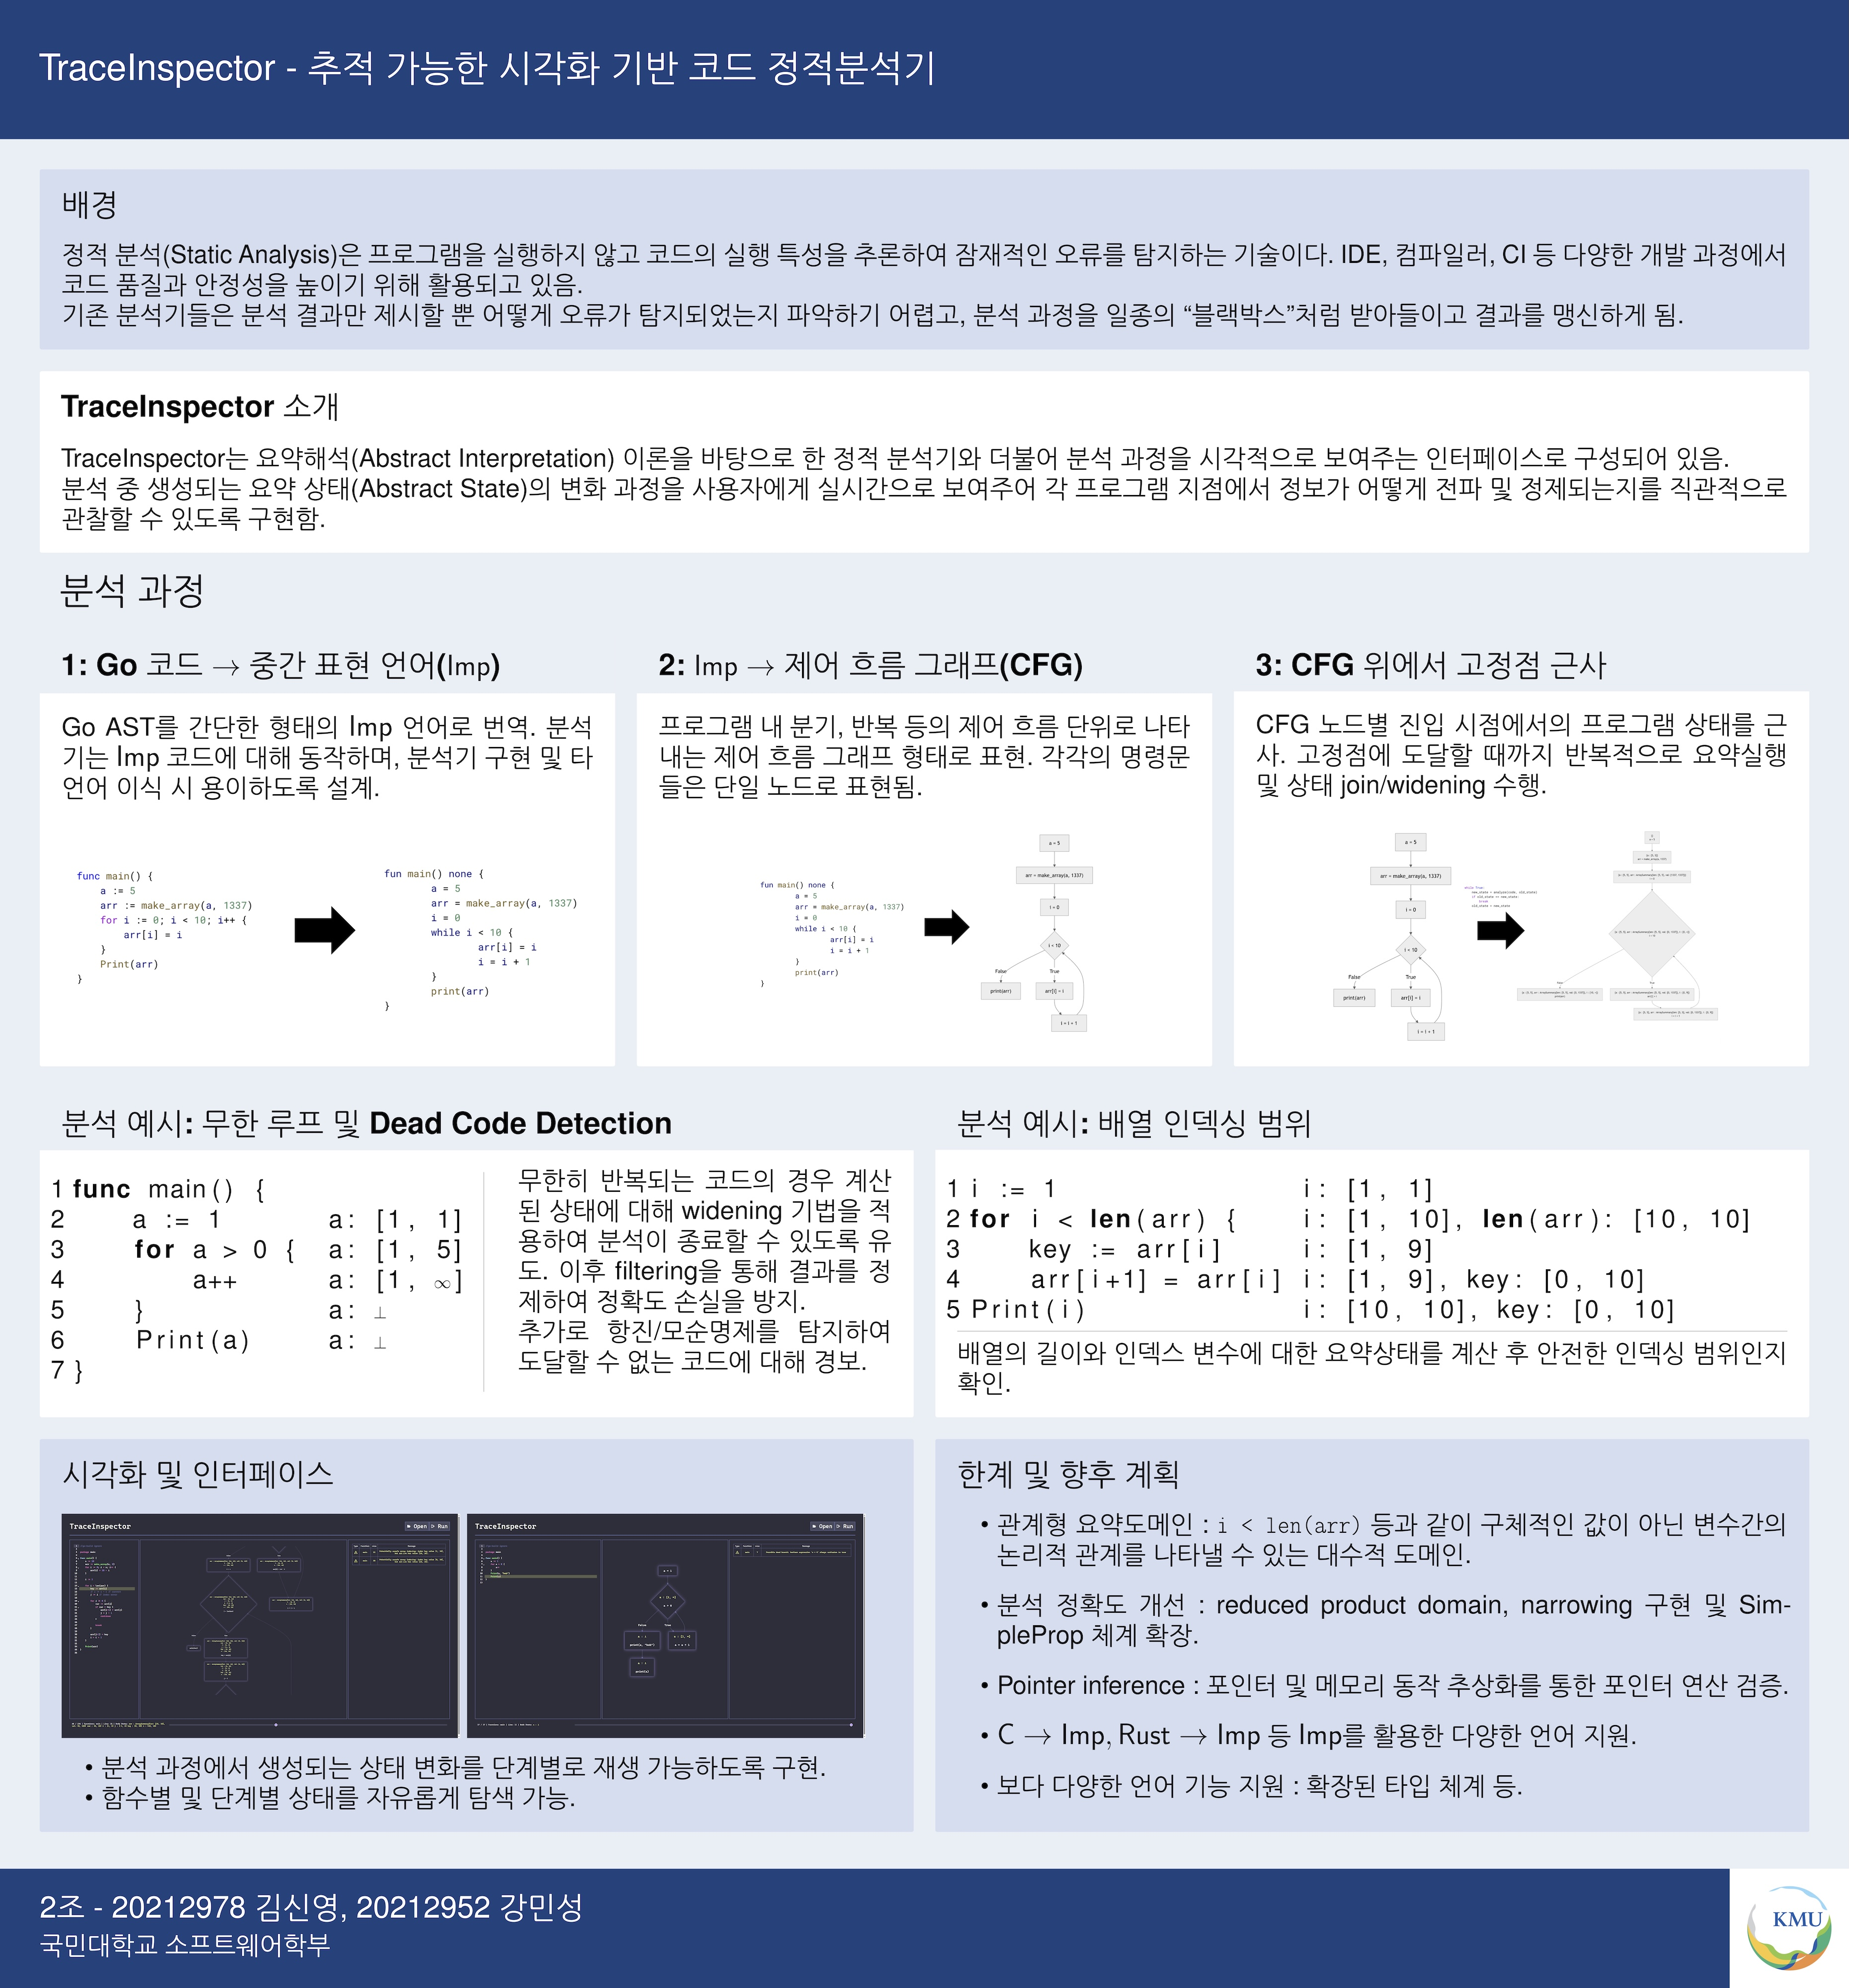
\includegraphics[width=\textwidth]{images/poster.jpg}
\end{center}




\begin{titlepage}
\thispagestyle{empty}

\centering

\vspace{8cm}

\Huge 결과보고서 발표자료

% \vspace{1cm}
% \rule{9cm}{3.5pt}
% \vspace{1cm}

% \begin{minipage}{0.5\textwidth}
%     \raggedright
%     \Large 3.1 결과보고서 \\
%     3.2 결과보고서 발표자료 \\
% \end{minipage} \par
% \vspace{1cm}
% \rule{9cm}{3.5pt}
\end{titlepage}
\slidepair{images/final_presentation/Slide1.png}{images/final_presentation/Slide2.png}
\slidepair{images/final_presentation/Slide3.png}{images/final_presentation/Slide4.png}
\slidepair{images/final_presentation/Slide5.png}{images/final_presentation/Slide6.png}
\slidepair{images/final_presentation/Slide7.png}{images/final_presentation/Slide8.png}
\slidepair{images/final_presentation/Slide9.png}{images/final_presentation/Slide10.png}
\slidepair{images/final_presentation/Slide11.png}{images/final_presentation/Slide12.png}
\slidepair{images/final_presentation/Slide13.png}{images/final_presentation/Slide14.png}
\slidepair{images/final_presentation/Slide15.png}{images/final_presentation/Slide16.png}
\slidepair{images/final_presentation/Slide17.png}{images/final_presentation/Slide18.png}
\slidepair{images/final_presentation/Slide19.png}{images/final_presentation/Slide20.png}
\slidepair{images/final_presentation/Slide21.png}{images/final_presentation/Slide22.png}
\slidepair{images/final_presentation/Slide23.png}{images/final_presentation/Slide24.png}
\slidepair{images/final_presentation/Slide25.png}{images/final_presentation/Slide26.png}
\slidepair{images/final_presentation/Slide27.png}{images/final_presentation/Slide28.png}
\clearpage


\begin{titlepage}
\thispagestyle{empty}

\centering

\vspace{1cm}

\Huge 제 4 장

\vspace{2.5cm}

{\fontsize{42pt}{42pt}
    멘토링 보고서
    \par
}

\end{titlepage}

\textbf{\large 1차 멘토링(2026-05-14, 강동호)} ~\\

TraceInspector 캡스톤 팀 단체 멘토링을 강동호 멘토와 진행하였다. 멘토님은 현업 개발자로, 풀스택 개발 및 실제 개발 환경에서의 경험이 많은 분이었다. 

우선적으로 우리가 개발한 소프트웨어 시연 및 설명을 진행하였다. 멘토님은 정적분석기가 무엇인지 알고 있었고 실제로 개발 단계에서도 활용하고 있었지만, 우리 소프트웨어만이 가진 장점과 기존에 있는 알고리즘 시각화 웹사이트나 디버거와의 차이점에 대해서도 물어보셨다. 이에 따라 어떤 알고리즘에 의해 분석이 일어나고, 어떤 방식으로 이러한 알고리즘 동작 방식을 보여주고자 했는지 설명을 드렸고 질의응답을 진행했다.

일차적으로 멘토님은 인터페이스상의 보완점들과 캡스톤프로젝트 관점에서 어떤 평가를 받을지에 대해서 말씀하셨다. 예시 코드 목록을 추가하여 사용자가 별도의 준비를 하지 않고도 우리 소프트웨어를 바로 사용해볼 수 있도록 수정하고, 캡스톤 프로젝트에서 큰 이목이나 좋은 평가를 받지 못하더라도 내용적으로 굉장히 깊이가 있고 단지 AI를 활용해서 포장한게 아니라 이 분야에 대해서 제대로 이해하고 구현한 인상을 받았다고 말씀하셨다. 

분석기에 대해서도 피드백을 주셨는데, 일차적으로 우리가 Go언어를 분석 대상으로 선정한 이유를 궁금해하면서 많은 사람들이 Go에 대해 크게 관심을 가지지 않을 것을 우려하셨다. 또한 우리 분석기가 여러 파일로 구성된 프로젝트를 분석 가능한지, 그리고 여러 프레임워크들이 통합된 복잡한 소스도 분석 가능하게끔 향후에 개선이 된다면 좋을 것 같다고 말씀하셨다. 멘토님 본인은 이게 실제 개발 환경에서 쓰인다기보단 정적 분석 알고리즘을 시각화하고 이해하는데 많은 도움이 될 것이라고 생각되고, 이런 주제가 참신하고 정적 분석에 대해 배워볼 수 있을 것 같다고 말씀하셨다.

마지막으로 멘토님께 프로젝트 외적으로 실제 개발 현장에서 정적 분석 도구 등 프로그래밍 언어론과 관련된 도구나 방법을 응용하고 있는지 물어보았고, 실제 개발자의 입장에서는 어떤 방식으로 소프트웨어를 분석하는 도구가 필요한지 여쭤보았다. 멘토님은 보안과 관련된 문제들이 굉장히 민감하다면서 이러한 취약점들을 분석해주는 분석기가 더 발전되면 유용할 것 같다고 말씀하셨고, LLM 역시 코드를 많이 생성하니 이러한 코드들도 신뢰할 수 있게 분석이나 검증이 가능하다면 좋을 것 같다고 말씀하셨다.

이번 멘토링을 통해 피드백은 물론, 스스로 어떻게 정적 분석이라는 개념을 남들에게 잘 설명할 수 있을까에 대해 고민을 하게 되었다. 이미 해당 분야를 들어보고 프로그래밍과 익숙한 멘토님께도 우리 정적분석기가 정확히 코드 시각화 서비스나 디버거랑 어떤 방면에 차이가 있는지 와닿을 수 있는 방식으로 설명하는게 어렵다는 것을 이번 기회를 통해 알게 되었다. 따라서 최종발표 준비를 할 때 이런 관점에서 설명을 준비하고 우리가 구현한 소프트웨어의 기능들과 한계들을 어떻게 잘 나타낼 수 있을지에 대해 다시금 생각해보게 되었다.

\clearpage

\textbf{\large 2차 멘토링(2026-05-17, 이광헌)} ~\\

TraceInspector 팀 멘토링을 이광헌 멘토와 진행하였다. 멘토링을 시작하기에 앞서, 멘토링 페이지에 게시된 멘토의 설명과 실제 멘토가 현재 진행중인 분야가 완전히 다름을 멘토가 언급했다. 하드웨어 설계보다는 AI모형 만드는 업무를 하고 있고, 이에 따라 멘토링 페이지에 본인 링크드인 등을 첨부하기를 희망한다는 얘기를 하였다.

이번 멘토링에서는 최종 발표자료가 준비되었던 관계로 멘토에게 우리 프로젝트 발표와 시연을 먼저 보여주었다. 멘토는 우리의 발표를 보고 다음과 같은 질문들을 하였다:
\begin{enumerate}
    \item 프로그램 실행 흔적 의미론을 설명하는 과정에서 테스팅은 유한한 갯수의 흔적만을 볼 수 있다고 나와있는데, 테스팅 coverage와 어떤 연관이 있는지?
    \item 이러한 요약해석 기법과 테스팅과 관계가 어떻게 되고 어떤 식으로 서로 활용할 수 있는지?
    \item Go나 C의 경우 정수 표현 범위가 정해져 있는데, 정적 분석기에서는 이러한 의미를 반영하는지?
\end{enumerate}

이처럼 우리 분석기 뿐만 아니라 정적 분석 자체에 대해 다양한 질문을 해주셨고, 특히 정적 분석기를 시각적으로 보여주는 인터페이스는 정말 참신한 아이디어이며 처음 본다는 말씀을 해주셨다. 

하지만 이전 멘토링과 마찬가지로, 실제로 가지고 있는 기술적 깊이와 구현된 분석기의 완성도와는 별개로 사용자와 평가자들이 보는 인터페이스 상에서 한눈에 분석 결과가 어떤 식으로 나오는지 보여주는 핵심적인 강조점이 잘 안보인다고 피드백을 하였다. 이에 실제로 오류가 검출되는 상태에서 문제가 되는 변수의 상태 등을 강조하여 시각적으로 돋보일 수 있다면 더 좋을거 같다고 조언하였고, 프로젝트의 방향 자체를 실제로 개발에서 많은 유저들이 사용하는 방향보다는 정적 분석이라는 분야에 대해 깊이 탐구하고 교육적 목표의 서비스를 구현했다는 점을 강조하는 방향이 더 유리할 것이라는 피드백을 주었다.

\clearpage


\begin{titlepage}
\thispagestyle{empty}

\centering

\vspace{1cm}

\Huge 제 5 장

\vspace{2.5cm}

{\fontsize{42pt}{42pt}
    회의록
    \par
}

\end{titlepage}

\textbf{\large 1차 주간 회의 (2026.03.06)}

첫 번째 팀 회의에서는 프로젝트 주제의 구체화와 역할 분담에 대해 논의하였다. 프로젝트의 목표를 Go 언어로 작성된 프로그램을 정적으로 분석하여 잠재적인 런타임 오류를 탐지하고 이를 사용자에게 제공하는 서비스로 정의하였다. 또한 사용자가 소스 코드를 업로드하고 분석 결과를 확인할 수 있도록 웹 기반 인터페이스를 구축하기로 결정하였으며, 인터페이스는 입력 및 업로드 영역과 분석 결과 시각화 영역으로 구성하기로 하였다.

역할 분담에 있어서는 분석기 이론 및 핵심 분석 로직 구현과 웹 인터페이스 개발을 분리하여 진행하기로 하였다. 이에 따라 김신영은 요약해석 기반 분석기의 의미론 설계 및 구현을 담당하고, 강민성은 프론트엔드 및 서비스 환경 구축을 담당하기로 결정하였다. 또한 다음 회의 전까지 Go 언어의 지원 범위를 정의하고 언어 요소별 요약 의미론의 초안을 설계하며, 동시에 웹 인터페이스의 기본 구조를 구현하기로 하였다.

~\\

\textbf{\large 2차 주간 회의 (2026.03.19)}

두 번째 팀 회의에서는 분석기와 프론트엔드 간의 인터페이스를 구체화하고, 제어 흐름 그래프(Control Flow Graph, CFG)의 출력 형식과 데이터 교환 방식을 확정하였다. 프론트엔드 구현 기술로 기존 JavaScript 기반 계획 대신 C\# Razor 프레임워크를 사용하기로 결정하였으며, 코드 입력 영역과 CFG 시각화 영역을 분리하는 사용자 인터페이스 구성을 논의하였다. 또한 분석기와 웹 서비스 간의 통신은 JSON 기반 인터페이스를 통해 수행하기로 결정하였다.

분석기 측에서는 Go 언어에 대한 요약해석 기반 정적 분석기의 설계를 위해 관련 문헌을 조사하고 언어 요소별 의미론 정의를 위한 기초 연구를 진행하였다. 구현 측면에서는 CFG 생성을 위한 Go 추상 구문 트리 순회 기능의 초안을 작성하였으며, 프로젝트 저장소를 개설하고 분석기와 프론트엔드 간의 입출력 명세를 확정하였다. 특히 CFG 출력, 분석 과정의 중간 상태 갱신 정보, 최종 오류 탐지 결과를 표준화된 형식으로 교환하기로 결정하여 향후 양 모듈의 독립적인 개발과 통합이 가능하도록 기반을 마련하였다.

~\\

\textbf{\large 3차 주간 회의 (2026.03.24)}

세 번째 팀 회의에서는 프론트엔드 인터페이스 초안에 대한 검토와 제어 흐름 그래프(Control Flow Graph, CFG) 생성 기능의 구현 현황을 점검하였다. 프론트엔드 측에서는 코드 입력 영역, 그래프 시각화 영역, 로그 출력 영역으로 구성된 초기 사용자 인터페이스 레이아웃을 제시하였으며, 향후 텍스트 에디터와 그래프 시각화 기능을 통합하기 위한 구체적인 구현 방향을 논의하였다. 또한 사용자 경험 측면에서 코드 작성, 분석 실행, 결과 확인이 하나의 화면에서 이루어질 수 있도록 인터페이스 구조를 정교화하기로 하였다.

분석기 측에서는 Go 프로그램으로부터 제어 흐름 그래프를 생성하는 기능의 구현을 완료하고, 간단한 예제 프로그램을 대상으로 정상적으로 동작함을 확인하였다. 아울러 요약해석 기반 정적 분석을 위한 이론적 설계를 지속적으로 진행하였으며, 분석 목표와 구현 난이도를 고려하여 적절한 요약 도메인을 검토하였다. 회의 결과 현재 분석기의 핵심 기반인 CFG 생성 단계는 완료된 것으로 판단하였으며, 향후에는 프로그램 상태를 표현하기 위한 요약 도메인과 의미론을 정립하고 분석 기능 구현에 집중하기로 결정하였다. 또한 Interval 도메인과 프로그램-레이블 쌍 집합 기반의 추상화 도메인을 우선적인 구현 대상으로 선정하였다.

~\\

\textbf{\large 4차 주간 회의 (2026.04.02)}

네 번째 팀 회의에서는 프론트엔드 및 분석기 구현 현황을 점검하고, 중간 발표 준비를 위한 향후 개발 계획을 수립하였다. 프론트엔드 측에서는 기존 HTML/CSS 기반 시제품을 TypeScript 및 React 기반 구조로 전환하는 작업을 완료하였으며, 코드 입력 기능을 위해 CodeMirror 에디터를 도입하고 그래프 시각화를 위해 Mermaid.js를 활용하기로 결정하였다. 이를 통해 향후 코드 편집, 분석 실행, 결과 시각화 기능을 통합한 웹 인터페이스를 구축할 수 있는 기반을 마련하였다.

분석기 측에서는 Go 언어의 추상적 의미론 설계를 지속적으로 수행하였으며, 반복문에 대한 widening 연산과 조건문 분기 처리 방안을 구체화하였다. 또한 구간(Interval) 추상 도메인을 구현하고, 추상 도메인을 모듈화된 인터페이스 형태로 설계하여 향후 다양한 추상 도메인을 손쉽게 추가할 수 있도록 구조를 개선하였다. 회의에서는 현재까지 CFG 생성 단계와 구간 도메인 구현이 완료되었음을 확인하였으며, 다음 단계로 추상 의미론의 실제 구현과 CFG 상에서의 기호 실행(symbolic execution)을 수행하기 위한 드라이버 코드를 개발하기로 결정하였다.

추가적으로 중간 발표 준비를 위해 현재까지의 구현 성과를 정리하고, 분석기와 프론트엔드의 핵심 기능을 시연할 수 있는 데모 환경을 구축하는 방안을 논의하였다. 향후에는 추상 의미론 구현을 완료하고, 웹 인터페이스에 텍스트 에디터 및 그래프 시각화 기능을 통합하는 작업을 중점적으로 진행하기로 하였다.

~\\

\textbf{\large 5차 주간 회의 (2026.04.06)}

다섯 번째 팀 회의에서는 중간 발표 준비와 함께 프론트엔드 및 분석기 구현 현황을 점검하였다. 프론트엔드 측에서는 CodeMirror 기반 코드 편집기를 인터페이스에 통합하였으며, 제어 흐름 그래프(CFG) 정보를 해석하고 시각화하기 위한 기능 구현에 착수하였다. 또한 현재까지의 개발 결과와 향후 인터페이스 확장 계획을 정리하여 중간 발표 자료 제작을 진행하였다.

분석기 측에서는 Imp 언어의 의미론 정의와 Go 프로그램을 Imp 중간 표현으로 변환하는 번역기를 구현하였으며, Imp 프로그램에 대한 CFG 생성 알고리즘을 완성하였다. 이를 통해 코드 전처리 단계가 완료되었으며, 이후에는 설계한 요약 의미론을 기반으로 실제 요약해석 프레임워크와 분석 알고리즘 구현에 집중하기로 하였다. 또한 중간 발표에서는 분석기와 프론트엔드 영역을 분리하여 각각 이론적 배경, 구현 현황, 인터페이스 설계 및 향후 개발 계획을 소개하기로 결정하였다.

~\\

\textbf{\large 6차 주간 회의 (2026.04.16)}

여섯 번째 팀 회의에서는 중간 발표 자료를 최종 검토하고 시연 영상을 촬영하는 한편, 분석기와 프론트엔드 간의 인터페이스를 보완하기 위한 논의를 진행하였다. 프론트엔드 측에서는 Go 언어 구문 강조 기능을 코드 에디터에 적용하였으며, Go 소스 파일을 직접 불러와 편집기에 표시하는 기능을 구현하였다. 또한 그래프 시각화와 백엔드 서버 구축을 위해 Express 기반 환경을 도입하여 통합 작업을 진행하였다.

분석기 측에서는 함수 단위 분석을 지원하기 위해 CFG 노드 식별 체계를 개선하고, 함수 이름과 연계된 고유 식별자를 생성하도록 구조를 수정하였다. 이에 따라 JSON 출력 형식도 함께 갱신되었으며, 고정점 계산 프레임워크와 요약 도메인 구현을 본격적으로 도입하기 시작하였다. 회의에서는 중간 발표 자료와 시연 영상을 최종 점검하였고, 함수별 CFG 출력과 분석 중간 결과의 교환 형식을 확정하여 프론트엔드와 분석기 간의 연동 기반을 강화하였다.

~\\

\textbf{\large 7차 주간 회의 (2026.04.30)}

일곱 번째 팀 회의에서는 분석기 출력 결과를 검토하고 프론트엔드의 그래프 시각화 결과에 대한 피드백을 진행하였다. 프론트엔드 측에서는 그래프 렌더링 기능과 탭 인터페이스를 개선하였으며, 시연 환경의 안정성을 확보하기 위해 별도의 웹 서버를 구축하였다. 또한 분석기에서 제공하는 디버그 출력 기능을 활용하기 위한 결과 출력 영역 구현을 시작하였다.

분석기 측에서는 반복문을 포함한 언어의 주요 구성 요소를 처리할 수 있는 첫 번째 분석기 버전을 완성하였으며, 삽입 정렬과 같은 예제 프로그램을 대상으로 분석 결과를 검증하였다. 특히 고정된 크기의 배열에 대한 참조 범위 오류를 성공적으로 탐지함으로써 분석기의 기본 기능이 정상적으로 동작함을 확인하였다. 또한 분석 과정 중 발생하는 상태 변화 정보를 프론트엔드와 공유하기 위한 출력 형식을 정의하고, 이에 맞추어 상태 갱신 이벤트를 생성하도록 구현하였다. 회의에서는 정보, 경고, 오류 메시지 및 상태 갱신을 위한 JSON 통신 규격을 확정하고 향후 사용자 인터페이스 개선 방향을 함께 논의하였다.

~\\

\textbf{\large 8차 주간 회의 (2026.05.07)}

여덟 번째 팀 회의에서는 분석기와 프론트엔드 간 상태 출력 형식을 표준화하고, 양 시스템의 연동 상태를 점검하였다. 프론트엔드 측에서는 상태 출력 창을 구현하는 과정에서 사용자 인터페이스를 전반적으로 개선하였으며, 창 여백 제거, 스크롤 동작 개선, Upload 및 Run 기능 통합, 탭 관련 버그 수정 등 다수의 사용성 개선 작업을 수행하였다.

분석기 측에서는 디버그 출력 기능과 도메인 연산 결과를 선택적으로 활성화할 수 있도록 수정하여, 실제 실행 시에는 JSON 기반 결과만 출력하도록 구조를 개선하였다. 또한 프론트엔드와의 교차 검증을 통해 출력 형식을 지속적으로 조정하고 호환성을 검증하였다. 회의 결과 상태 출력 창, 하이라이트 기능, 상태 변화 탐색을 위한 슬라이더 기능을 포함한 최종 인터페이스 구현 방향을 확정하였으며, 포스터 초안 및 최종보고서 작성을 위한 준비 작업을 병행하기로 하였다.

~\\

\textbf{\large 9차 주간 회의 (2026.05.14)}

아홉 번째 팀 회의에서는 분석기의 요약 도메인 관련 오류 수정과 프론트엔드 인터페이스 개선 작업을 점검하고, 프로젝트 결과물 정리를 위한 포스터 및 발표 자료 작성 계획을 논의하였다. 프론트엔드 측에서는 사용자 인터페이스를 전반적으로 개편하여 색상 테마를 Nord에서 Dracula로 변경하였으며, 상태 변화가 보다 명확하게 드러나도록 그래프 출력 형식을 개선하였다. 또한 분석 과정의 변화를 시간 순서대로 확인할 수 있도록 타임라인 슬라이더를 추가하고, 다양한 시각적 효과와 하이라이트 기능을 보강하였다.

분석기 측에서는 구간 추상 도메인과 확장 정수(extended integer) 연산에서 발견된 건전성 문제를 수정하였으며, 고정점 계산 이후의 상태를 활용하는 post-fixpoint analysis를 구현하였다. 이를 통해 반복문 및 조건문 가드가 항상 참 또는 거짓으로 평가되는 경우를 탐지하여 경고를 생성하는 기능을 추가하였다. 회의에서는 포스터 작성을 완료하여 제출하였고, 최종 발표 자료와 요약 결과 보고서 작성을 위한 마무리 작업 계획을 수립하였다.

\clearpage


\begin{titlepage}
\thispagestyle{empty}

\centering

\vspace{1cm}

\Huge 주 의 문

\vspace{2.5cm}

% {\fontsize{42pt}{42pt}
%     결과보고서
%     \par
% }

\begin{minipage}{0.8\textwidth}
    \large 2026년 다학제간캡스톤디자인I 최종보고서 \\
    \textbf{TraceInspector} \\
    \vspace{0.2cm}
    \rule{\linewidth}{0.8pt} \par
    \vspace{0.2cm}
    \raggedright
    발행인 : \textbf{김신영, 강민성} \\
    발행일 : 2026년 6월 19일 \\
    발행처 : 국민대학교 소프트웨어융합대학 소프트웨어학부 \\
    주소 : (136-702) 서울시 성북구 정릉동 861-1 \\
    \vspace{0.2cm}
    \rule{\linewidth}{0.8pt} \par
    \vspace{0.2cm}
    \begin{enumerate}
        \item 이 보고서는 국민대학교 소프트웨어융합대학 소프트웨어학부에서 개설한 교과목 다학제간캡스톤디자인I 에서 수행한 프로젝트 최종보고서 입니다.
        \item 이 보고서의 내용은 국민대학교 소프트웨어학부 및 위 발행인들의 서면 허락없이 사용되거나, 재가공 될 수 없습니다.
    \end{enumerate}
    \rule{\linewidth}{0.8pt} \par
\end{minipage} \par
\vspace{1cm}
\end{titlepage}

\end{document}